% Options for packages loaded elsewhere
\PassOptionsToPackage{unicode}{hyperref}
\PassOptionsToPackage{hyphens}{url}
%
\documentclass[
  12pt,
]{book}
\usepackage{lmodern}
\usepackage{amssymb,amsmath}
\usepackage{ifxetex,ifluatex}
\ifnum 0\ifxetex 1\fi\ifluatex 1\fi=0 % if pdftex
  \usepackage[T1]{fontenc}
  \usepackage[utf8]{inputenc}
  \usepackage{textcomp} % provide euro and other symbols
\else % if luatex or xetex
  \usepackage{unicode-math}
  \defaultfontfeatures{Scale=MatchLowercase}
  \defaultfontfeatures[\rmfamily]{Ligatures=TeX,Scale=1}
\fi
% Use upquote if available, for straight quotes in verbatim environments
\IfFileExists{upquote.sty}{\usepackage{upquote}}{}
\IfFileExists{microtype.sty}{% use microtype if available
  \usepackage[]{microtype}
  \UseMicrotypeSet[protrusion]{basicmath} % disable protrusion for tt fonts
}{}
\makeatletter
\@ifundefined{KOMAClassName}{% if non-KOMA class
  \IfFileExists{parskip.sty}{%
    \usepackage{parskip}
  }{% else
    \setlength{\parindent}{0pt}
    \setlength{\parskip}{6pt plus 2pt minus 1pt}}
}{% if KOMA class
  \KOMAoptions{parskip=half}}
\makeatother
\usepackage{xcolor}
\IfFileExists{xurl.sty}{\usepackage{xurl}}{} % add URL line breaks if available
\IfFileExists{bookmark.sty}{\usepackage{bookmark}}{\usepackage{hyperref}}
\hypersetup{
  pdftitle={PhD},
  pdfauthor={Maria Rivera Araya},
  hidelinks,
  pdfcreator={LaTeX via pandoc}}
\urlstyle{same} % disable monospaced font for URLs
\usepackage{longtable,booktabs}
% Correct order of tables after \paragraph or \subparagraph
\usepackage{etoolbox}
\makeatletter
\patchcmd\longtable{\par}{\if@noskipsec\mbox{}\fi\par}{}{}
\makeatother
% Allow footnotes in longtable head/foot
\IfFileExists{footnotehyper.sty}{\usepackage{footnotehyper}}{\usepackage{footnote}}
\makesavenoteenv{longtable}
\usepackage{graphicx}
\makeatletter
\def\maxwidth{\ifdim\Gin@nat@width>\linewidth\linewidth\else\Gin@nat@width\fi}
\def\maxheight{\ifdim\Gin@nat@height>\textheight\textheight\else\Gin@nat@height\fi}
\makeatother
% Scale images if necessary, so that they will not overflow the page
% margins by default, and it is still possible to overwrite the defaults
% using explicit options in \includegraphics[width, height, ...]{}
\setkeys{Gin}{width=\maxwidth,height=\maxheight,keepaspectratio}
% Set default figure placement to htbp
\makeatletter
\def\fps@figure{htbp}
\makeatother
\setlength{\emergencystretch}{3em} % prevent overfull lines
\providecommand{\tightlist}{%
  \setlength{\itemsep}{0pt}\setlength{\parskip}{0pt}}
\setcounter{secnumdepth}{5}
\usepackage{booktabs}
\usepackage{booktabs}
\usepackage{longtable}
\usepackage{array}
\usepackage{multirow}
\usepackage{wrapfig}
\usepackage{float}
\usepackage{colortbl}
\usepackage{pdflscape}
\usepackage{tabu}
\usepackage{threeparttable}
\usepackage{threeparttablex}
\usepackage[normalem]{ulem}
\usepackage{makecell}
\usepackage{xcolor}
\usepackage[]{natbib}
\bibliographystyle{plainnat}

\title{PhD}
\author{Maria Rivera Araya}
\date{2021-10-03}

\begin{document}
\maketitle

{
\setcounter{tocdepth}{1}
\tableofcontents
}
\hypertarget{thesis}{%
\chapter{Thesis}\label{thesis}}

\hypertarget{acknowledgements}{%
\chapter*{Acknowledgements}\label{acknowledgements}}
\addcontentsline{toc}{chapter}{Acknowledgements}

I sincerely thank:

\begin{itemize}
\item
  My supervisors Michael Bird, Sean Ulm, Cassandra Rowe, Vladimir Levchenko and Jonathan Tyler for supporting my ideas throughout my PhD candidature. Thanks to Michael Bird for financial support during my fieldwork and labwork throughout my PhD.
\item
  Vladimir Levchenko and Patricia Gadd for supporting my AINSE PGRA application, for hosting me at ANSTO several times through the course of my PhD.
\item
  John Tibby, Ulrike Proske and Kathryn Taffs for their help interpreting diatom assemblages. Anne Alexandre for her help identifying phytoliths.
\item
  The Traditional Owners of the lands and waters we carried out fieldwork, including Anggamudi (also known as Angkamuthi), Wuthahti (alternatively Wuthathi) and Yadhaigana (alternatively Yadhaykenu). In particular Charles Woosop and the Apudthama Land Trust.
\item
  The AINSE team (Michael Rose, Sandy O' Connor, Michelle Durant, Nerissa Phillips) for their help during my AINSE PGRA visits
\item
  My partner Maru, my family in Costa Rica
\item
  My lab colleagues and friends
\item
  I am also very grateful for the financial support provided for this PhD research project by the following organisations:
\item
  Australian Research Council (Laureate Fellowship to Michael Bird)
  Grant \# FL140100044
\item
  Australian Institute of Nuclear Science and Engineering (AINSE)
  PGRA- Post Graduate Research Award \# 12357
\item
  Centre of Excellence for Australian Biodiversity and Heritage
  Grant \# CE170100015
\item
  Universidad de Costa Rica through the Academic Mobility Program
\end{itemize}

\hypertarget{statement-of-the-contributions-of-others}{%
\chapter*{Statement of the Contributions of Others}\label{statement-of-the-contributions-of-others}}
\addcontentsline{toc}{chapter}{Statement of the Contributions of Others}

Standard contributions were made by the supervisory team of Professor Michael Bird, Professor Sean Ulm, Dr.~Cassandra Rowe, Dr.~Jonathan Tyler and Dr.~Vladimir Levchenko. This assistance included project design, technical support, and revisions and editing of this thesis.

\begin{table}

\caption{\label{tab:st3}Contributions of others to the thesis}
\centering
\begin{tabular}[t]{cc>{\centering\arraybackslash}p{5cm}}
\toprule
Nature of assistance & Contribution & Names of contributors\\
\midrule
 & Proposal writing & Prof. Michael Bird\\
\cmidrule{2-3}
 & Data Analysis & Prof. Michael Bird, Dr. Cassandra Rowe, Vladimir Levchenko\\
\cmidrule{2-3}
\multirow{-3}{*}{\centering\arraybackslash Intellectual support} & Editorial  assistance & Prof. Michael Bird, Prof.  Sean Ulm, Dr. Cassandra Rowe\\
\cmidrule{1-3}
 & Research costs & Prof. Michael Bird\\
\cmidrule{2-3}
 & Stipend & JCU Postgraduate Research Scholarship\\
\cmidrule{2-3}
\multirow{-3}{*}{\centering\arraybackslash Financial support} & Travel and research training & Centre of Excellence for Australian Biodiversity and Heritage\\
\cmidrule{1-3}
 & Research assistance & Prof. Michael Bird, Dr. Cassandra Rowe, Vladimir Levchenko\\
\cmidrule{2-3}
\multirow{-2}{*}{\centering\arraybackslash Data collection} & Sample collection & Prof. Michael Bird, Dr. Cassandra Rowe, Rainy Comley, Costjin Zwart\\
\bottomrule
\end{tabular}
\end{table}



\hypertarget{abstract}{%
\chapter*{Abstract}\label{abstract}}
\addcontentsline{toc}{chapter}{Abstract}

There are no long-term records of climatic and environmental change from Cape York Peninsula in the tropical savannas of northeast Australia. This scarcity has constrained the development and understanding of climate and environmental change in the Australian's tropics, and thereby the ability to provide context for the long period of human occupation of the region. Lake sediment archives are widely used to recognize changes in climate, precipitation and anthropogenic activities with the potential to significantly extend the length of available observational record by many millennia. Despite the common use of lake sediment proxy indicators to reconstruct climate and environmental histories, existing research demonstrates the complications associated with building robust and accurate chronologies, and interpreting the meaning of observed changes observed from multiple physical, biological and chemical sources of information.

This study was based upon a 1.72 m sediment core from Sanamere Lagoon (11.123°S 142.359°E) with the aim to develop a new record of climate and environmental change for northern Cape York Peninsula. The record spans the last \textasciitilde33 thousand calibrated years before the present (ka), based on a robust chronology established by comparing age-models derived from multiple carbon fractions (pyrogenic carbon derived from hydrogen pyrolysis -hypy fraction-, macrocharcoal, microcharcoal, pollen concentrate, bulk sediment and cellulose). The age-depth model derived from the hypy fraction was the most reliable and consistent with the stratigraphic changes identified along the core, removing allochthonous carbon and postdepositional contamination. This chronology provided the base for the climatic and environmental reconstructions from the Sanamere sediment core presented in this thesis.

Time series based on diatoms, phytoliths, hypy fractions, stable isotopes and elemental geochemistry (ITRAX micro X-ray fluorescence scanning) were used to understand the evolution of environmental conditions in the area surrounding Sanamere Lagoon. Four main periods of environmental change were identified (33 - 29.1 ka, 29.1 - 18.2 ka, 18.2 - 9.7 ka and 9.7 ka - present). During the first period, the lagoon formed by collapse of underlying laterite karst terrain, to a level below the local water table, ensuing a continuous record. The lagoon was filled following a wet event, likely related to a southward shift of the Intertropical Convergence Zone (ITCZ) during low sea levels. The results suggest a dominance of dry conditions during the first two identified periods 33 - 18.2 ka. However, no evidence of extreme dry conditions during the Last Glacial Maximum are recorded in the lake sediments. During this time Sanamere Lagoon was a small and shallow water body, with limited organic input. The lagoon expanded and deepened during 18.2 - 9.7 ka, in particular starting at 12.4 ka, following wetter conditions derived from increased monsoon activity and approach of the ocean following sea level rise. The last time period (after 9.7 ka) records increased organic input, related to wet conditions. Between 4.9 - 4.2 ka, high sedimentation rates and changes in the diatom assemblage and geochemical indicators indicate further deepening of the lagoon. Finally, after a slight decrease in rainfall from \textasciitilde{} 4.2 ka, the lagoon stabilised to reach modern conditions.

Changes in vegetation and fire were recorded using phytoliths and the hypy fractions. The sequence was characterized by the presence of sedges and woody taxa from the beginning to \textasciitilde{} 9.7 ka, with a minimal contribution from grasses. The redevelopment of the monsoon, between 18.2 and 9.7 ka, sustained the dominance of members of Cyperaceae at the site. After 9.7 ka, and particularly after 7.2 ka, wetter conditions sustained a higher proportion of arboreal taxa during the early and middle Holocene, compared to earlier periods. While fire activity is recorded through the entire sequence, activity is increased only during the Holocene. Peaks in the accumulation rates of the hypy fraction at 9.3 and 7.4 - 7.1 ka indicate an increment in fire activity (sustained by a higher availability of biomass to burn) also during the early and middle Holocene.

The results suggest that sea level was a defining feature of the climate and development of Sanamere Lagoon since its formation. The position of the ITCZ and monsoon activity were also determinant factors in the development of the lagoon. This thesis also brings new insights into the changes in environmental conditions in northern Australia, a region with great potential to understand the interactions between climate, vegetation, fire and humans using a long-term perspective.

This thesis makes a significant contribution to the understanding of environmental change (vegetation, fire and hydrology) in Australia's monsoonal tropics over the last 33,000 years. It also provides a method for building reliable radiocarbon chronologies in lake sediments, as reliable chronologies are critical for the interpretation of palaeoenvironmental archives in the tropics. Further records of environmental change from tropical Australia, a region that has been continuously inhabited by indigenous Australians for 65,000 years, will enable a more detailed understanding of regional monsoon (palaeo)dynamics and human environment interactions.

\hypertarget{introduction-and-aims}{%
\chapter{Introduction and aims}\label{introduction-and-aims}}

\hypertarget{introduction}{%
\section{Introduction}\label{introduction}}

The tropics are home to approximately half of the world's population and occupy one third of its landmass. Alarmingly, a growing body of evidence shows that these areas will feel the heaviest effects of global warming and climate change \citep{wheelerClimateChangeImpacts2013, frankEffectsClimateExtremes2015, diffenbaughQuantifyingInfluenceGlobal2017}. Increasing the number of local climatic and vegetation change records from the tropics is required to inform climatic projections and modelling relevant to managing these future changes. These models can contribute to tackling the environmental and economic impact of climate extremes (such as floods, droughts and related changes in fire activity) in our societies. By lengthening the environmental and climatic data record to thousands of years beyond the historical instrumental record, the uncertainty in projections of future environmental change can be reduced.

In particular, knowledge generated by studying long-term palaeoenvironmental records from northern Australia provides important contextual information about climate variability in the Australian sub-tropics, humid and monsoonal tropics. This information can be used, for instance, to improve environmental management strategies for Australian tropical savannas in the future, given their socio-economic importance for agriculture and pastoralism \citep{stoecklKeyIndustriesAustralia2007}.

Northern Australia is one of the world's most crucial places to pursue long-term studies regarding human-environment relationships, given that there is evidence of at least 65,000 years of human occupation \citep{clarksonHumanOccupationNorthern2017}. Investigating this area of the world contributes to the understanding of the connections between environmental conditions and human societies.

To understand climate variability and sensitivity, knowledge of long-term changes on millennial timescales is necessary. Records derived from lake sediments have proven to be useful across a range of geographical areas in recognizing changes in climate, precipitation and anthropogenic activities \citep{lengPalaeoclimateInterpretationStable2004, meyersLacustrineSedimentaryOrganic1999}. Lake sediments contain geochemical proxies from a range of sources including the lake body and lake catchment and thus can record environmental and hydrological changes controlled by climate variations and anthropogenic activities. Records derived from lake sediments have proven to be useful across a range of geographical areas in recognizing changes in land use, palaeoclimate, palaeoecology and palaeohydrology. Indeed, palaeolimnology, the use of lakes to derive information about the past environmental conditions, is now a well-established field of study that makes essential contributions to our understanding of past environmental conditions \citep{cohenPaleolimnologyHistoryEvolution2003, catalanGlobalChangeRevealed2013}.

This project focuses on understanding the environmental history and geochronology of the Sanamere Lagoon in northern Cape York, tropical northern Australia (Figure \ref{fig:fig-CP}). Two main considerations guided the development of the project: 1) Geochronology: to provide the information upon which to base optimized dating protocols for tropical lake sediments and 2) Environmental change and palaeohydrology: to create a high-resolution record of environmental change (sedimentological, vegetation and fire) for a region located in the tropical savannas of northern Australia.

\begin{figure}

{\centering 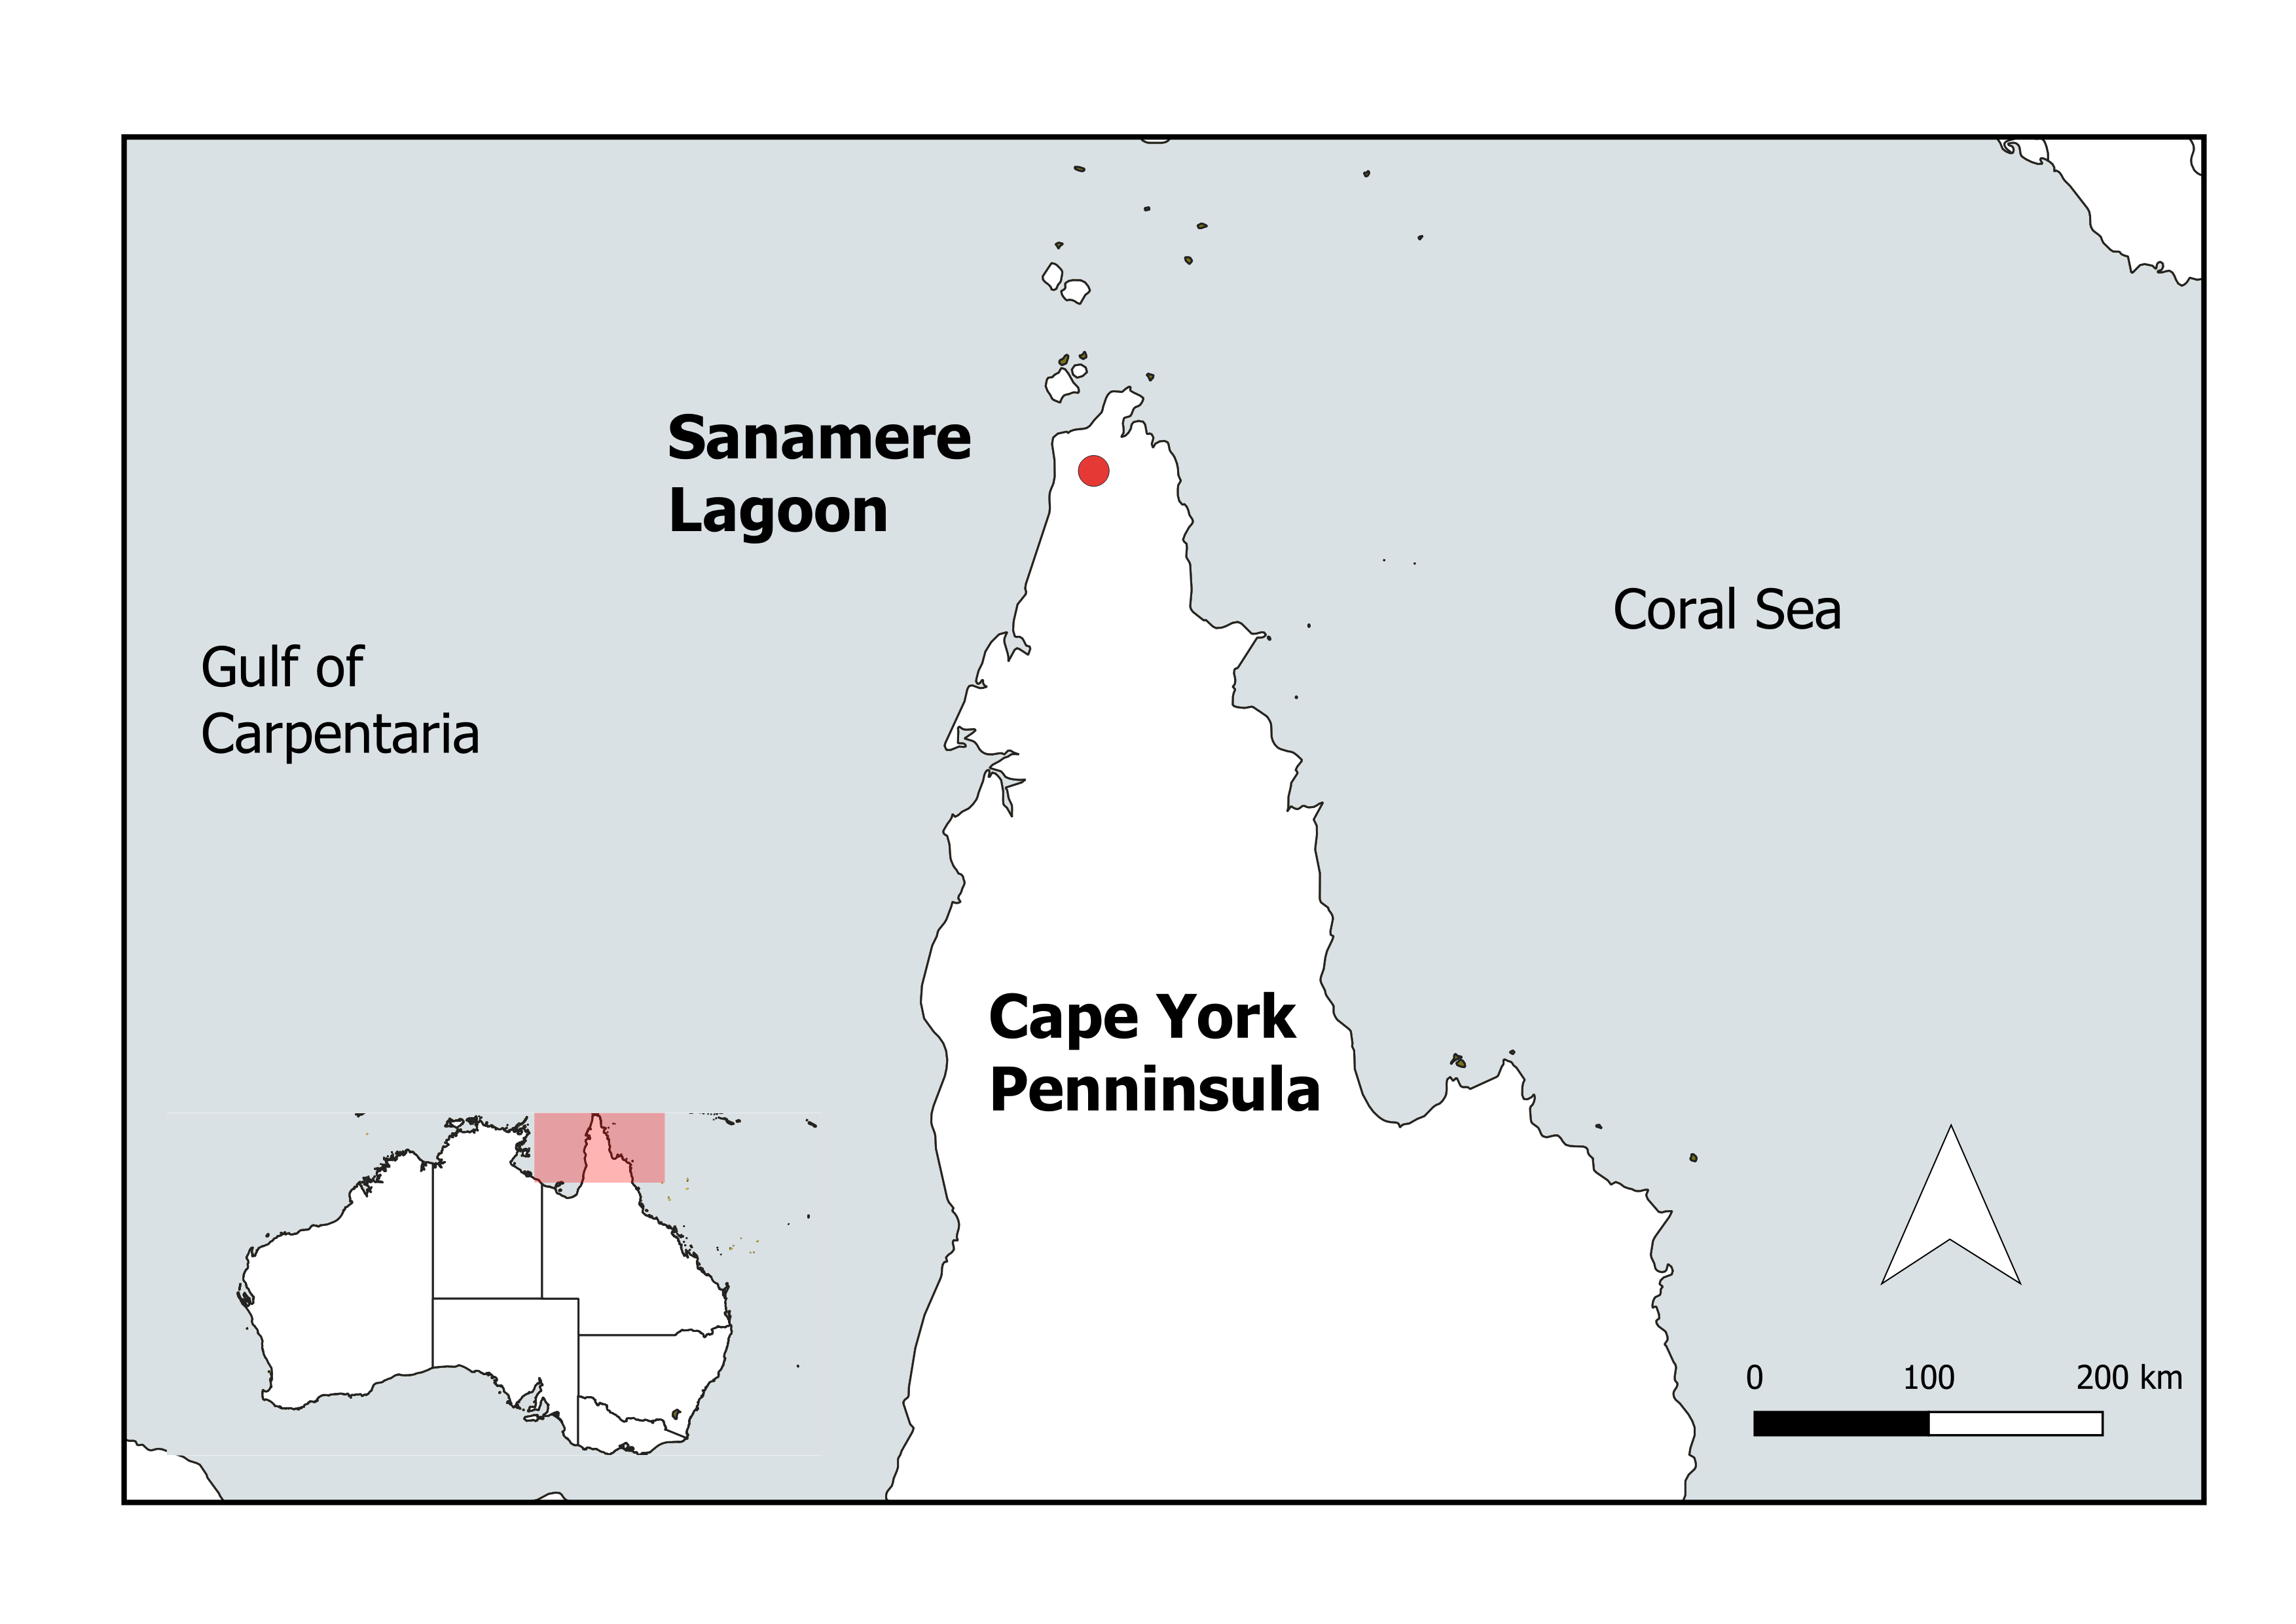
\includegraphics[width=0.8\linewidth]{C:/Users/Maria Jose Rivera/Documents/PhD/Figs/SAN_map_25_04_20} 

}

\caption{Sanamere Lagoon in Cape York Peninsula}\label{fig:fig-CP}
\end{figure}



\hypertarget{thesis-aims}{%
\section{Thesis aims}\label{thesis-aims}}

\hypertarget{geochronology}{%
\subsection{Geochronology}\label{geochronology}}

\begin{itemize}
\tightlist
\item
  Aim I. Develop a protocol for building robust chronologies in tropical lake sediments using radiocarbon dating
\end{itemize}

Precise and accurate radiocarbon ages up the radiocarbon dating limit of \textasciitilde{} 50,000 years ago (and the chronologies derived from dating) are critical for testing hypotheses of synchronous (or asynchronous) archaeological, environmental and climatic change and the interpretation of proxy records derived from lake sediment sequences. Although there have been many studies investigating methods for improving chronologies from lake sedimentary archives, most research attempting to identify the material most appropriate for dating has focused on temperate and arctic regions. A single exception deals with peat cores in the tropics, where pollen was found to be the most reliable dating fraction \citep{wustComparisonRadiocarbonAges2008}. The application of hydrogen pyrolysis (hypy) pretreatment to isolate stable polycyclic aromatic carbon (``Hypy fraction'') for dating appears to offer a viable approach to constructing chronologies from tropical organic spring deposits \citep{fieldUntanglingGeochronologicalComplexity2018}, where other materials have been demonstrated to be unreliable. In addition, no previous studies carried out in tropical lakes have tested a diversity of carbon fractions in the same sediment core, as the present study is proposing, to optimize a dating protocol to produce robust lacustrine chronologies.

Furthermore, previous studies have reported significant discrepancies between dates for different carbon fractions in lake sediments from the same depth. For example, in boreal and arctic regions, lake sediment, wood and charcoal were found to be older than other macrofossil types, usually by several hundred years \citep{oswaldEffectsSampleMass2005}. Discrepancies have been found also within different types of macrofossils, with some of them more prone to an apparent `reservoir effect'. This effect can result in anomalously old radiocarbon ages of the dated samples by introducing preaged carbon \citep{alvesWorldwideMarineRadiocarbon2018}. For example, wood and charcoal were found to be older than other plant remains in some ecosystems. A possible explanation is the slower decomposition and longer terrestrial residence time of these materials \citep{oswaldEffectsSampleMass2005}

Additionally, several studies have demonstrated that there are significant uncertainties associated with dating bulk sediment \citep{bjorckHighresolution14CDated1998, wustComparisonRadiocarbonAges2008}. Although organic-rich sediments from lake deposits provide diverse materials to analyze for radiocarbon dating, there is considerable uncertainty regarding which organic fraction yields the most reliable radiocarbon ages and how these `ages' relate to the actual time of deposition of the material. In addition, the relatively hot and moist conditions that characterize much of the tropics influence the preservation of materials that could be analyzed in these settings. For instance, aberrant radiocarbon results could be linked with poorly preserved or degraded charcoal, for example when the combustion yields are lower than usually expected (50-60 \% C by weight) \citep{highamRadiocarbonDatingCharcoal2009}. Also, the materials used for radiocarbon dating are prone to contamination and reservoir effects, which are known to cause serious deviations in the obtained ages, relative to age of deposition. Therefore, as well as providing a robust chronology against which to interpret the record of environmental change at Sanamere Lagoon, the creation of more effective and efficient pretreatment procedures for radiocarbon analyses is relevant to improving laboratory efficiencies, in turn lowering costs and increasing throughput.

The Sanamere Lagoon sequence offers a `best case', `tropical' opportunity to a) investigate the consistency of the age models derived from the different carbon fractions that were radiocarbon dated, b) study the causes of potential inconsistences in the radiocarbon dates and correlate the dates with potential disturbances/events along the length of the core.

Research questions:

\begin{itemize}
\item
  How do the radiocarbon dates derived from diverse carbon fractions relate to each other within individual samples, and over time in multiple samples along the core?
\item
  How and why do reservoir and contamination effects manifest themselves in the radiocarbon measurements of different organic fractions?
\item
  How consistent are differences observed between the dated carbon fractions?
\item
  How might differences between the `true' and `observed ages' be minimized by selection and dating of a particular `ideal' fraction?
\end{itemize}

\hypertarget{environmental-change-and-palaeohydrology}{%
\subsection{Environmental change and palaeohydrology}\label{environmental-change-and-palaeohydrology}}

\begin{itemize}
\item
  Aim II. Reconstruct past climatic variability in northern Cape York Peninsula using the Sanamere Lagoon sediment sequence
\item
  Aim III. Reconstruct past vegetation and fire activity in northern Cape York Peninsula using the Sanamere Lagoon sediment sequence
\end{itemize}

Although Australia has been the target of large projects (OZ-INTIMATE, Australian INTIMATE) aiming to develop a climate event stratigraphy for the region \citep{reevesPalaeoenvironmentalChangeTropical2013}, there are very few records of past terrestrial environmental change of any time depth for the Australian tropics outside the Atherton Tablelands in the wet tropics (refer to chapter 2 for more details about past environmental records). Most (inland) pollen and charcoal records have focused on wetter parts of the region that contain extensive, permanent lakes and swamps or are from the marine realm, in association with marine environmental proxies. Continuous records of environmental change are scarce in the tropical savannas beyond the Holocene, given the poor preservation of proxy material due to the ephemeral nature of most lakes as a result of seasonality in rainfall. A few studies in the Pilbara region of northwestern Australia, the Northern Territory and northern Cape York have yielded some insights into the hydroclimate of the region. Most research has focused in building Holocene pollen records in Groote Eylandt in the Gulf of Carpentaria \citep{shulmeisterHolocenePollenRecord1992, shulmeisterMorphologyChronostratigraphyCoastal1992, shulmeisterAustralasianEvidenceMidholocene1999}, Vanderlin Island \citep{prebbleHolocenePollenDiatom2005}, Mornington Island \citep{mossEnvironmentalContextLate2015}, Bentinck Island \citep{mackenzieGeochemicalInvestigationSouth2017}, and northern Cape York \citep{rowePalynologicalInvestigationHolocene2007, roweLateHoloceneSwamp2015}. However, the only studies focusing in palaeohydrology in tropical Australia have been pursued in Lake Carpentaria \citep{jonesLateQuaternaryEvolution1988, mccullochStrontiumIsotopeVariations1989a, reevesPalaeoenvironmentalChangeGulf2007, reevesSedimentaryRecordPalaeoenvironments2008, torgersenLateQuaternaryHydrological1985a, devriendtLateQuaternaryEnvironment2011}. Other studies have reconstructed the terrestrial palaeoclimate records, which have been interpreted as providing indirect evidence of palaeohydrological conditions. More recently, palaeoecological records have also emerged from the Kimberley region in Western Australia \citep{fieldLateQuaternaryRecord2017, dennistonStalagmiteRecordHolocene2013} (see section \ref{pastclimate}).

During the last 33 ka, important environmental changes have influenced northern Australia (e.g.~end of the last glacial period, reactivation of the monsoon, sea level changes, and the onset/intensification of El Niño-Southern Oscillation). These changes impacted and altered the vegetation composition and fire regime across the region. However, most terrestrial studies on this region have provided only Holocene records, covering \textasciitilde{} 12 ka or less (chapter 2). Marine records are longer compared to terrestrial records, and have provided information about climate and vegetation in the tropics of Australia over the last 30 ka. However, these records are low in resolution, and they do not necessarily represent terrestrial conditions on the Australian continent. For instance, the significant changes in sea-level and coastline proximity over this time frame suggest that we have limited knowledge of the multiplicity of factors that may have influenced the climate conditions over thousands of years. Moreover, marine records are primarily based on pollen (which could be sourced from different regions), and this variety of possible sources indicates these records may not represent local conditions. More terrestrial records, covering past glacial and interglacial periods contribute to track and better understand the dynamics between climate, vegetation, fire, and the local expressions of the environmental changes that occurred in the region.

While data for northern Australia is becoming more spatially and temporary refined, debates still remain on the climatic and vegetation responses that took place during the Last Glacial (31 ka - 22 ka) and Last Glacial Maximum (LGM) (22 ka - 18 ka) periods in the Australian tropical savannas. For instance, regional syntheses indicate that drier, cooler conditions and low levels of carbon dioxide during the Glacial and LGM periods limited vegetation growth under these climatic conditions (mainly shrubs and herbs), but recent studies suggest that the local climatic responses were highly variable \citep{tierneyMolecularPerspectiveLate2010}. For instance, several wet episodes were initially proposed to have taken place during the Glacial in northern Australia \citep{nottPlungePoolsPaleoprecipitation1994, nott30000Year1996}, but recently the dates were declared uncertain \citep{mayRefiningLateQuaternary2015}. The available information for the Glacial and LGM periods in the northern Australian savannas is particularly limited, with interpretation further hindered by the low resolution and chronological uncertainties in the records \citep{marlonGlobalBiomassBurning2013}, along with the observation that there are as yet no studies of vegetation and fire patterns for these periods. However, most studies agree that after the LGM, biomass increased and vegetation became more diverse in composition as precipitation, temperature and CO\textsubscript{2} increased \citep{clarkGlobalClimateEvolution2012}. During the early Holocene, evidence from different sites suggests an increase in the frequency of fires starting at around 11 ka \citep{fieldCoherentPatternsEnvironmental2018} and the establishment of modern vegetation during the middle Holocene \citep{reevesPalaeoenvironmentalChangeTropical2013, haberle23000yrPollen2005, fieldCoherentPatternsEnvironmental2018, stevensonLateQuaternaryRecord2001}.

Fire has been recognised as a powerful ecological force, and the need to study fire across temporal scales has been highlighted recently \citep{mclauchlanFireFundamentalEcological2020}. The Australian tropical savannas are the most fire‐prone regions in Australia \citep{bowmanBiogeographyAustralianMonsoon2010, russell-smithAustralianSavannaFire2007, russell-smithSeasonalityFireSeverity2006}. Previous studies in these ecosystems have determined rainfall seasonality, biomass growth and human interventions to be the modern drivers of fire regime \citep{gillFireRegimesWorld2000, russell-smithLANDSATMSSDerivedFire1997}. Conversely, fire influences the climate system by releasing carbon \citep{bowmanFireEarthSystem2009}. Records of the long-term fire and vegetation dynamics of savanna ecosystems constitute an important resource from which to understand modern patterns of ecological change, and thereby improve vegetation and fire management practices in the region, along with providing information to aid the validation of vegetation change models \citep{powerChangesFireRegimes2008}. However, little is known about the dynamics of vegetation and fire Australian tropical savannas in the past \citep{reevesPalaeoenvironmentalChangeTropical2013}.

Fire records older than \textasciitilde12 ka are scarce in the seasonal tropics of Australia. As such, generalizations of the past biomass burning patterns in the region are based on records derived from the wet tropics (Atherton Tablelands, Papua New Guinea and Indonesia) \citep{haberleBiomassBurningIndonesia2001, mooneyLateQuaternaryFire2011}. These studies suggest that fire was infrequent over the Glacial and pre-glacial periods, with sites in the humid tropics (where information is available) showing peaks in biomass burning around 15 ka, probably a result of an increase in available woody fuel and increases in temperature and precipitation around this time \citep{haberleBiomassBurningIndonesia2001, mooneyLateQuaternaryFire2011}. In northern Australia, the records from Big Willium (7.2 ka) \citep{stevensonPalaeoenvironmentalHistoryBig2015} and Girraween (9.7 ka and 7.7 ka) \citep{roweHoloceneSavannaDynamics2019} suggest increased burning during the middle Holocene. Variable patterns have been described for during the Late Holocene, based on records from the Kimberley, northern Australia and the wet tropics \citep{rowePalynologicalInvestigationHolocene2007, roweLateHoloceneSwamp2015, fieldCoherentPatternsEnvironmental2018, haberle23000yrPollen2005}. Some studies have argued that this pattern in the later Holocene reflects an increase in climate variability associated with more active ENSO cyclicity \citep{mooneyLateQuaternaryFire2011, kershawCompletePollenRecord2007}.

There is a pressing need to extend our knowledge of the environmental dynamics into the seasonally dry parts of Australasia, particularly the Australian savannas that cover much of the Australian tropics (Figure \ref{fig:savanna}). More research on the savannas is required to understand their response to climate change and variability in the magnitude of local to regional responses to climate forcing. These differences cause local signals to mask regional or continental scale responses to climate. For example, while in northern Cape York total annual rainfall has increased since 1950, regions along the southern Gulf of Carpentaria have become drier \citep{bomMonthlyClimateStatistics2018}.

Research questions:

\begin{itemize}
\item
  Does the Sanamere sequence document periods of increased/decreased water availability in the past?
\item
  Is there palaeolimnological evidence to suggest past hydrological changes?
\item
  How do the results of this research relate to the palaeoclimate changes recorded elsewhere for northern Australia (e.g.~wetter mid-Holocene (after 9 ka) \citep{lulyHolocenePalaeoenvironmentsChange2006}, aridity in early Holocene \citep{nottEarlyHoloceneAridityTropical1999}?
\item
  Does the Sanamere sequence document periods of changed fire and vegetation? And if so, how do these changes relate to hydrological change?
\end{itemize}

\begin{figure}

{\centering 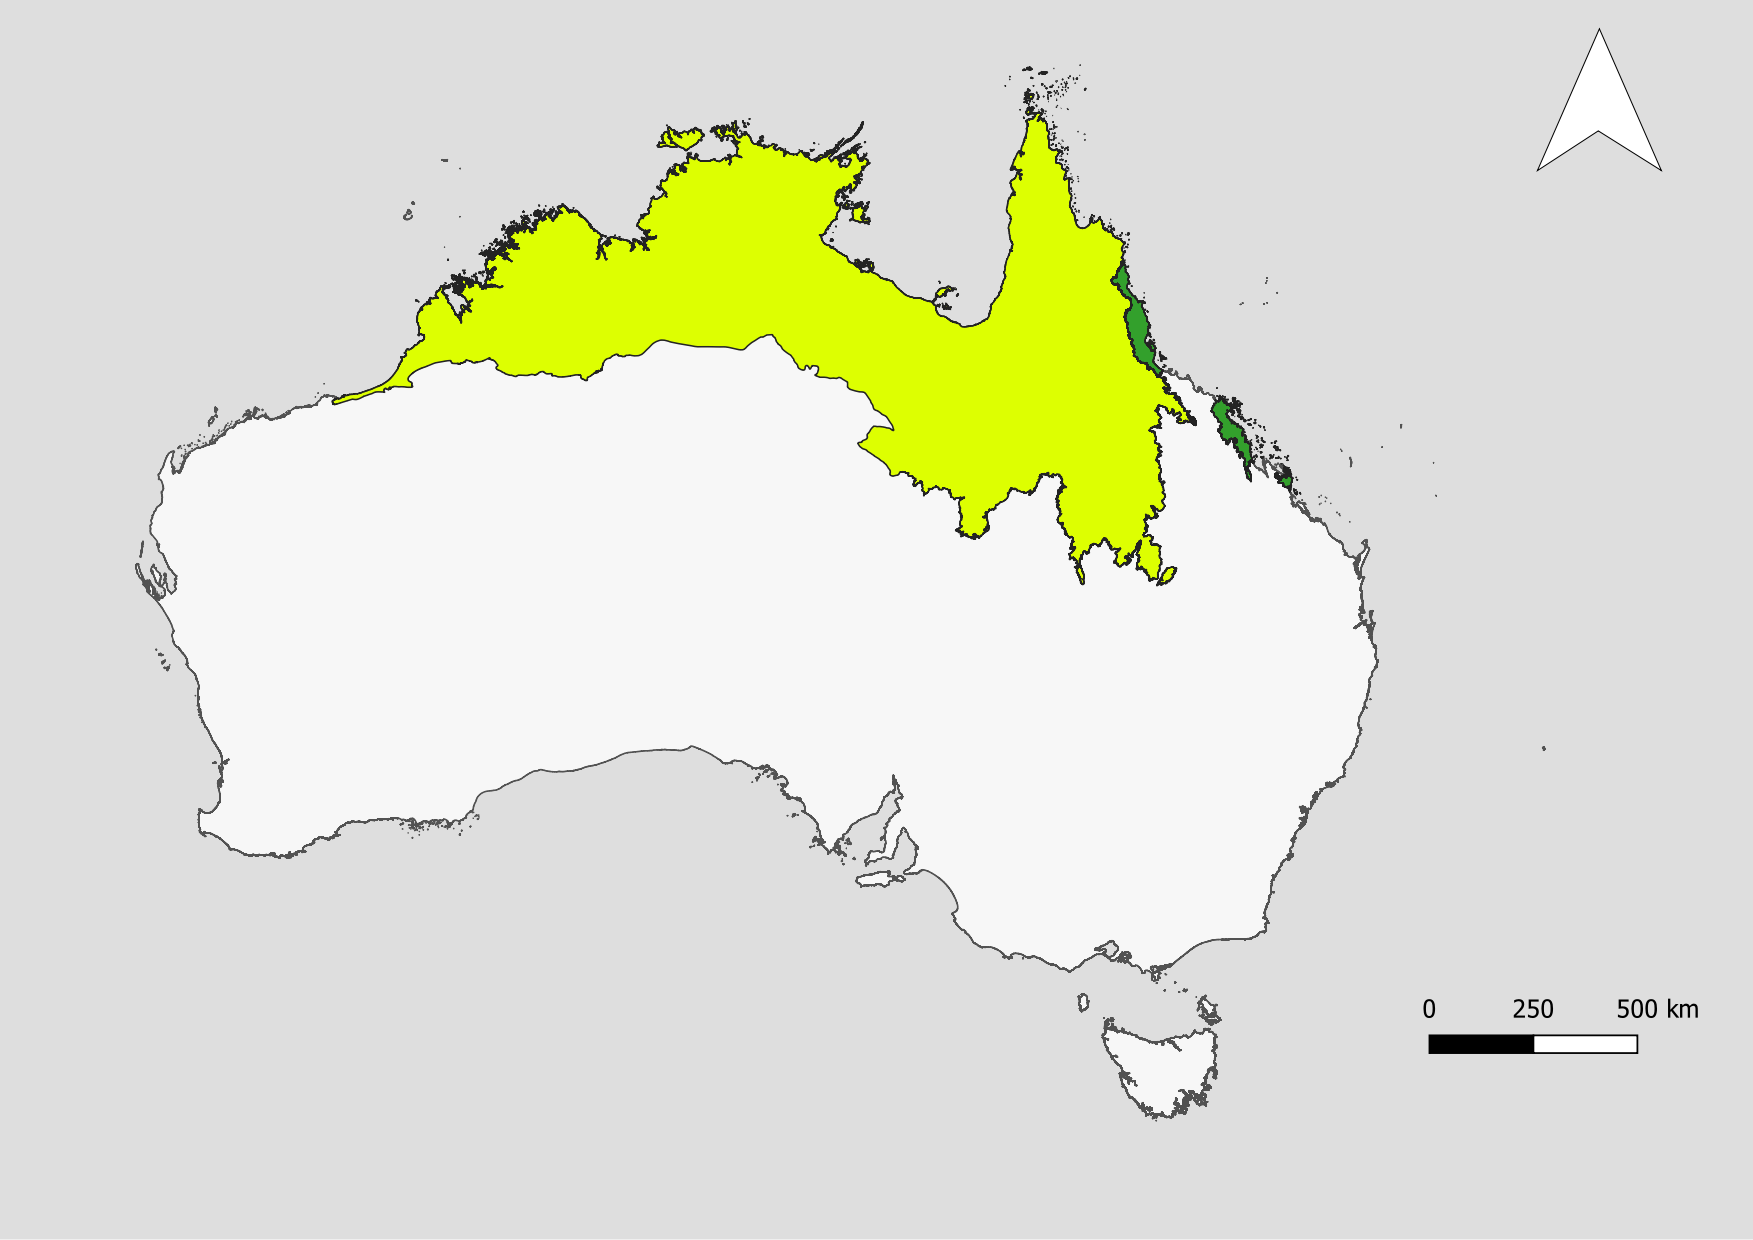
\includegraphics[width=0.8\linewidth]{C:/Users/Maria Jose Rivera/Documents/PhD/Figs/savannas_wet_AU} 

}

\caption{Location of tropical savannas in Australia (yellow) and wet tropics (green) (based on \citet{dinersteinEcoregionBasedApproachProtecting2017})}\label{fig:savanna}
\end{figure}



\hypertarget{organization-of-the-thesis}{%
\section{Organization of the Thesis}\label{organization-of-the-thesis}}

This thesis is organised according to the aims presented above. After the introductory first chapter, the second chapter presents the specific methodologies and workflow used in this PhD project, along with a general description of the study area and site. In addition, chapter 2 presents a literature review of the current knowledge of past climate, vegetation and fire on Cape York Peninsula in Australia. In the third chapter, the sedimentology and stratigraphy of the Sanamere sediment core is described, and this forms the foundation for the subsequent chapters. The fourth chapter addresses Aim I and contains the results of a comparison of several carbon fractions and pretreatments to determine the most reliable chronology for Sanamere Lagoon. Chapter 5 analyses the changes in climate and hydrologic conditions inferred from the lagoon sediment proxy records, while chapter six describes the vegetation and fire history of the area. Chapter 7 discusses the implications of the findings from chapters three to six and provides suggestions for future work (Figure \ref{fig:flow1}). Each chapter includes a chapter summary at the end to facilitate the reading.

\begin{figure}

{\centering 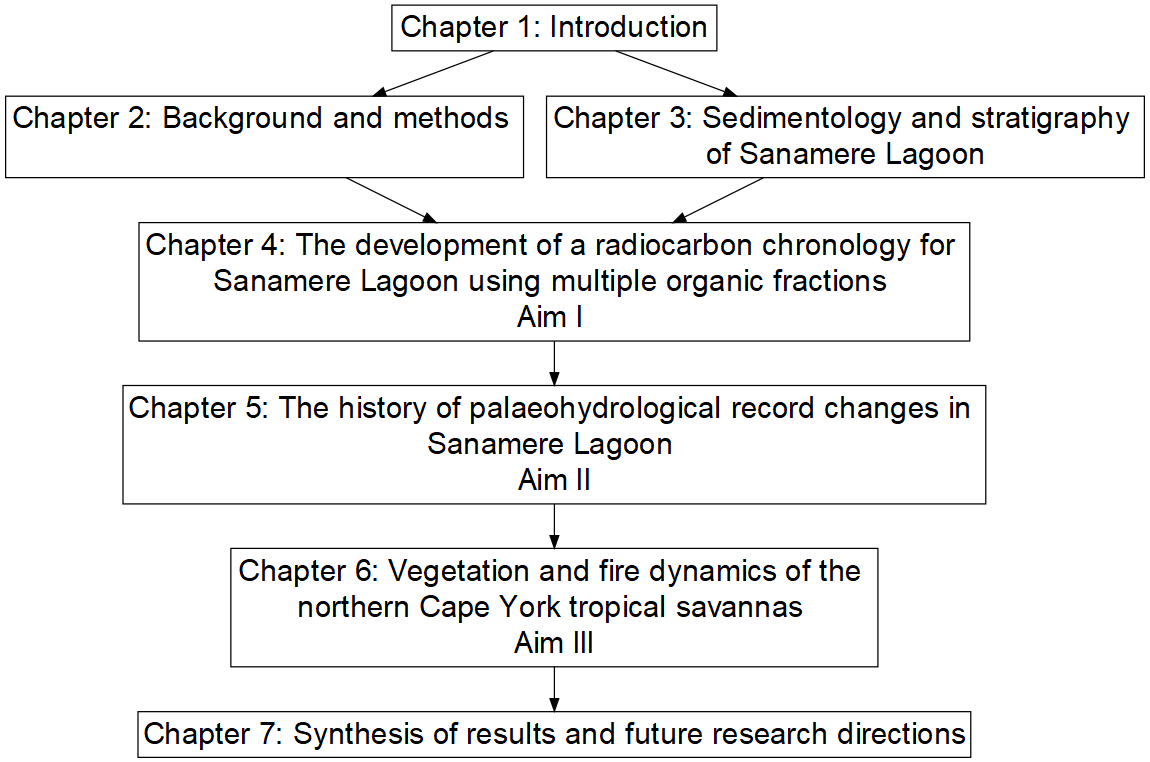
\includegraphics[width=0.8\linewidth]{C:/Users/Maria Jose Rivera/Documents/PhD/Figs/graphs_2} 

}

\caption{Flow chart of the thesis structure, linking thesis chapters to aims}\label{fig:flow1}
\end{figure}



\hypertarget{chapter-1-summary}{%
\section{Chapter 1 summary}\label{chapter-1-summary}}

Three basic aims are essential to understanding the environmental history of northern savannas of Cape York Peninsula: (1) Build a reliable chronology based on radiocarbon dating (2) Reconstruct the changes in palaeohydrology, and (3) Reconstruct the changes in vegetation and fire reflected at the site.

These aims elaborate upon two major themes: the standardisation of protocols to build radiocarbon dating chronologies and the understanding of past environmental changes. The research addresses these themes by analysing a lake sediment core from Sanamere Lagoon in Cape York Peninsula. Next, chapter 2 contextualizes the research question through a description of the study site and a review of the literature on past environmental change of Cape York, and the methodological perspectives that inform this research.

\hypertarget{background-and-methods}{%
\chapter{Background and methods}\label{background-and-methods}}

This chapter includes a description of the study area and its modern and past climatic contexts. In addition, it introduces the methods used in the development of this thesis, following the two main components (geochronology and environmental change).

\hypertarget{study-area}{%
\section{Study area}\label{study-area}}

Cape York Peninsula is located at the northernmost point of Queensland on the north-eastern coast of Australia. It lies between 10°S and 16°S and is one of the monsoonal regions of Northern Australia, along with the Kimberley and the Top End (Arnhem Land). Most of the Peninsula has a strongly seasonal tropical climate (tropical savanna) \citep{peelUpdatedWorldMap2007} with just a small area of wetter Am (tropical monsoon) environment on the eastern coast \citep{peelUpdatedWorldMap2007}. Annual rainfall varies from 800 mm in the central-southern part to over 2000 mm near the Iron Range (Figure \ref{fig:fig-cli-CP}). Approximately 80\% of the average annual rainfall falls during the four months from December to March. Temperatures are generally warm to hot, with maximum temperatures being over 40 °C in summer \citep{environmentscienceservicesStageOverviewReports1995}.

The vegetation of Cape York Peninsula is dominated by \emph{Eucalyptus} spp. woodlands, open woodlands, and open-forests, which occupy 64 \% of the area. The next most extensive vegetation group is the low open-woodlands, low woodlands, and tall shrublands, dominated by \emph{Melaleuca} spp. (14.2 \% of total area). Grasslands (6.1 \%), rainforests (5.6 \%) and heathlands (3.3 \%) are the next most extensive vegetation types \citep{neldnerVegetationSurveyMapping1995, foxVegetationAustralianTropical2001} (Figure \ref{fig:fig-veg-CP}).

The region has an abundance of internationally and nationally important natural resources, including remnant rainforests, rich mineral reserves (bauxite, gold, kaolin, silica sand), and several rivers of high ecological significance, high biodiversity, and a strong Indigenous culture \citep{hitchcockNaturalAttributesWorld2013}.

\begin{figure}

{\centering 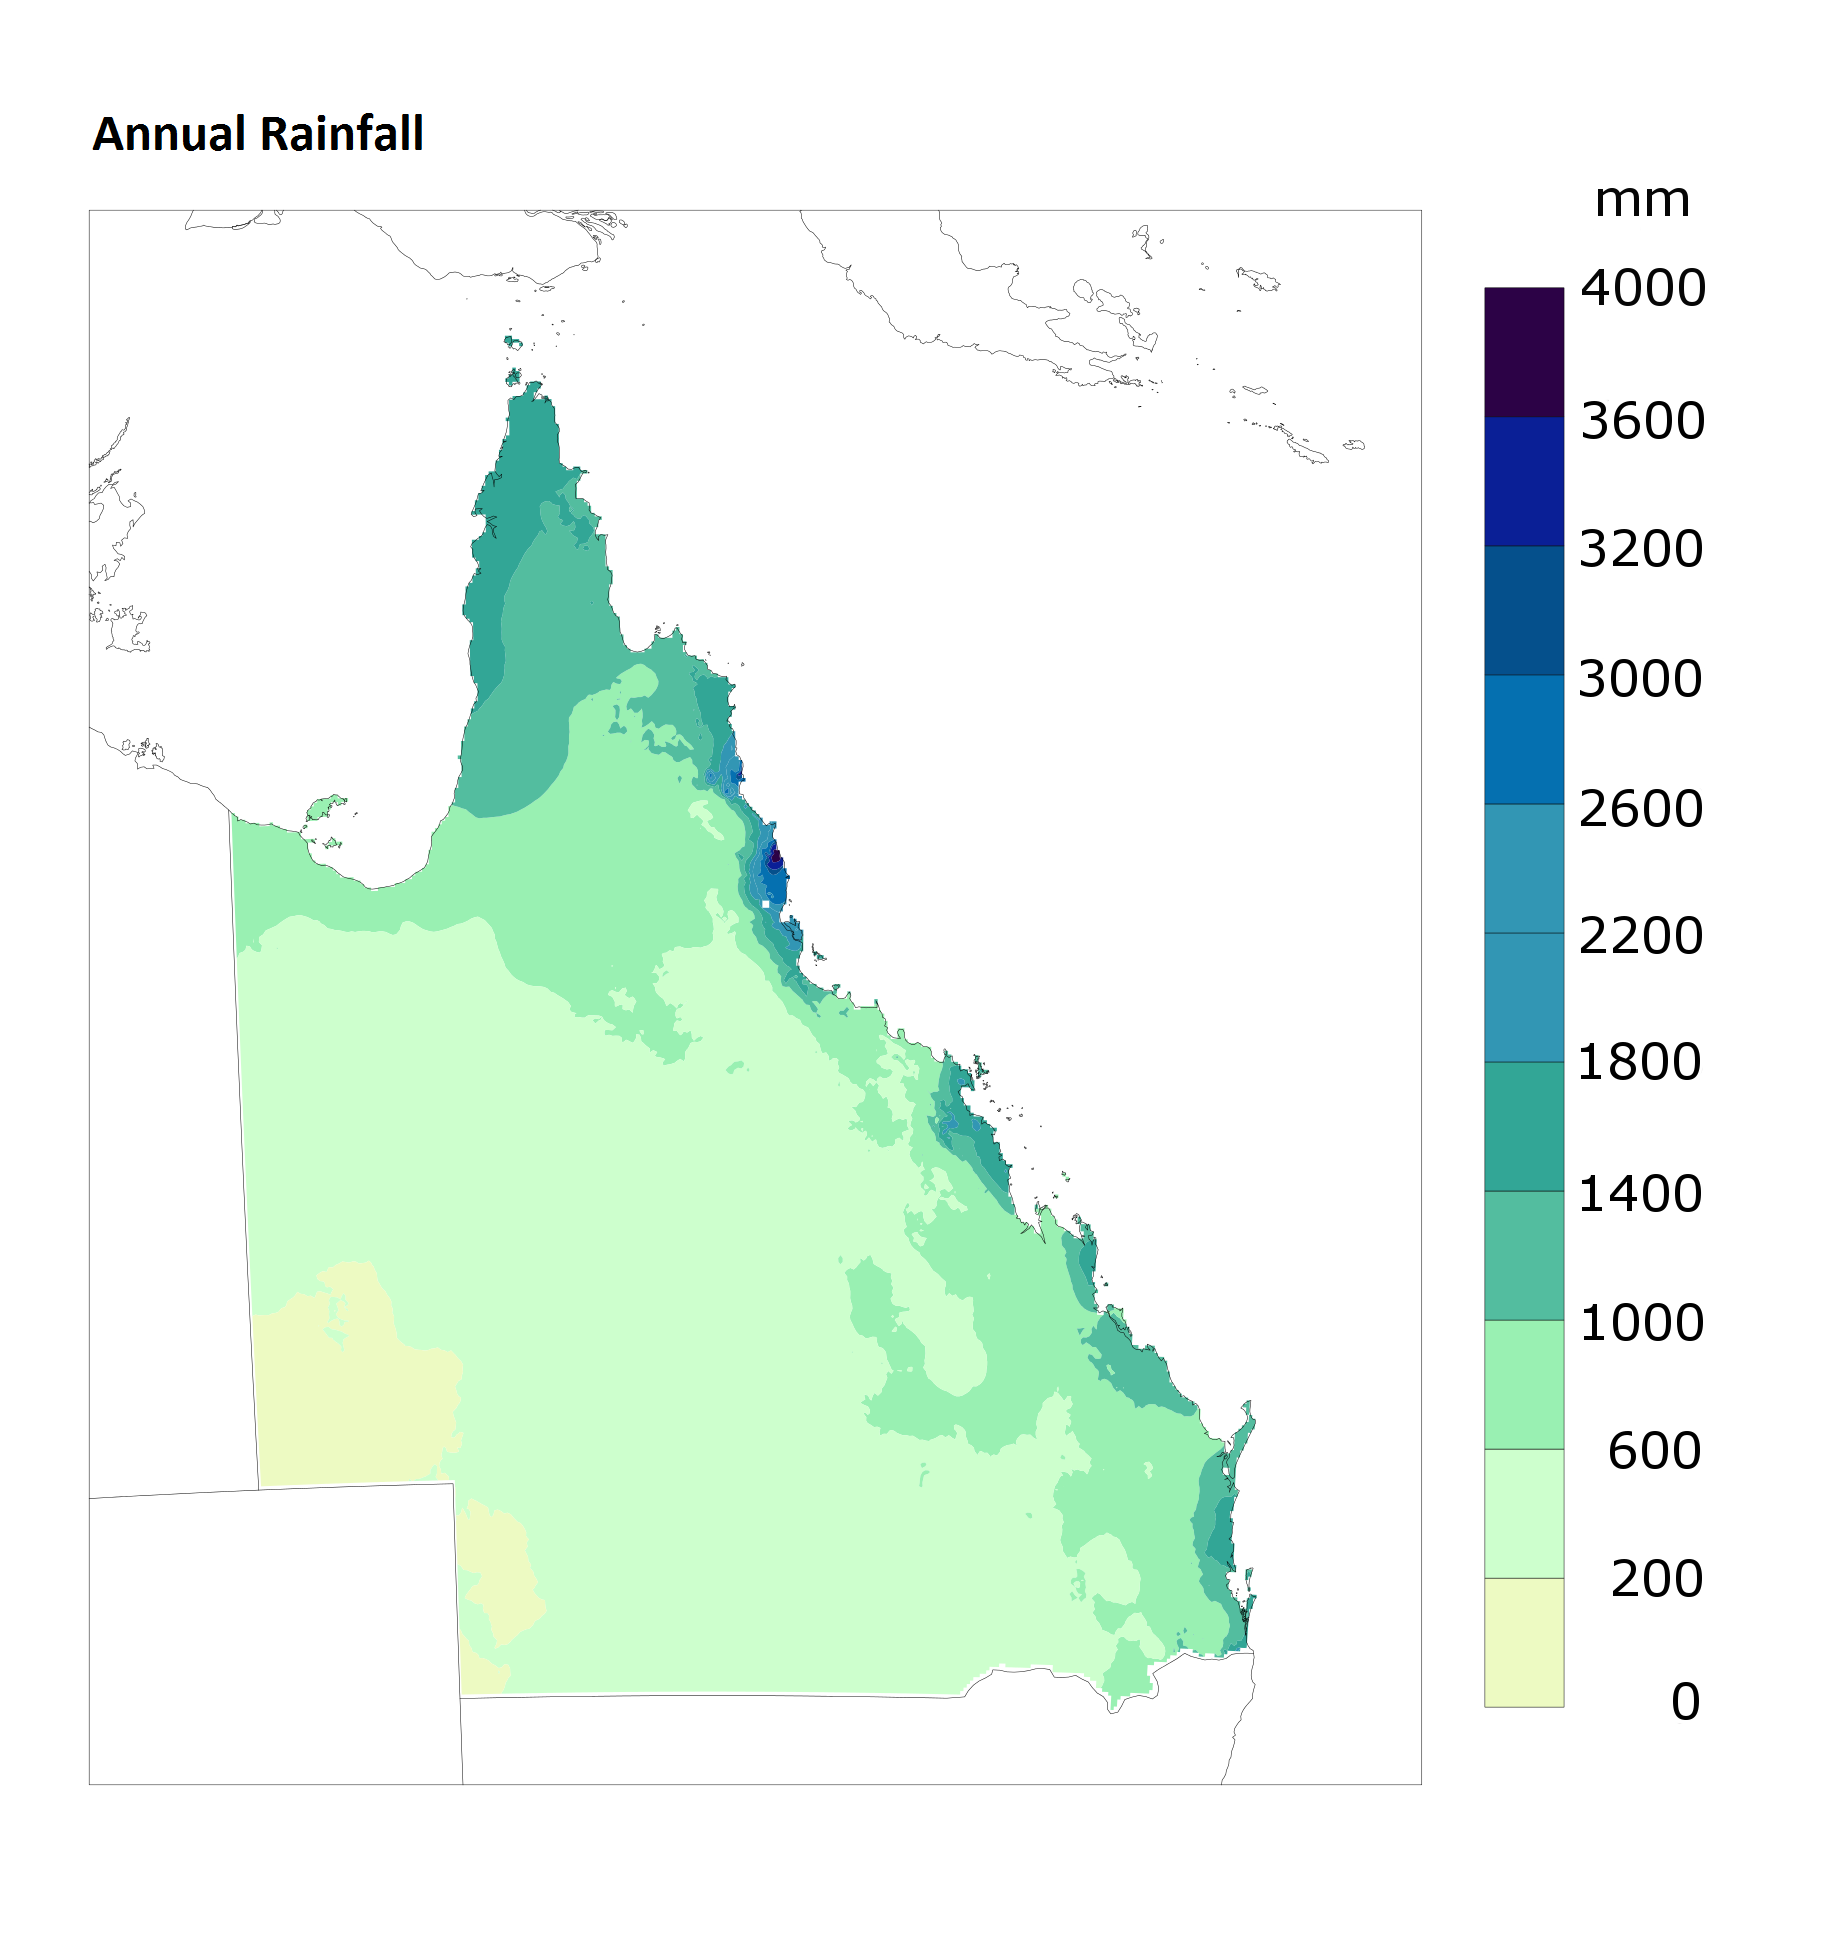
\includegraphics[width=0.8\linewidth]{C:/Users/Maria Jose Rivera/Documents/PhD/Figs/Background/CP_rainfall} 

}

\caption{Average annual rainfall, 2012--2016. Source: Bureau of Meteorology Australian Water Availability Project gridded monthly data. Plotted by the Queensland Government Department of Environment and Science. Available at \url{https://www.stateoftheenvironment.des.qld.gov.au/climate/climate-observations/annual-rainfall}}\label{fig:fig-cli-CP}
\end{figure}



\begin{figure}

{\centering 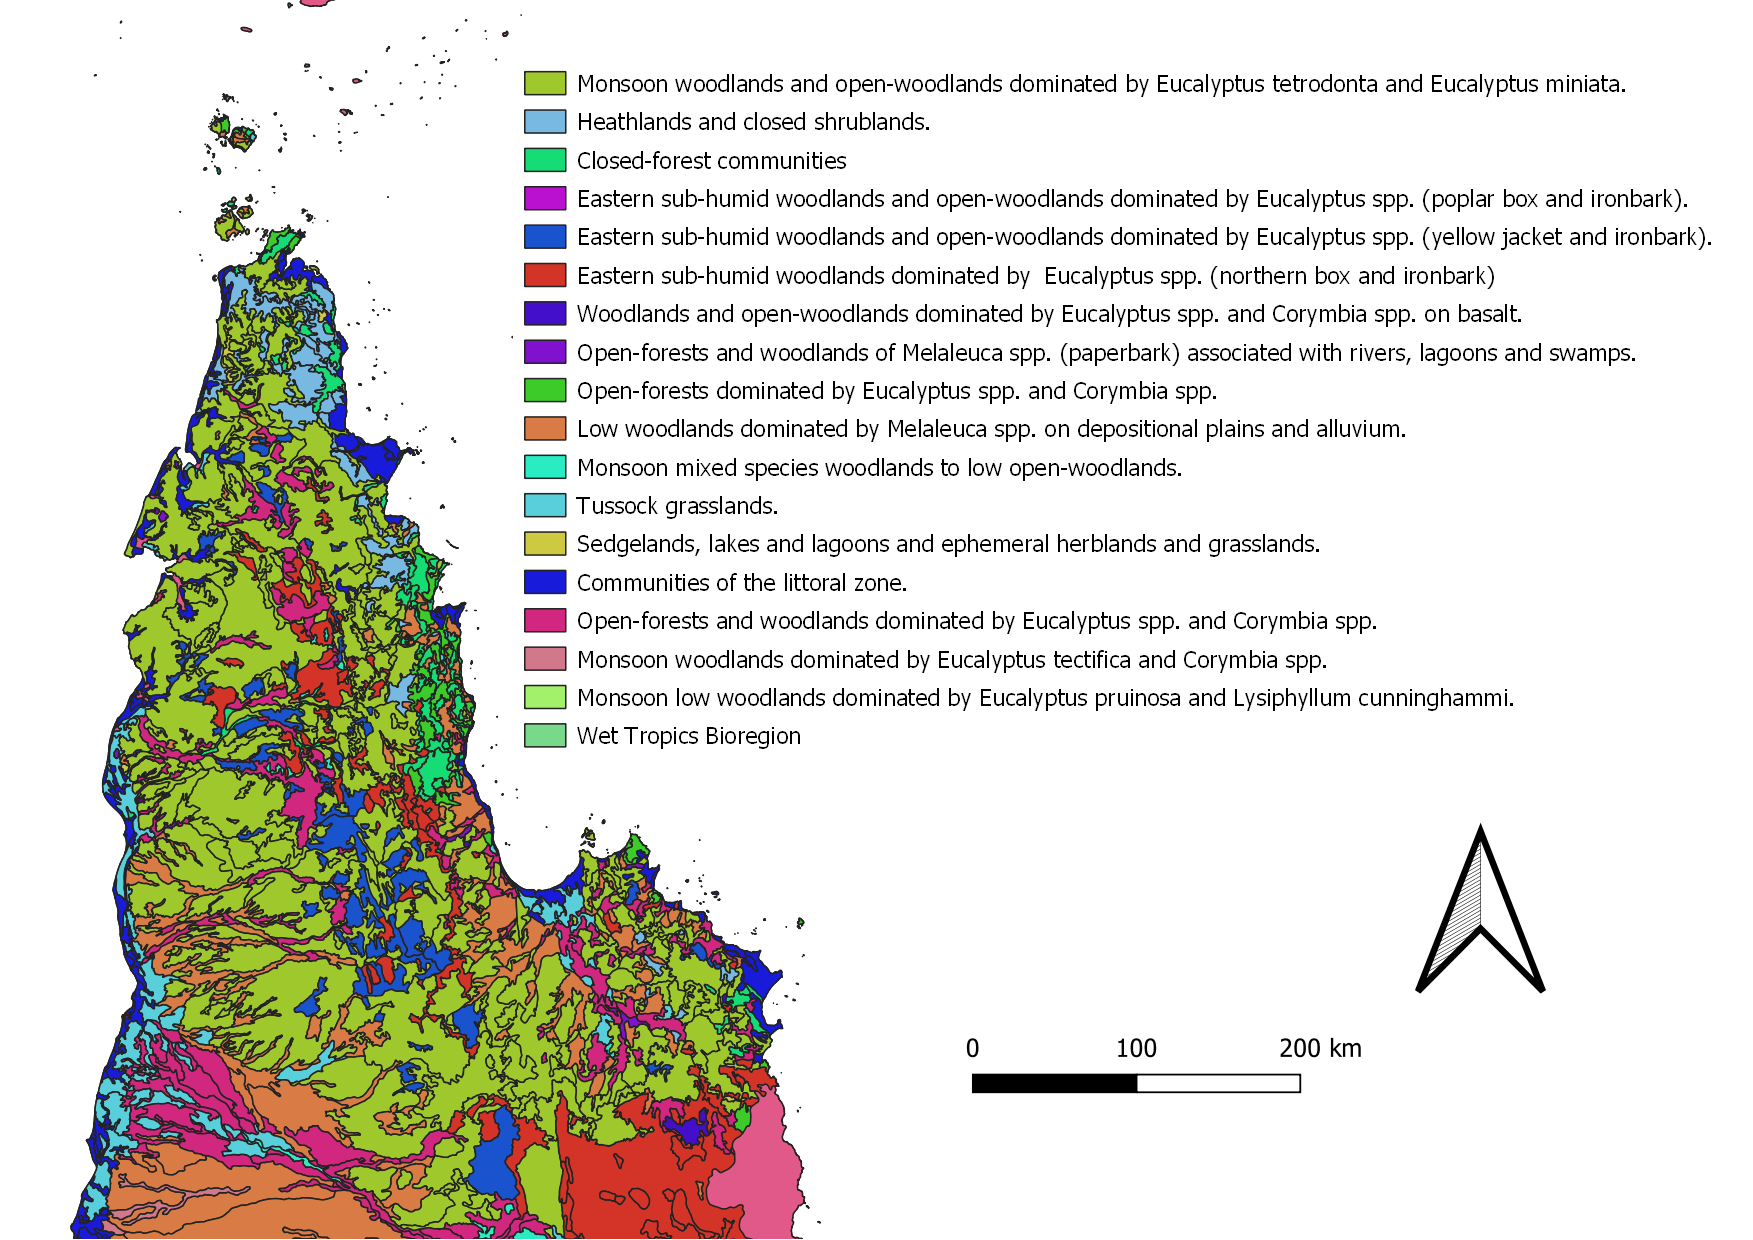
\includegraphics[width=0.8\linewidth]{C:/Users/Maria Jose Rivera/Documents/PhD/Figs/Background/CP_veg} 

}

\caption{Cape York Peninsula vegetation}\label{fig:fig-veg-CP}
\end{figure}



\hypertarget{study-site}{%
\section{Study site}\label{study-site}}

Sanamere Lagoon (11.123°S 142.359°E; 15 m asl) is located close to the northern tip of Cape York Peninsula and is part of the Apudthama Land Trust Area, classified as Aboriginal Freehold land and managed under the Northern Peninsula Area Regional Council. The lagoon is 1 km north of the W-E flowing perennial Jardine River (Figure \ref{fig:fig-jardine}). The climate of the region is monsoonal with 88 \% of the annual 1753 mm rainfall falling between December and April with a mean annual temperature of 27 °C \citep{bomMonthlyClimateStatistics2018}. Winds are predominantly from the north-northwest and southeast in January and July, respectively \citep{bomRoseWindDirection2019} (Figure \ref{fig:fig-wind-SAN}). Sanamere Lagoon is considered a sub-coastal wet heath swamp, and a palustrine system (a wetland with more than 30 \% emergent vegetation) \citep{departmentofenvironmentscienceWetlandInfoWetlandSystems2018}. Sanamere Lagoon is also referred as of value as a ``wilderness wetland area'' \citep{abrahamsAreasConservationSignificance1995}. The Anggamudi (also known as Angkamuthi), Wuthahti (alternatively Wuthathi) and Yadhaigana (alternatively Yadhaykenu) people are the traditional owners of the Jardine River catchment {[}australianinstituteofaboriginaltorresstraitislanderstudiesAIATSISCollection2020{]}.

Although most lakes dry out in this region during the dry season (May - November), the Water Observations from Space (WOfS) dataset \citep{muellerWaterObservationsSpace2016, commonwealthofaustraliaUnfilteredSummaryAll2018} indicates that the deeper parts of Sanamere Lagoon have been permanently covered by standing water for the last 35 years, despite periods of significantly below average rainfall in this period (Figure \ref{fig:fig-water-SAN}). The water depth during the dry season is 1.2 m for most of the lake. At this level, several relict dune features are exposed, dating from the time of lagoon impoundment. The lake was probably formed as a result of the collapse of laterite karst to form a sinkhole-like depression below the local water table \citep{grimes2008laterite}. During the wet season, the dune features are largely submerged and the lake outflows into the Jardine River.

Sanamere is in an enclosed basin surrounded by higher elevation land, with the highest point (57 m a.s.l.) to the north-northeast of the lagoon, close to the current Bamaga Road \citep{geoscience-australiaSRTMSecImage2015}. Based on topography, Sanamere Lagoon has an approximate catchment area of 9 km\textsuperscript{2}, with the lowest overflow point at \textasciitilde17 m a.s.l. to the west of the lagoon (Figure \ref{fig:fig-DEM-SAN}).

\begin{figure}

{\centering 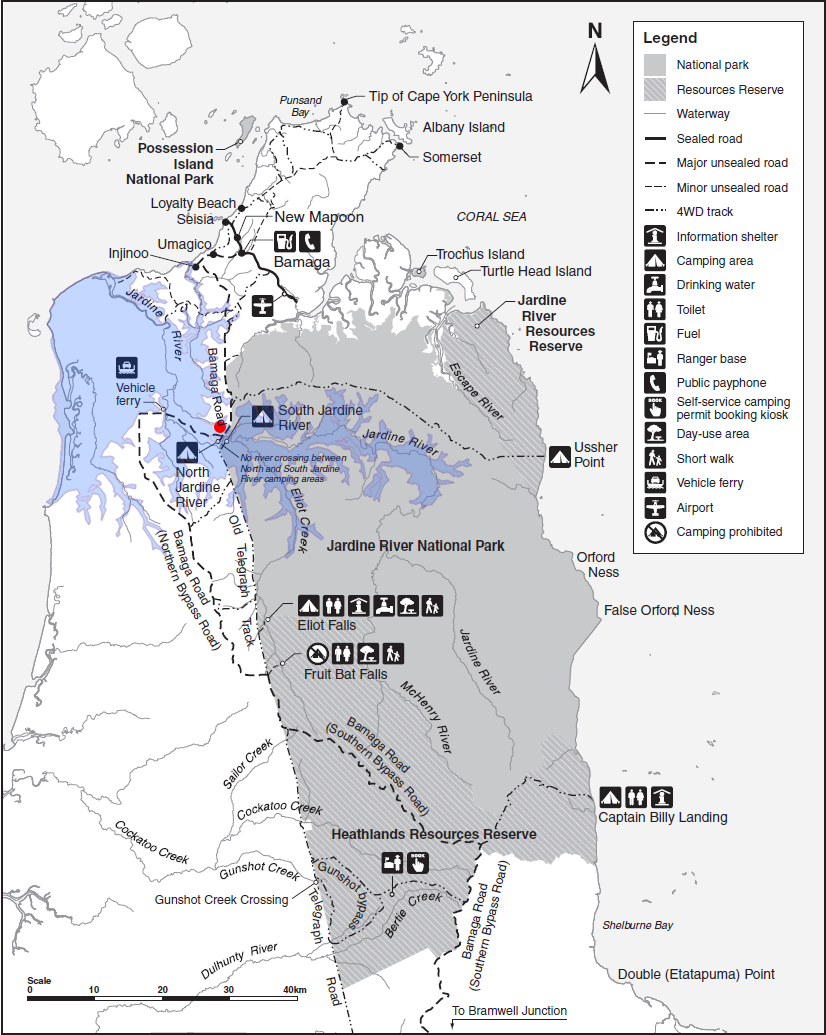
\includegraphics[width=1\linewidth]{C:/Users/Maria Jose Rivera/Documents/PhD/Figs/Background/Jardine} 

}

\caption{Map of the Jardine River National Park, Jardine River Resources Reserve and Heathland Resources Reserve, with Sanamere indicated in red and the Jardine River Wetlands Aggregation shaded blue (courtesy of Emma Rehn).}\label{fig:fig-jardine}
\end{figure}



\begin{figure}

{\centering 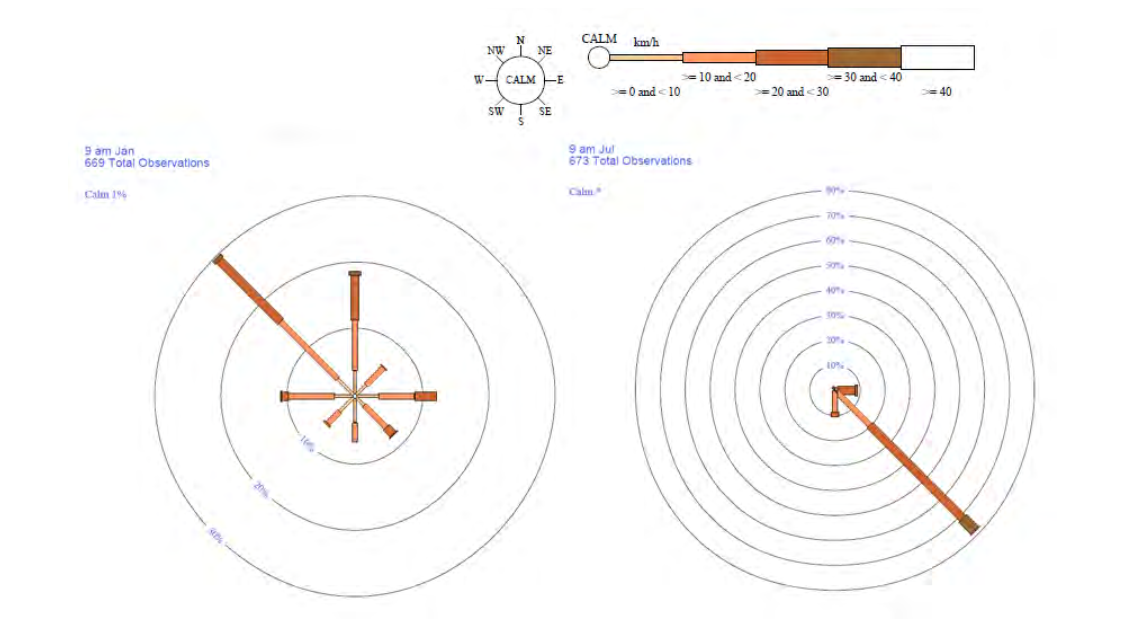
\includegraphics[width=0.8\linewidth]{C:/Users/Maria Jose Rivera/Documents/PhD/Figs/Background/horn_wind} 

}

\caption{Average wind direction and speed 1995-2017, measured at 9 am in in January (left) and July (right), from Horn Island weather station.}\label{fig:fig-wind-SAN}
\end{figure}



\begin{figure}

{\centering 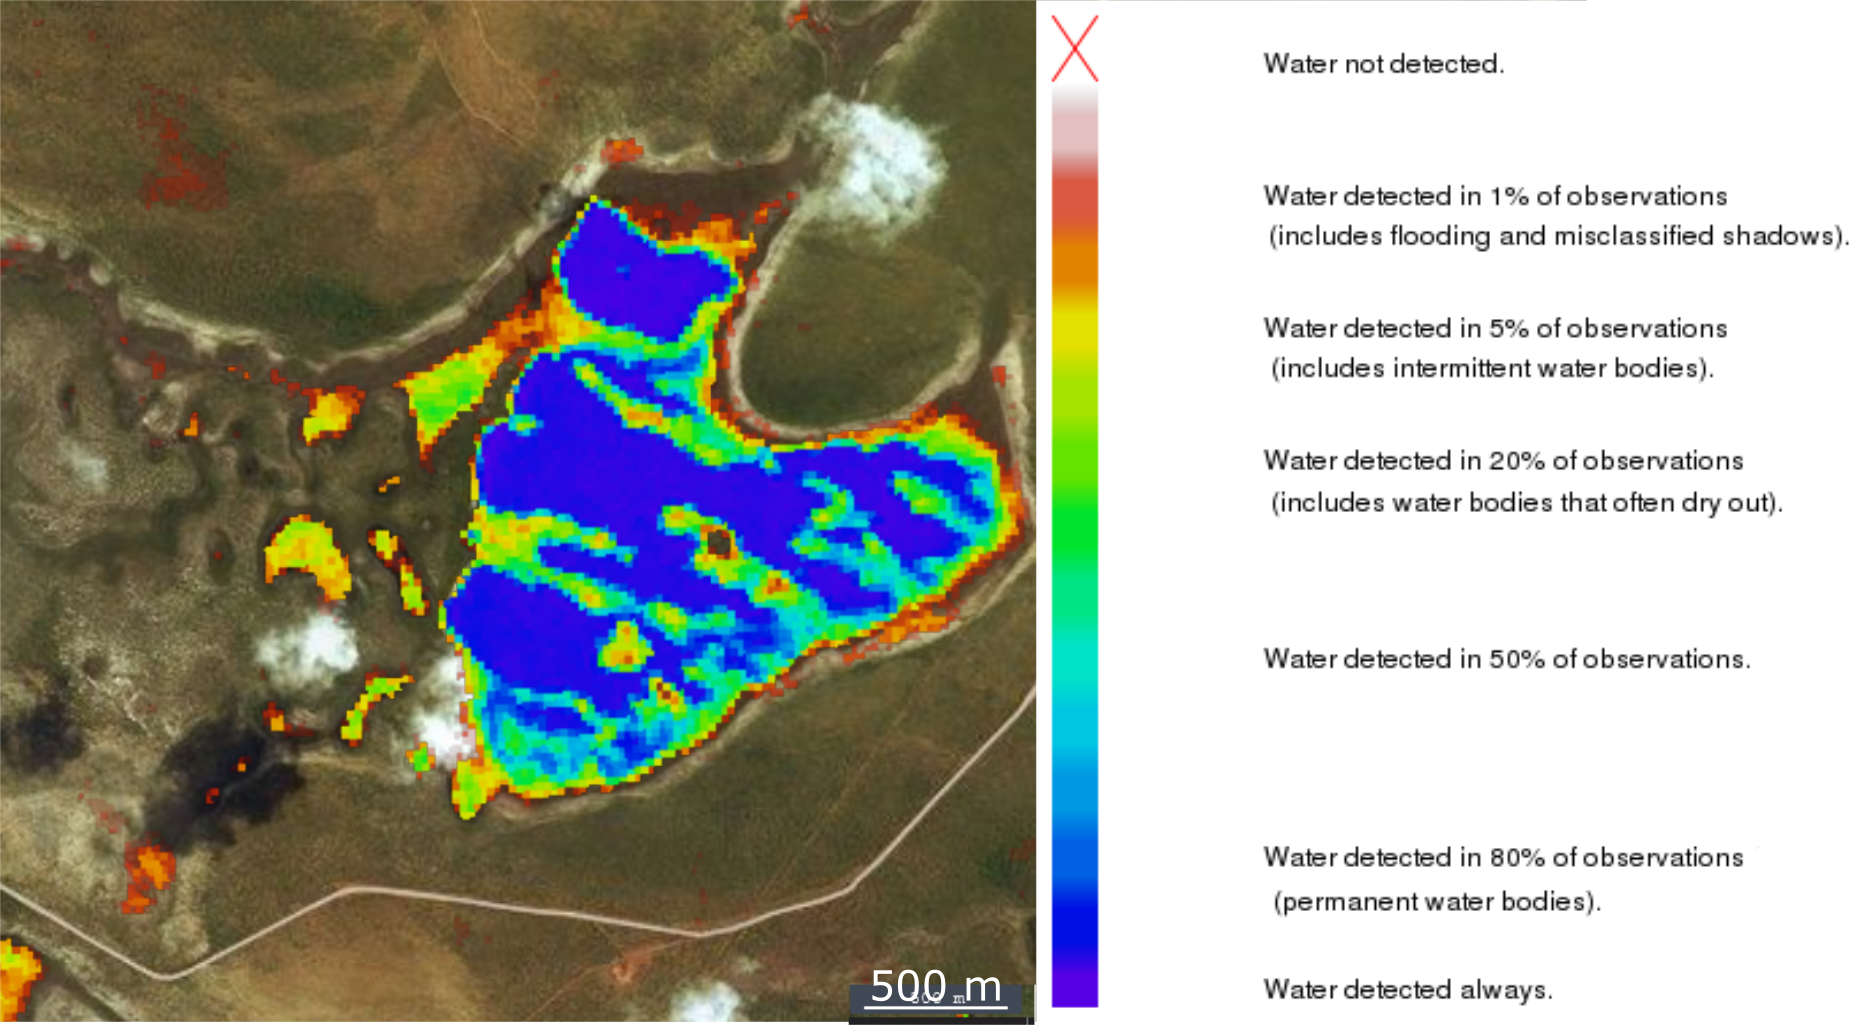
\includegraphics[width=0.8\linewidth]{C:/Users/Maria Jose Rivera/Documents/PhD/Figs/Background/water_SAN} 

}

\caption{WOfS data showing permanency of water in the lagoon since 1986 with blue denoting areas permanently covered, possible relict dune features shown as low permanency areas, exposed in the dry season}\label{fig:fig-water-SAN}
\end{figure}



\begin{figure}

{\centering 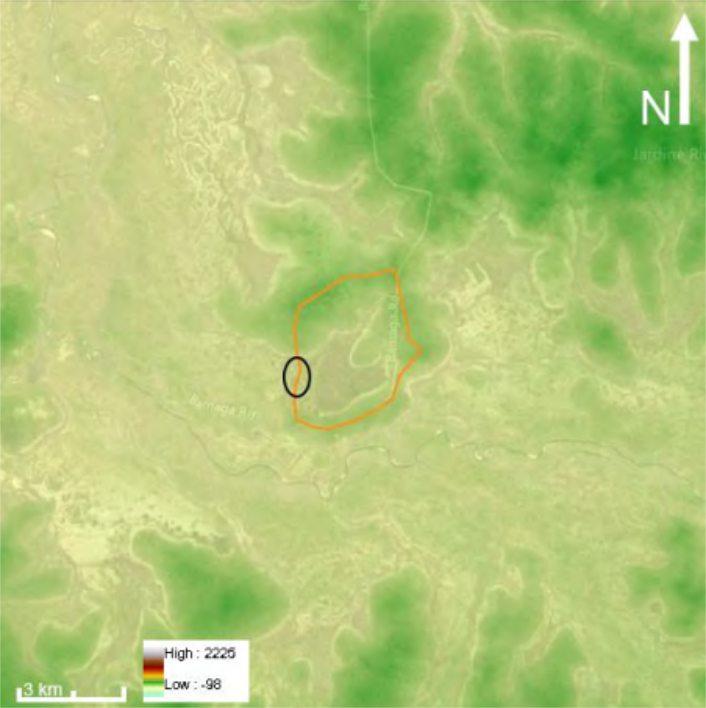
\includegraphics[width=0.8\linewidth]{C:/Users/Maria Jose Rivera/Documents/PhD/Figs/Background/DEM_SAN} 

}

\caption{Digital elevation map of Sanamere Lagoon and surrounds, with the approximate catchment area of the lagoon marked in orange and western low point (outlet) circled in black. Darker green indicates higher elevation (diagram courtesy of Emma Rehn).}\label{fig:fig-DEM-SAN}
\end{figure}



\hypertarget{geology-and-lake-formation}{%
\subsection{Geology and lake formation}\label{geology-and-lake-formation}}

The geology of the watershed is represented by middle Jurassic to Early Cretaceous Helby Beds (Geology 1:250,000 sheet SC54-15)\citep{AustralianGeoscienceInformation2020}, which are composed by clayey quartzose sandstone and pebble conglomerate, not underlain by carbonate-bearing lithologies. The lake is likely to have formed by a collapse into cavities formed by dissolution of underlying rock and it is an example of `laterite karst' \citep{grimes2008laterite}.

\hypertarget{veg}{%
\subsection{Vegetation}\label{veg}}

The vegetation around the lake edge is dominated by sedgeland, open-heaths, dwarf open-heaths and woodlands. Between the edge and 50 m sedges such as \emph{Eleocharis sphacelate} dominate the landscape (Figure \ref{fig:fig-veg2}). Between 50 m and 300 m vegetation transitions to open heath and shrubland, which then account for most plant species, \emph{Neofabricia}, \emph{Asteromyrtus}, \emph{Baeckea}, \emph{Jacksonia}, \emph{Hibbertia}, \emph{Thryptomene}, \emph{Allocasuarina} and \emph{Grevillea} (Figure \ref{fig:fig-veg1}). At 300 m from the lake there is another transition to \emph{Eucalytus} woodlands, especially \emph{Eucalyptus tetrodonta} (Figure \ref{fig:fig-veg3}) \citep{neldnerVegetationSurveyMapping1995}. Smaller sub-canopy trees are common and include \emph{Acacia}, \emph{Grevillea glauca} and \emph{Grevillea pteridifolia} as well as \emph{Livisonia} palm, with \emph{Asteromyrtus} present as shrub. \emph{Banksia} and \emph{Casuarina} are present in wetter low-lying areas. Grasses dominate the ground cover in this area (Poaceae) and leaf litter is greater than that found in the heathland.



\begin{figure}

{\centering 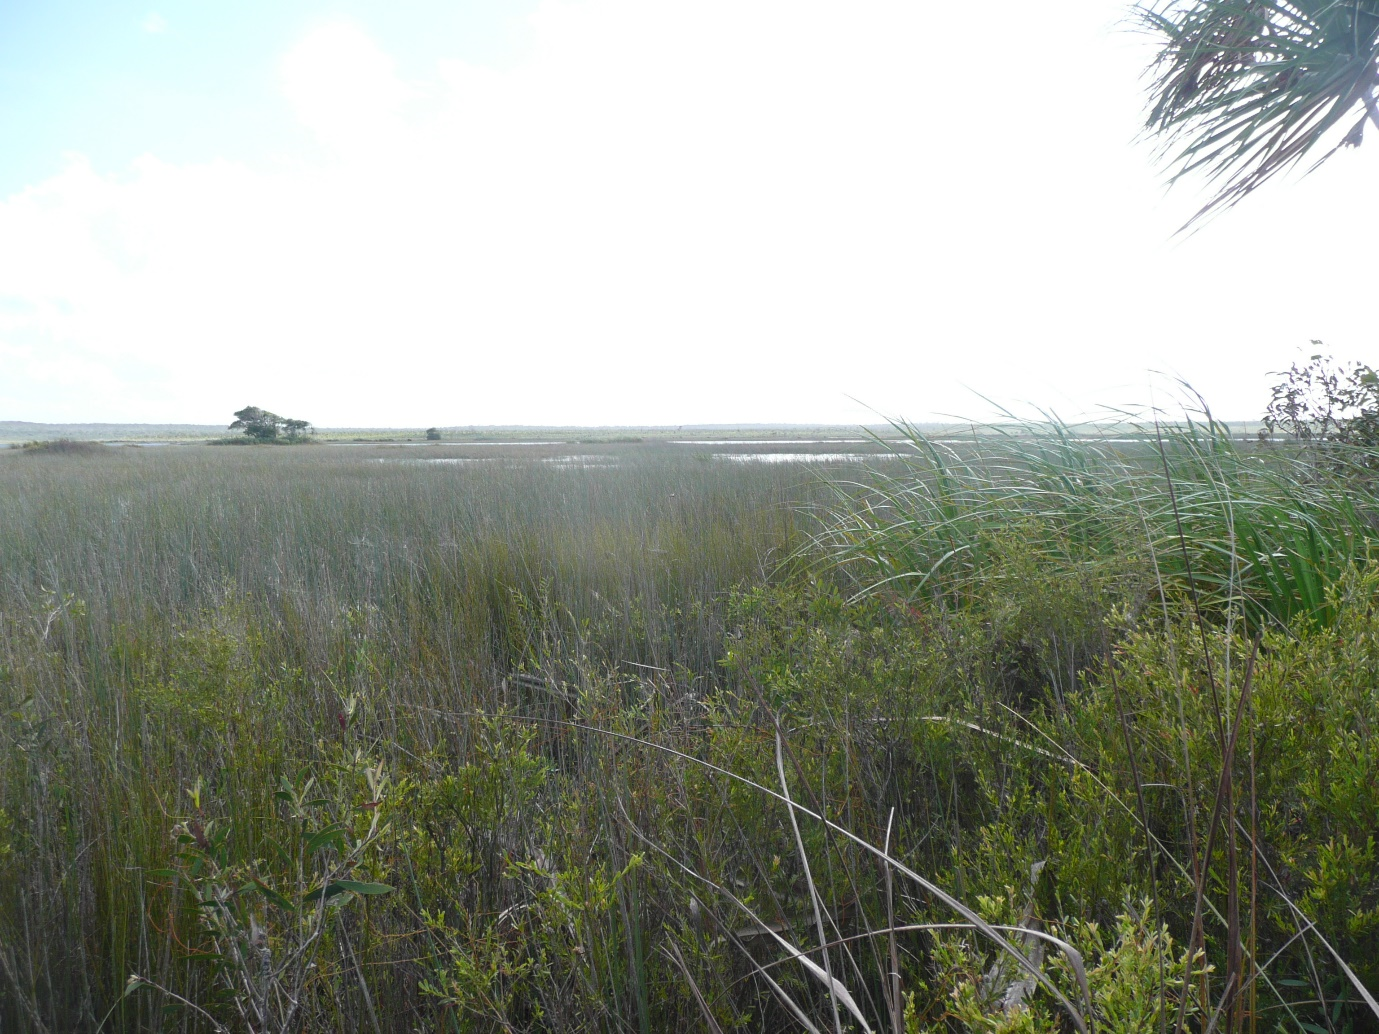
\includegraphics[width=1\linewidth]{C:/Users/Maria Jose Rivera/Documents/PhD/Figs/vegetation/0_waterline} 

}

\caption{Vegetation at the Sanamere Lagoon waterline, comprised of sedges and scattered Pandanus}\label{fig:fig-veg2}
\end{figure}



\begin{figure}

{\centering 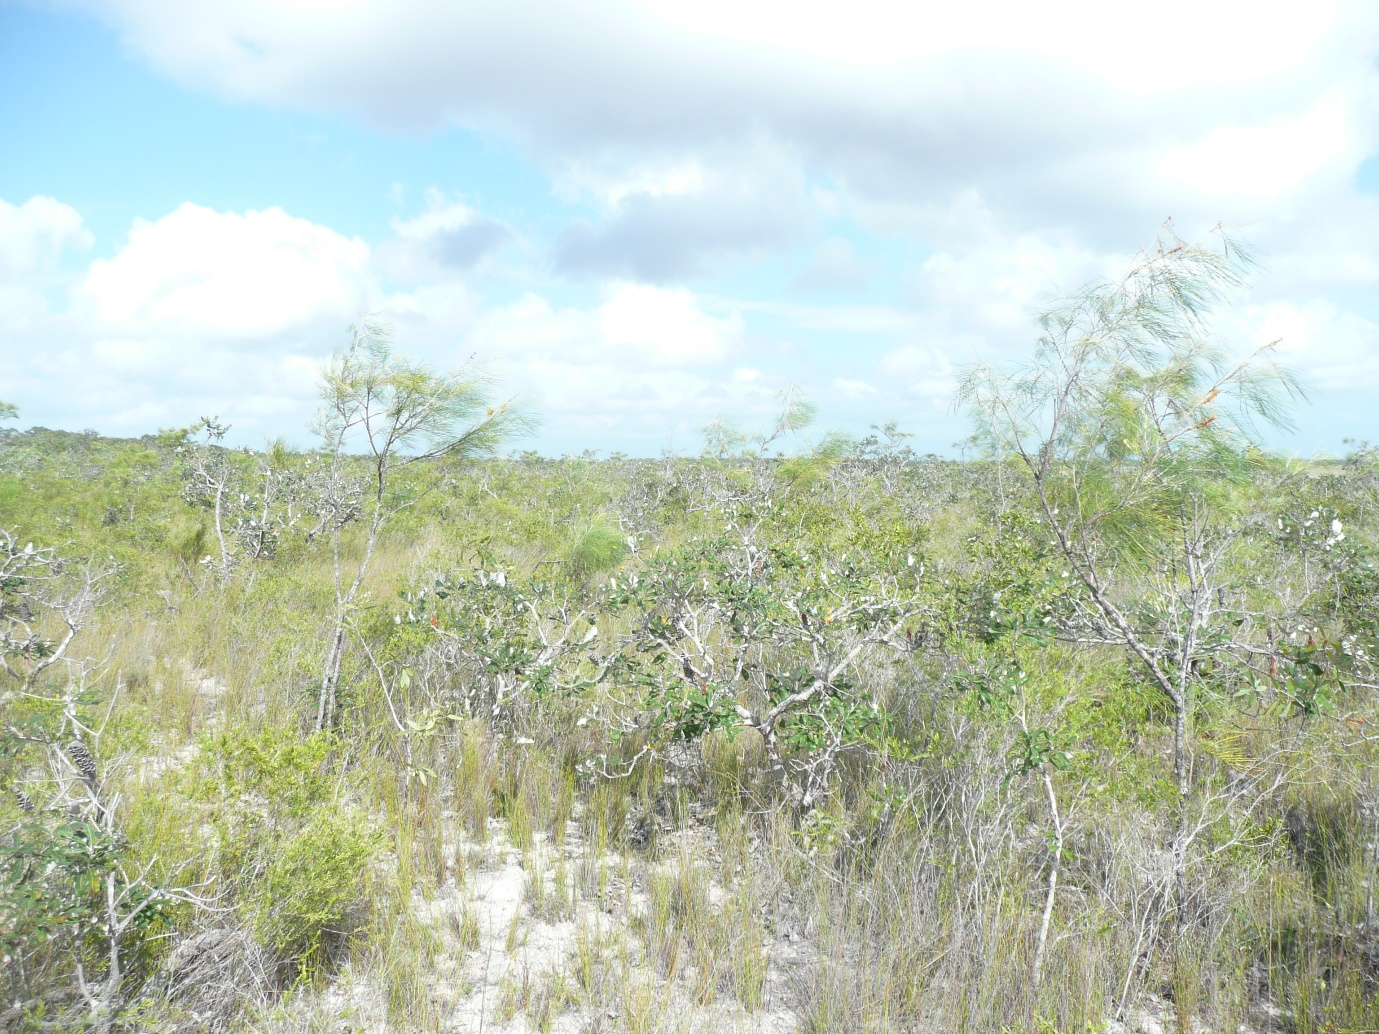
\includegraphics[width=1\linewidth]{C:/Users/Maria Jose Rivera/Documents/PhD/Figs/vegetation/0_50_heathland} 

}

\caption{Open heathland vegetation 50 metres from the waterline}\label{fig:fig-veg1}
\end{figure}



\begin{figure}

{\centering 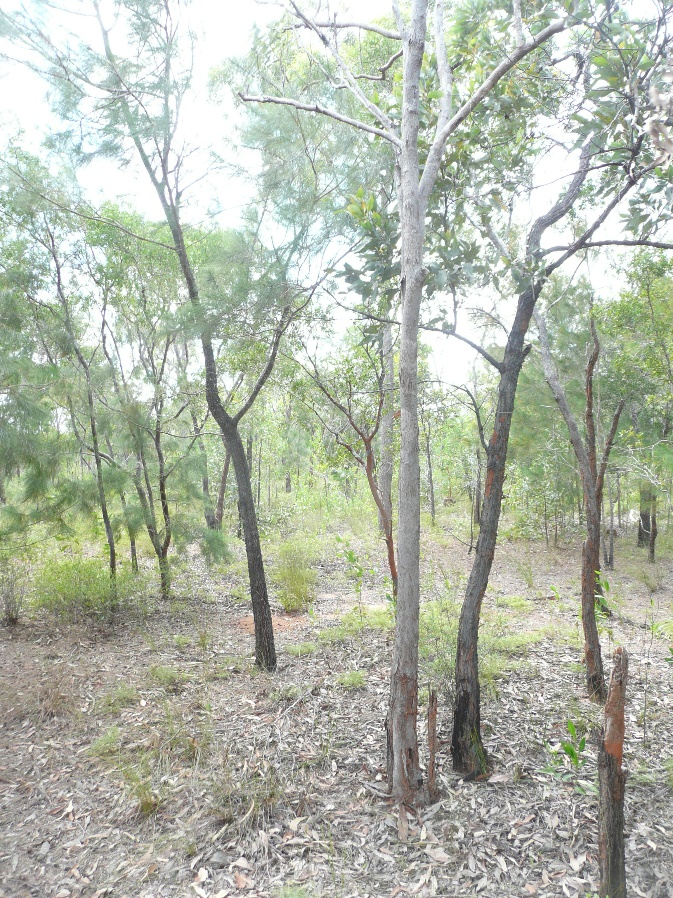
\includegraphics[width=1\linewidth]{C:/Users/Maria Jose Rivera/Documents/PhD/Figs/vegetation/400_Eucalyptus} 

}

\caption{Eucalyptus woodland at 400 m (right) from the waterline}\label{fig:fig-veg3}
\end{figure}



\hypertarget{soils}{%
\subsection{Soils}\label{soils}}

Sanamere's catchment is characterized by deep bleached uniform yellow earthy sands with poor drainage, flooding and low fertility. Soils are primarily derived from sandstone (Kandosols and Tenosols) \citep{biggsSoilsCapeYork1995}. Tenosols on undulating rises of sandstone comprise the largest unit within the Heathlands Landscape. Both the Kandosols and Tenosols are infertile.

\hypertarget{fire}{%
\subsection{Fire}\label{fire}}

Northern Australia is the most fire‐prone area of Australia, with around 250,000--450,000 km\textsuperscript{2} burnt each year \citep{russell-smithFireManagementBusiness2016}. Australian savannas are characterized by low nutrient soils, highly connected landscapes with few topographic barriers that help generate fire regimes of frequent, intense and large fires \citep{stevensSavannaWoodyEncroachment2017}. These fires are one of the main drivers of vegetation dynamics and climate in the area. For example, the role of fire in controlling the balance between grasses and woody vegetation in savannas have been widely studied \citep{lehmannDecipheringDistributionSavanna2011}, and most literature suggests that frequent fire reduces woody growth rates and tree density, and creates an environment more suitable for C\textsubscript{4} grasses \citep{lehmannDecipheringDistributionSavanna2011}. However, recent studies debate the role of fire regimes to reduce canopy vegetative cover and argue that this role is much more limited in impact than often assumed \citep{veenendaalRelationshipFireRegime2018}. In palaeoecological research, burning has also been related to the opening of woodland (canopy and subcanopy) and creating patches of different plant communities \citep{roweLateHoloceneSwamp2015}.

In the 18-year period spanning 2000-2019, the area immediately surrounding Sanamere Lagoon (catchment and beyond) burned on average every 3 to 7 years \citep{northaustraliarangelandsfireinformationData2020}. Fire scars recorded in this period over the surface of the lagoon (Figure \ref{fig:fig-fire-SAN}) are likely a result of error in the determination of fire scars \citep{rehnFireEnvironmentalChange2020}. However, fire scars that extend substantially beyond the water surface may be assumed to represent real scars.

Most fires occur each year during the later dry season (July - November). During April to July, fires in northern Australia are associated with lower air temperatures, higher moisture content, burning of smaller areas and may leave unburnt patches. Fires occurring between August and November are typically high intensity, and burn large areas \citep{evansDeliveringEffectiveSavanna2020}. Australian Aboriginal people have used fire to manage the landscape for millennia. However, in the early 20th century the removal of Indigenous people to missions might have reduced intensive management of fire regime {[}cookeCultureEcologyEconomy2009{]}.

\begin{figure}

{\centering 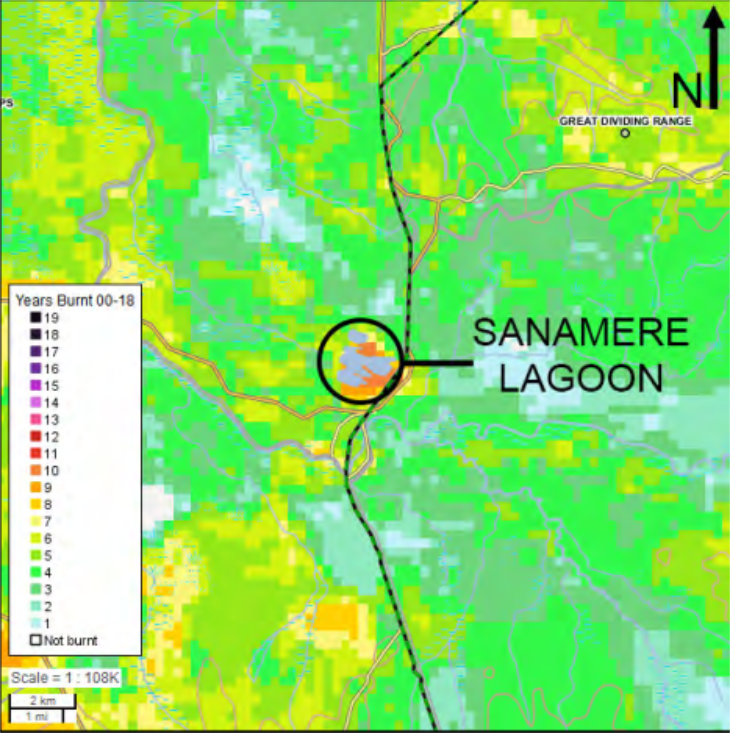
\includegraphics[width=1\linewidth]{C:/Users/Maria Jose Rivera/Documents/PhD/Figs/Background/fire_SAN} 

}

\caption{Number of years areas around Sanamere burned in the 10 years 2010 - 2018}\label{fig:fig-fire-SAN}
\end{figure}



\hypertarget{climatic-context}{%
\section{Climatic context}\label{climatic-context}}

\hypertarget{modern-climate}{%
\subsection{Modern climate}\label{modern-climate}}

The climate of the northeastern Australia's tropical savannas is largely determined by the annual movement of the monsoon system. Along with the monsoon, the southeasterly trade winds along the east coast during the dry season define most of the area \citep{shiClimateDataTheir2016}. The monsoons are active from about November to March and are followed by a distinct seasonal drought for the remainder of the year. Tropical cyclones that form over the adjacent ocean also influence the climate of the Peninsula and cause extreme episodic rainfall events during the wet season. The main driver of Australian rainfall variability is El Niño--Southern Oscillation (ENSO) in the Pacific Ocean \citep{risbeyRemoteDriversRainfall2009}. However, the Indian Ocean dipole (IOD) and Madden--Julian oscillation (MJO) also contribute to rainfall variability in northern Australia \citep{bomAustralianClimateInfluences2010}.

The influence of the monsoon is controlled by the position of the Intertropical Convergence Zone (ITCZ) and the Indo-Pacific Warm Pool (IPWP). Their impact in the climate system is determined by the oceanic circulation system. For instance, the Indo-Pacific Warm Pool provides a large moisture source for the Northwest Monsoon and is an important component of the coupled ocean-atmosphere processes that gives rise to the El Niño--Southern Oscillation (ENSO) \citep{kershawAustraliaSouthwestPacific2012}.

The monsoon system is divisible into three spatial components: the Northwest Monsoon that derives its moisture from the equatorial seas to the north and is considered to be `pushed' by the Asian winter monsoon; the Pseudo-Monsoon of northwestern Australia that is driven by moist winds emanating from the Indian Ocean; and the Quasi-Monsoon that derives much of its moisture from easterly Pacific Ocean winds \citep{gentilliClimatesAustraliaNew1971}. The Australian monsoon alternates between two seasonal phases linked to wind direction. In the winter phase, easterly trade winds bring dry conditions, and particularly the northern Australian region experiences an almost rainless dry season of about 7--8 months. In the summer, westerly winds bring sustained rainy conditions, torrential rains and, cyclones (Figure \ref{fig:fig-modern}).

\begin{figure}

{\centering 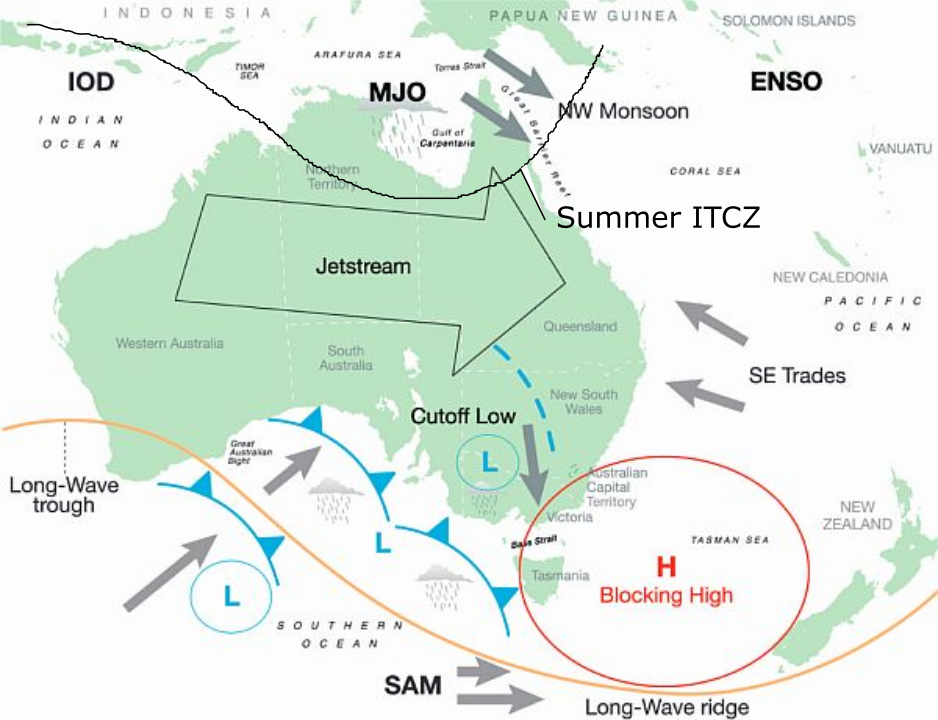
\includegraphics[width=0.8\linewidth]{C:/Users/Maria Jose Rivera/Documents/PhD/Figs/Background/climate_NA} 

}

\caption{Influences on modern Australian climate. Modified from \citet{risbeyRemoteDriversRainfall2009}. © American Meteorological Society. Used with permission.}\label{fig:fig-modern}
\end{figure}



\hypertarget{pastclimate}{%
\subsection{Past climate, vegetation and fire}\label{pastclimate}}

The following section summarises the current knowledge of past climate in the study area (covering \textasciitilde{} 800 km around the region), following the chronological divisions proposed by \citet{reevesPalaeoenvironmentalChangeTropical2013}. For each record, the calibrated chronology is used (thousand calibrated years before the present), and referred to as ``ka'' throughout. The Glacial period is considered to span 30 ka -- 18 ka, including the LGM (21 ka --18 ka); the Deglacial is considered to span 18 ka -- 12 ka; and the Holocene is considered to begin at 12 ka. The Holocene is further split into three classifications: early (12 ka -- 8 ka); mid (8 ka -- 4 ka); and late (4 ka -- present). Late Marine Isotope Stage 3 (MIS 3) is considered to be from \textasciitilde{} 50 ka -- 29 ka and Late Marine Isotope Stage 3 (MIS 2) from 29 ka - 14 ka. Where the text refers to climatic changes with no specific values, for example ``warmer'' or ``drier'', these changes are in relation to the previous time period.

As mentioned in chapter 1, the past climate information available for northern Australia is limited (including about monsoon and ENSO dynamics). Besides the monsoon system, the climate of Cape York Peninsula was influenced by changes in sea level (section \ref{palaeogeo}). Changes in the strength of the monsoon has been documented by studies in adjacent regions \citep{jiangConceptGlobalMonsoon2015, dennistonDecouplingMonsoonActivity2017, yanUnderstandingAustralianMonsoon2018}, along with past changes in sea level and shorelines. However, the data available for several sites in the region are not representative of the entire area. Near Cape York, the longest records (beyond the Holocene) are derived from upland areas to the south (Atherton Tablelands) or marine records which experience local environmental conditions that are not necessarily representative of lowland sites \citep{shulmeisterPollenEvidenceTropical1995} (Figure \ref{fig:fig-climate}, Table \ref{tab:tb-sites}).

\begin{figure}

{\centering 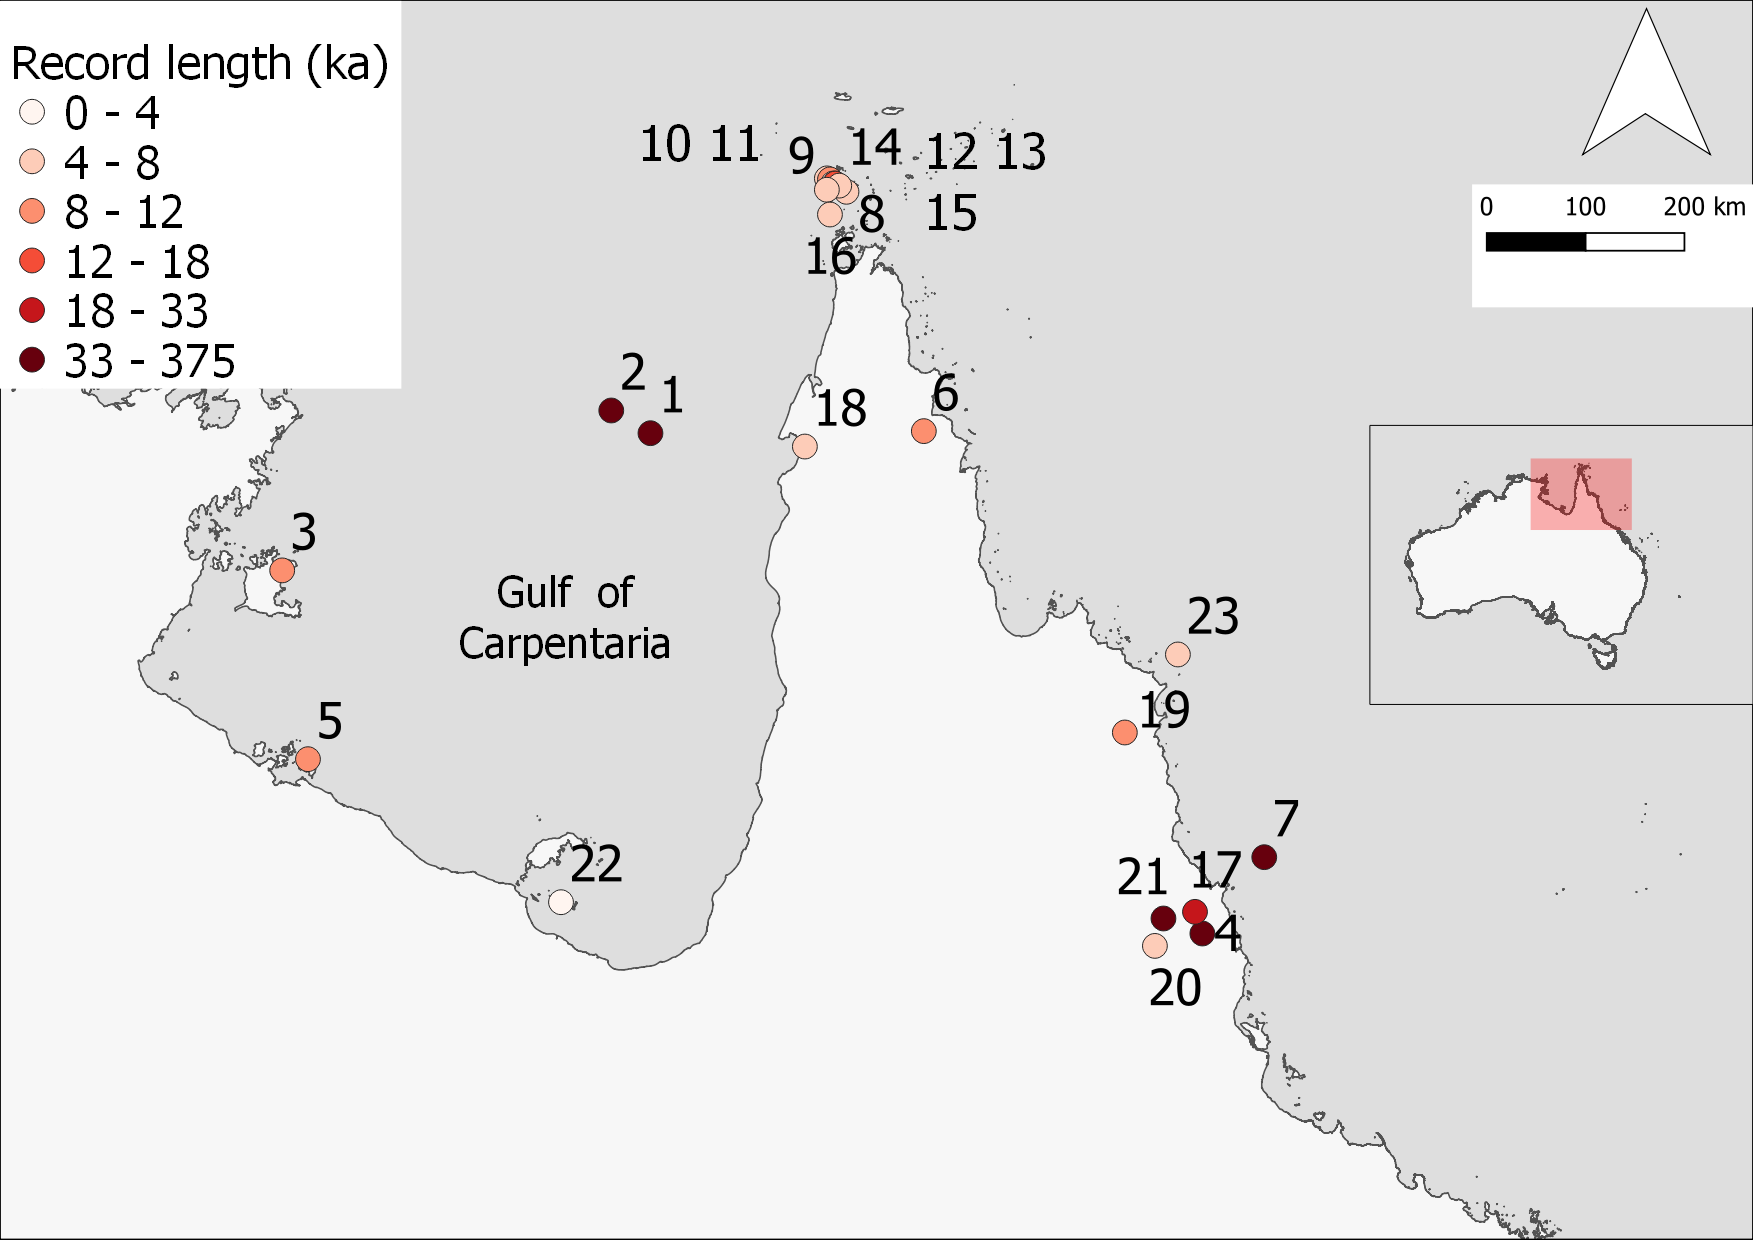
\includegraphics[width=1\linewidth]{C:/Users/Maria Jose Rivera/Documents/PhD/Figs/Background/cleaned_climate_2} 

}

\caption{Location of sites mentioned in the text (refer to Table \ref{tab:tb-sites} for details)}\label{fig:fig-climate}
\end{figure}



\begin{landscape}
\begin{longtable}[t]{rlrrlr>{\raggedright\arraybackslash}p{5cm}}
\caption{\label{tab:tb-sites}Latitude, longitude and length of the past environmental records discussed in the text}\\
\toprule
Number & Site & Latitude & Longitude & Type & Length (ka) & References\\
\midrule
\endfirsthead
\caption[]{\label{tab:tb-sites}Latitude, longitude and length of the past environmental records discussed in the text \textit{(continued)}}\\
\toprule
Number & Site & Latitude & Longitude & Type & Length (ka) & References\\
\midrule
\endhead
\
\endfoot
\bottomrule
\endlastfoot
1 & Lake Carpentaria GC2 & -12.52000 & 140.3500 & lacustrine & 36.00 & Torgersen et al., 1985, 1988\\
2 & Lake Carpentaria MD32 & -12.30000 & 139.9700 & lacustrine & 130.00 & Chivas et al., 2001; Reeves et al., 2008; Devriendt, 2011\\
3 & Four Mile Billabong, NT & -13.85000 & 136.7800 & swamp & 10.00 & Shulmeister and Lees, 1995\\
4 & Lynch's Crater, QLD & -17.37000 & 145.7000 & lacustrine & 234.75 & Kershaw, 1981; Turney et al., 2006; Kershaw et al., 2007\\
5 & Lake Walala, NT & -15.68000 & 137.0300 & swamp & 10.00 & Prebble et al., 2005\\
\addlinespace
6 & Three Quarter Mile Lake, QLD & -12.50000 & 143.0000 & lacustrine & 8.30 & Luly et al., 2006\\
7 & ODP820 & -16.63000 & 146.3000 & marine & 250.00 & Moss and Kershaw, 2000; 2007\\
8 & Mua, Torres Strait & -10.18000 & 142.2500 & swamp & 6.00 & Rowe, 2007\\
9 & Argan Swamp & -10.05000 & 142.0600 & coastal & 5.52 & Rowe, 2007\\
10 & Badu 15 & -10.06000 & 142.0900 & terrestrial & 9.00 & Rowe, 2007\\
\addlinespace
11 & Bar20 & -10.10000 & 142.1200 & coastal & 2.83 & Rowe, 2007\\
12 & Boigu Gawat Core 1 & -10.10000 & 142.1400 & coastal & 4.57 & Rowe, 2007; Rowe, 2015\\
13 & Boigu Gawat Core 2 & -10.10000 & 142.1400 & coastal & 13.82 & Rowe, 2007; Rowe, 2015\\
14 & Tiam Point & -10.12000 & 142.1800 & coastal & 7.70 & Rowe, 2007\\
15 & Zurath Islet & -10.16000 & 142.0600 & coastal & 6.50 & Rowe, 2007\\
\addlinespace
16 & Waruid & -10.40000 & 142.0900 & coastal & 6.00 & Rowe, 2007\\
17 & Lake Euramoo & -17.15990 & 145.6286 & lacustrine & 23.48 & Haberle, 2005\\
18 & Big Willum & -12.64929 & 141.8470 & lacustrine & 8.00 & Stevenson 2015\\
19 & Isabella Swamp & -15.42127 & 144.9486 & swamp & 9.20 & Stephens and Head 1995\\
20 & Witherspoon Swamp & -17.49000 & 145.2400 & swamp & 7.90 & Moss 2012\\
\addlinespace
21 & Bromfield Swamp & -17.22440 & 145.3227 & swamp & 37.00 & Burrows 2014; Burrows 2016\\
22 & Bentinck Island & -17.06660 & 139.4830 & coastal & 2.40 & Mackenzie et. al, 2017; Mackenzie et al., 2020\\
23 & Lizard Island & -14.66500 & 145.4630 & coastal & 8.00 & Proske and Haberle, 2012\\*
\end{longtable}
\end{landscape}



\hypertarget{LGM}{%
\subsubsection{Glacial (30 ka - 21 ka) and LGM (21 ka - 18 ka)}\label{LGM}}

The longest palaeoecological records from northern Australia come from Lake Carpentaria, and several studies have defined the extent and lake level fluctuations during the late Quaternary in this region \citep{jonesLateQuaternaryEvolution1988, mccullochStrontiumIsotopeVariations1989a, reevesPalaeoenvironmentalChangeGulf2007, reevesSedimentaryRecordPalaeoenvironments2008, torgersenLateQuaternaryHydrological1985a, devriendtLateQuaternaryEnvironment2011}. \citet{torgersenLateQuaternaryHydrological1985a} estimated the regional evaporation to precipitation ratio to have remained twice the modern ratio between 41 ka to 12 ka, suggesting drier conditions. Additionally, irregular patterns of precipitation during the LGM are suggested by the highly variable Mg/Ca, Na/Ca, Sr/Ca, and \(\delta\)\textsuperscript{18}O.

Additional evidence of aridity in northern Australia comes from analysis of aeolian dust activity \citep{dedeckkerLatePleistoceneRecord1991, dedeckkerLateQuaternaryCyclic2001} in the Gulf of Carpentaria. The most pronounced arid period peaks around 21.5 ka, corresponding to the start of the period of lowest global sea level and glacial advance. Other peaks were found at \textasciitilde{} 25.5 ka, \textasciitilde{} 29.5 ka, 24 ka, and 19.3 ka \citep{dedeckkerLateQuaternaryCyclic2001}. Furthermore, evidence of fluvial activity in the north of Australia generally supports drier conditions through the LGM \citep{nansonComparativeUraniumThoriumThermoluminescence1991, nansonQuaternaryStratigraphyGeochronology1993}.

There are no terrestrial records of climate, vegetation, and fire in Cape York between 30 ka - 18 ka. All of the available records are from south Cape York in the humid, not seasonal, tropics on the Atherton Tablelands. In this area, three sites have been extensively studied: Lynch's crater \citep{kershawCompletePollenRecord2007, turneyGeochemicalChangesRecorded2006a, turneyMillennialOrbitalVariations2004a}, Lake Euramoo \citep{haberle23000yrPollen2005}, and Bromfield swamp \citep{burrowsNewLateQuaternary2016a}. The available lines of evidence suggest the Glacial and LGM periods to be drier and cooler than today in this sector. Before the LGM, palynological analyses report dry, open woodlands on the Atherton Tablelands, Lynch's Crater and Lake Euramoo \citep{turneyMillennialOrbitalVariations2004a, kershawPleistoceneVegetationHumid1994}. Vegetation records from Lynch's Crater, Lake Euramoo \citep{haberle23000yrPollen2005} and ODP 820 \citep{mossLateQuaternaryMarine2007} suggest the dominance of sclerophyll woodland (i.e.~Casuarinaceae and Myrtaceae). Except for Lynch's Crater, other records from the region indicate increased presence of grasses during the LGM \citep{petherickClimaticEnvironmentalVariability2011}. Further evidence of elevated values of Poaceae during the LGM is found in the pollen record from nearby marine core ODP820 \citep{mossLateQuaternaryMarine2007}. \citet{burrowsNewLateQuaternary2016a} suggested marked changes in effective precipitation (towards drier conditions) at 32.7 ka, 30.1 ka, 24.7 ka, and 21.9 ka in Bromfield Swamp.

In the broader tropical Australasian region, most studies agree on evidence of drier, cooler conditions between \textasciitilde{} 33 ka and 18 ka across the area \citep{dennistonNorthAtlanticForcing2013, dinezioEffectSeaLevel2013a, reevesPalaeoenvironmentalChangeTropical2013}, with a lesser number reporting the existence of wetter events, some of them episodic \citep{nott30000Year1996, mullerPossibleEvidenceWet2008a, burrowsNewLateQuaternary2016a, dennistonDecouplingMonsoonActivity2017}. For instance, extreme flood events just before 23 ka were detected by \citet{nott30000Year1996} and \citet{nottWaterfallsFloodsClimate1999}, although the timing of these events should be taken with caution as dates could be overestimated \citep{mayRefiningLateQuaternary2015}. \citet{mullerPossibleEvidenceWet2008a} found evidence of wet conditions during Heinrich events at 30 ka -- 29 ka and 24 ka -- 23 ka in Lynch's Crater. Changes in monsoon strength during the LGM have been proposed by several studies \citep{jiangConceptGlobalMonsoon2015, dennistonDecouplingMonsoonActivity2017, yanUnderstandingAustralianMonsoon2018}. For example, \citet{yanUnderstandingAustralianMonsoon2018} found that while the annual mean precipitation over the Australian monsoon region decreased, the annual range was enhanced.

Except for Lake Carpentaria, all studies from the region have fire records, most of them younger than \textasciitilde{} 12 ka. Both Lynch's Crater and ODP 820 have records for the LGM and the Glacial, with high charcoal values during the LGM \citep{kershawPleistoceneVegetationHumid1994, mossLateQuaternaryMarine2007, kershawCompletePollenRecord2007} or increased availability of biomass (e.g.~sclerophyll woodland) for burning \citep{kershawPleistoceneVegetationHumid1994}.

\hypertarget{deglacial-18-ka---12-ka}{%
\subsubsection{Deglacial (18 ka - 12 ka)}\label{deglacial-18-ka---12-ka}}

The increase in lake level at Lake Carpentaria during the Deglacial suggests wetter conditions in the region, possibly associated with the reactivation of the monsoon. While wetter conditions are reported in Lake Euramoo related to the growth of \emph{Eucalyptus} woodland, Lynch's Crater and the ODP 820 records show evidence of dry conditions based on vegetation \citep{kershawQuantitativePalaeoclimaticEstimates1988, mossLateQuaternaryMarine2007, turneyMillennialOrbitalVariations2004a, kershawCompletePollenRecord2007}. Likewise, in Broomsfield swamp decreases in effective precipitation at 13.9 ka -- 13.4 ka and 11.9 ka were identified \citep{burrowsNewLateQuaternary2016a}.

Fire records in the dry tropics report negligible or low burning activity during this period \citep{roweHoloceneSavannaDynamics2019, fieldLateQuaternaryRecord2017}, except for Lake Euramoo, where fire was much more prominent in the landscape starting at 16.8 ka.

\hypertarget{holocene-12-ka---present}{%
\subsubsection{Holocene (12 ka - Present)}\label{holocene-12-ka---present}}

\begin{itemize}
\tightlist
\item
  Early Holocene (12 ka - 8 ka)
\end{itemize}

Warmer and wetter conditions have been proposed to be dominant during the early Holocene in the northern Australian tropics. Records from the west of the Gulf of Carpentaria (Four Mile Billabong and Walala) point to effective precipitation rises from \textasciitilde{} 10 ka to 5 ka. The very few studies from the savannas of Cape York are limited to those derived from lake sediment cores with records beginning at the middle Holocene. These studies include Big and Little Willum \citep{proskeHoloceneDiatomRecords2017a, stevensonPalaeoenvironmentalHistoryBig2015} and Three-Quarter Mile Lake \citep{lulyHolocenePalaeoenvironmentsChange2006}, and propose an increase in effective precipitation \textasciitilde{} 7.9 ka, consistent with studies from the Atherton Tablelands and the Kimberley \citep{shulmeisterHolocenePollenRecord1992, haberle23000yrPollen2005, dennistonStalagmiteRecordHolocene2013, roweHoloceneSavannaDynamics2019}. In Big Willum, as open water developed, from \textasciitilde{} 7 ka -- 5 ka, grass and sedge representation declined as the swampy basin bottom became fully submerged. Several coastal sites in the area (Western Torres Strait, Lizard Island) record widespread mangrove forest development led by the early Holocene sea level rise \citep{rowePalynologicalInvestigationHolocene2007, proskeIslandEcosystemBiodiversity2012}. Changes in vegetation suggest increased rainfall in Lake Euramoo. \citet{haberle23000yrPollen2005} found the maximum rate of increase in rainforest between 9.6 ka and 8.7 ka. These changes are most likely to represent the local establishment of closed canopy rainforest under the influence of increasing precipitation at Lake Euramoo.

\begin{itemize}
\tightlist
\item
  Mid and Late Holocene (8 ka - Present)
\end{itemize}

The middle Holocene has also been identified as a period of increased precipitation in the northeastern Australia's humid tropics and Western Torres Strait. In Broomfield Swamp, geochemical evidence derived from elemental counts (ITRAX) (rise in Ti and Ge) suggests a wetter period (8.5 ka - 5.9 ka) compared to the periods before and after \citep{burrowsNewLateQuaternary2016a}. Another phase of increased precipitation for Lake Euramoo is suggested around 7.3 ka to 6.3 ka, when rainforest achieved its maximum extent across the Atherton Tablelands. \citet{shulmeisterAustralasianEvidenceMidholocene1999} places the mid-Holocene precipitation maximum between 5 ka - 3.7 ka for the Northern Territory and north Queensland. In the Torres Strait, the prominence of island rainforest elements during the early-mid Holocene likely reflects the timing and influence of higher rainfall and humid climate. Additional evidence of a wetter phase is present at 6 ka in Lizard Island, where a possible cyclone event was documented \citep{proskeIslandEcosystemBiodiversity2012}. Extensive stable mangrove communities dominated coastal Torres Strait, starting at 6 ka and 3 ka \citep{rowePalynologicalInvestigationHolocene2007}. Overall, pollen from northern Australia also reflects woodland expansion at this time, and modern vegetation established \citep{proskeHoloceneRecordCoastal2014}. Whiterspoon swamp also shows a wetter phase during the mid-Holocene, with an increase in sedges and sclerophyll taxa \citep{mossHoloceneEnvironmentsSclerophyll2012a}.

Quantitative estimates derived from offshore pollen records also indicate peak precipitation between 7 ka and 6 ka \citep{vanderkaars100000yearRecord2006}. These changes are associated with the flooding of the continental shelf and the `big swamp phase', as sea levels increase during the deglaciation and early Holocene \citep{woodroffeDevelopmentWidespreadMangrove1985}.

Two increases in charcoal accumulation were identified at 8 ka in Lake Euramoo \citep{haberle23000yrPollen2005}, while in Big Willum a peak was identified at 7.2 ka \citep{stevensonPalaeoenvironmentalHistoryBig2015}. Vanderlin Island in the Gulf of Carpentaria shows an increase around 6 ka. In summary, these peaks suggest increased burning during the middle Holocene in the area.

In northern Australia, the late Holocene is associated with climatic variability, peat/wetland establishment and localised episodic aridity. For example, the available records from Lake Euramoo and Lynch's Crater agree that this period was characterised by increased seasonality \citep{haberle23000yrPollen2005, reevesPalaeoenvironmentalChangeTropical2013}. Similarly, \citet{headPalaeoecologyArchaeologyEast1992} identify ``increasing climatic variability'' in the last 3000 years from dune instability in the East Kimberley. Evidence and derived discussions from several sites across northern Australia from \citet{leesGeomorphologicalEvidenceLate1992a}, \citet{shulmeisterAustralasianEvidenceMidholocene1999}, and \citet{gaganPostglacialEvolutionIndoPacific2004}, including the western Torres-Strait \citep{rowePalynologicalInvestigationHolocene2007} point to conditions during the mid-to-late Holocene as much drier than the previous early-to-mid Holocene phase. \citet{haberle23000yrPollen2005} identifies drier conditions and increased rainfall seasonality after \textasciitilde{} 4 ka. \citet{stevensonPalaeoenvironmentalHistoryBig2015} note the end of a ``warm and wet period'' at \textasciitilde{} 5 ka at Big Willum Swamp and identify the period between 1 ka - 0.4 ka as the period of ``greatest variability'' at the site. Similarly, in Witherspoon swamp, \citet{mossEnvironmentalContextLate2015} identified a period of dry conditions starting at 2 ka.

\citet{burrowsNewLateQuaternary2016a} identified a dry event in the Bromfield Swamp and Quincan Crater records at 4.1 ka as a possible indicator of ``substantial climate change''. \citet{mackenzieGeochemicalInvestigationSouth2017} describe variable conditions over the last 1.25 ka in the South Wellesley Islands, including storm events, wet conditions at one site around 0.750 ka and a drying trend beginning in the last 150-50 years across three swamps.

The Late Holocene was also a period of wetland and peat establishment reported at several sites \citep{roweLateHoloceneSwamp2015, stevensonPalaeoenvironmentalHistoryBig2015, lulyHolocenePalaeoenvironmentsChange2006}. In the Torres Strait Islands, freshwater swamps developed by 2.6 ka with palynological records dominated by \emph{Melaleuca} and the herbaceous swamp taxa \emph{Leptocarpus} and Cyperaceae \citep{roweLateHoloceneSwamp2015}. Records at Boigu Gawat 1 and Boigu Gawat 2 in Torres Strait, suggest that wetlands became more productive, organic material increased and coastal influence was reduced \citep{rowePalynologicalInvestigationHolocene2007, roweLateHoloceneSwamp2015}. Records in the Gulf of Carpentaria show expansion and development in the late-Holocene. Walala swamp in Vanderlin Island was fully developed by 4.5 ka with organic sediments increasing in the last 2 ka \citep{prebbleHolocenePollenDiatom2005}. Four Mile Billabong also expanded in the last 1 ka. At Big Willum swamp increased precipitation is maintained between 2.2 ka and 1.3 ka \citep{proskeHoloceneDiatomRecords2017a}.

Locations such as the Torres-Strait \citep{roweLateHoloceneSwamp2015} show an increase in charcoal accumulation (and therefore, fire) during the last millennium before the present. Big Willum in Western Cape York shows peaks after 2 ka. Variable patterns of burning have been identified during the Late Holocene \citep{rowePalynologicalInvestigationHolocene2007, roweLateHoloceneSwamp2015, fieldCoherentPatternsEnvironmental2018, haberle23000yrPollen2005}. Some studies have argued that this pattern in the later Holocene reflects an increase in climate variability associated with more active ENSO cyclicity \citep{mooneyLateQuaternaryFire2011, kershawCompletePollenRecord2007}.

\hypertarget{palaeogeo}{%
\subsection{Palaeogeography of Cape York Peninsula (33 ka - Present)}\label{palaeogeo}}

This section presents the available information on changes on palaeogeography, specifically sea level and dune formation in northern Australia and the broader region. Cape York Peninsula underwent major changes in geography during the last 33 ka, especially related to changes in sea level. By compiling a range of Late Quaternary sea-level indicator data, \citet{brookePalaeoshorelinesAustralianContinental2017} and \citet{lambeckSeaLevelGlobal2014} found an abrupt decrease in sea level \textasciitilde{} 30 ka (from - 83 m to - 126 m) in the Australian/South Pacific region (Figure \ref{fig:fig-sea2}, Figure \ref{fig:fig-sea} and Table \ref{tab:gc}). In Lake Carpentaria, during MIS 3 (57 ka- 29 ka), fully lacustrine conditions are confirmed by the ostracod Ba/Ca ratios, and the lake level corresponding to the - 60 m bathymetric contour, including increased intensity of fluvial sediment transport occurred during the MIS 3 and MIS 1 \citep{reevesSedimentaryRecordPalaeoenvironments2008}.

Additional records from Lake Carpentaria indicate that lake levels dropped during the LGM (from the 59 m bathymetric contour during mid-MIS 3 to the 63 m bathymetric contour during the LGM). Episodes of sand deposition (aeolian or fluvial origin) at 26 ka, 24 ka and 21.5 ka at Lake Carpentaria are interpreted as arid events \citep{dedeckkerLateQuaternaryCyclic2001} that closely match periods of elevated monsoon rainfall in the Ball Gown Cave record (northwestern Australia) \citep{dennistonNorthAtlanticForcing2013}. During the LGM, large fluctuations of the lake level at the seasonal and interannual time scale are inferred from the \(\delta\)\textsuperscript{18}O values and trace-element ratios of ostracod shells \citep{devriendtLateQuaternaryEnvironment2011}. Fluvial activity continued through this period to maintain the lake permanently in the deeper regions of the basin. The sedimentary record indicates a temporary contraction of the lake to around the − 63 m contour (23--19 ka), during which the sea was at its lowest level (approximately − 125 m) \citep{brookePalaeoshorelinesAustralianContinental2017, yokoyamaShorelineReconstructionAustralia2001}.

Lowered glacial sea level exposed the Sahul shelf, the continental shelf extending over from the northern coast of Australia to the island of New Guinea, south of the Gulf of Carpentaria and the Timor Sea. Its exposure could have sizable impact on IPWP climate given their central location between areas of deep convection of the IPWP \citep{dinezioClimateResponseIndo2016} (Figure \ref{fig:fig-sea3}).

Low sea levels during the LGM also influenced dune formation and emplacement in tropical Australia (Figure \ref{fig:fig-geo}). Dune emplacements in Cape Arnhem \citep{leesThermoluminescenceDatingDune1995}, Cape Flattery and Shelburne Bay between 24 and 18 ka appear to represent a period of widespread dune activity associated with the LGM. Dune formation occurred at glacial low sea levels when wide areas of continental shelf became exposed to wind action \citep{leesReconnaissanceThermoluminescenceDating1990, leesGeomorphologicalEvidenceLate1992a, leesTimingFormationCoastal2006} (Figure \ref{fig:fig-sea}).

Lagoons also record aeolian and dune activity. For example, in Native Companion Lagoon (NCL), in North Stradbroke Island (southeast Queensland), the significant local sand and dust content of the NCL record for this period indicate that the dunes surrounding NCL were active, most likely in response to a reduced cover of vegetation. The LGM is shown as the period of maximum aeolian sedimentation, as a result of decreased precipitation. Loss of vegetation cover and subsequent destabilization of dunes would account for the increased deposition of local North Stradbroke Island sediments in Native Companion Lagoon at this time \citep{petherickReconstructingTransportPathways2009, mcgowanAeolianSedimentationClimate2008}.

In a regional context, several studies have highlighted the impact of changing sea levels on the hydroclimate. For example, \citet{dinezioEffectSeaLevel2013a} highlight the importance of continental shelf exposure during low sea levels on IPWP hydrology during the LGM, when comparing the results from several studies in the region. The study by \citet{dinezioEffectSeaLevel2013a} also suggests that sea level is a first-order driver of tropical hydroclimate on glacial--interglacial timescales, and that the exposure of the Sunda Shelf best explain the pattern of hydroclimatic change inferred from the proxies. Dry conditions may have been maintained until flooding of the Sunda--Sahul shelf, at the end of the deglaciation, according to several studies \citep[e.g.~][]{dedeckkerStatusIndoPacificWarm2003, dinezioEffectSeaLevel2013a}.

\begin{figure}

{\centering 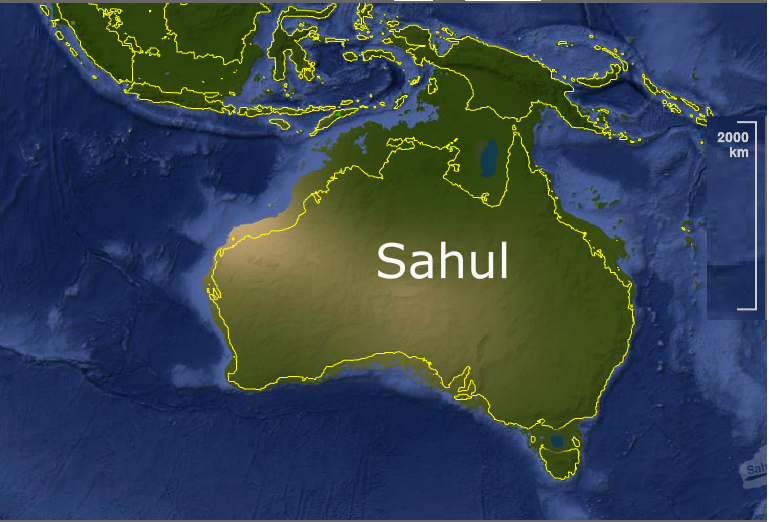
\includegraphics[width=0.8\linewidth]{C:/Users/Maria Jose Rivera/Documents/PhD/other/Background/sahul_2} 

}

\caption{Sahul \textasciitilde{} 20 ka. Yellow line denotes modern coastline. Source: \url{http://sahultime.monash.edu.au/}}\label{fig:fig-sea3}
\end{figure}



\begin{figure}

{\centering 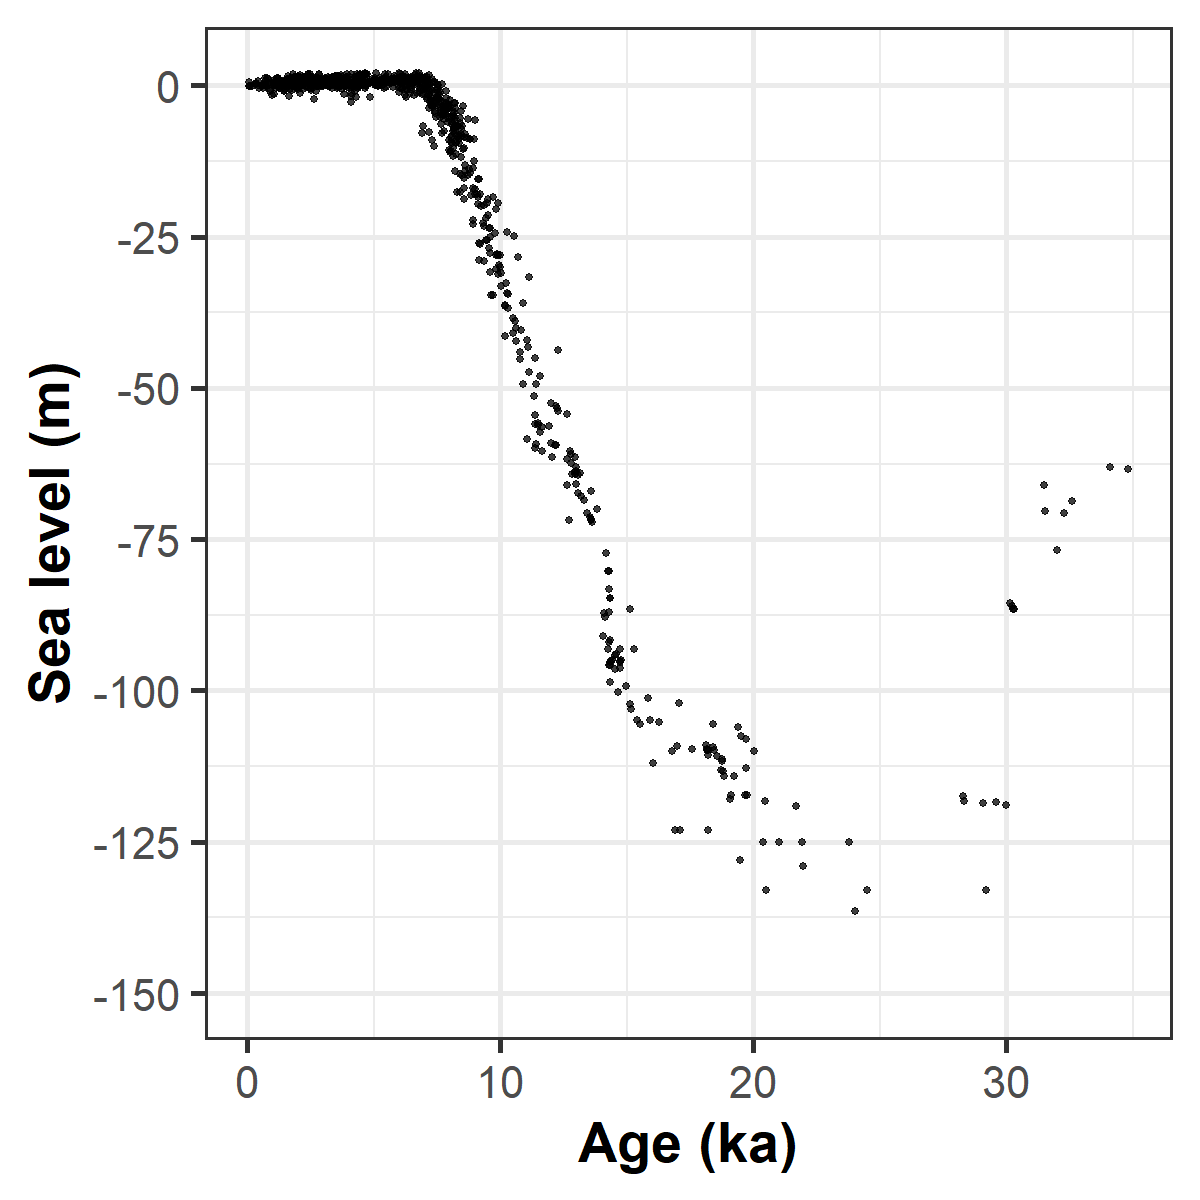
\includegraphics[width=0.8\linewidth]{C:/Users/Maria Jose Rivera/Documents/PhD/Figs/Background/sea_level_3} 

}

\caption{Changes in sea level according to \citet{lambeckSeaLevelGlobal2014}}\label{fig:fig-sea2}
\end{figure}



At Lake Carpentaria, beginning at 18 ka there is evidence of increased run-off and weathering. Increasing contributions from southern rivers and decreased salinity during 18 ka - 15 ka are interpreted as evidence of the reactivation of the monsoon. Sedimentological evidence suggests a significant increase in lake level and extent after 18 ka \citep{reevesSedimentaryRecordPalaeoenvironments2008}. This is confirmed by freshening of the lake and a considerable decrease in the lake water \(\delta\)\textsuperscript{18}O variability after 18 ka \citep{reevesSedimentaryRecordPalaeoenvironments2008}. The maximum lake level (\textgreater{} 3 m average depth) and extent (\textgreater{} 100,000 km\textsuperscript{2}), as well as the lowest salinity, are recorded between 14 ka and 12 ka, suggesting the monsoon reached northeastern Australia around this time \citep{reevesSedimentaryRecordPalaeoenvironments2008}. A shell-rich layer (19.0 ka -- 17.1 ka) indicates a highly productive environment, associated with an influx of fresh water and increased precipitation. These changes are reflected in the sea level curve built by \citet{brookePalaeoshorelinesAustralianContinental2017}.

In the western equatorial Pacific (Sulawesi, Indonesia), dry conditions during the late glacial were terminated as a result of rising sea levels and the inundation of shallow continental shelves in the region, after the onset of deglaciation \citep{dinezioEffectSeaLevel2013a, griffithsAbruptIncreaseEast2013}. Significant changes in speleothem \(\delta\)\textsuperscript{18}O also coincide with the rapid flooding of the Sahul (\textasciitilde{} 12 ka -- 11 ka) and Sunda (\textasciitilde{} 8.5 ka) shelves \citep{krauseSpatiotemporalEvolutionAustralasian2019}. The corresponding changes in speleothem \(\delta\)\textsuperscript{18}O at Sulawesi likely represent a combination of the reorganisation of local water masses, changes in source moisture pathways and intensification of the Walker circulation caused by enhanced convection over newly formed seas in the western equatorial Pacific region \citep{griffithsIncreasingAustralianIndonesian2009, dinezioEffectSeaLevel2013a, krauseSpatiotemporalEvolutionAustralasian2019}.

From \textasciitilde{} 12 ka important changes in sea level are recorded based on studies from Lake Carpentaria and the South Wellesley Archipelago \citep{slossHoloceneSealevelChange2018a}. From 12 ka, oceanic waters transgressed the Arafura Sill, and by 10.7 ka, the Lake Carpentaria region had become marine \citep{mccullochStrontiumIsotopeVariations1989a, chivasSealevelEnvironmentalChanges2001}. Full marine conditions attained in the Gulf of Carpentaria by 10.5 ka. \citet{slossHoloceneSealevelChange2018a} found that sea-level rose from −53 m (depth of the Arafura Sill) \citep{reevesSedimentaryRecordPalaeoenvironments2008, slossHoloceneSealevelChange2018a, harrisNewCoralReef2008} at ca. 11.7 ka to ca. --25 m by 9.8 ka \citep{slossHoloceneSealevelChange2018a} culminating in a mid-Holocene sea-level highstand (7.7 ka-- 4 ka) and a corresponding period of increased precipitation and temperature during the Holocene. Coastal flooding facilitated increased moisture and heat transfer/transport fueling monsoon activity. Data from Karumba, in the southern Gulf of Carpentaria, indicate that sea level was 2.5 m higher around 6.4 ka. Possibly, these conditions would increasily expose Sanamere Lagoon to moisture and wind from the sea more than ever before. After 2 ka, sea level fell to present level \citep{lewisPostglacialSealevelChanges2013a}.

Additional studies from stalagmites in southeast Indonesia \citep{griffithsIncreasingAustralianIndonesian2009} also support the idea that lowered sea level had a large effect on IPWP hydroclimate from the LGM to 9.5 ka, when the Sunda Shelf was nearly flooded. Moreover, the early Holocene intensification of monsoon precipitation was driven by sea-level rise, which increased the supply of moisture to the Indonesian archipelago. Monsoon precipitation intensified even more rapidly from 11 ka to 7 ka, when the Indonesian continental shelf was flooded by global sea-level rise.

\begin{figure}

{\centering 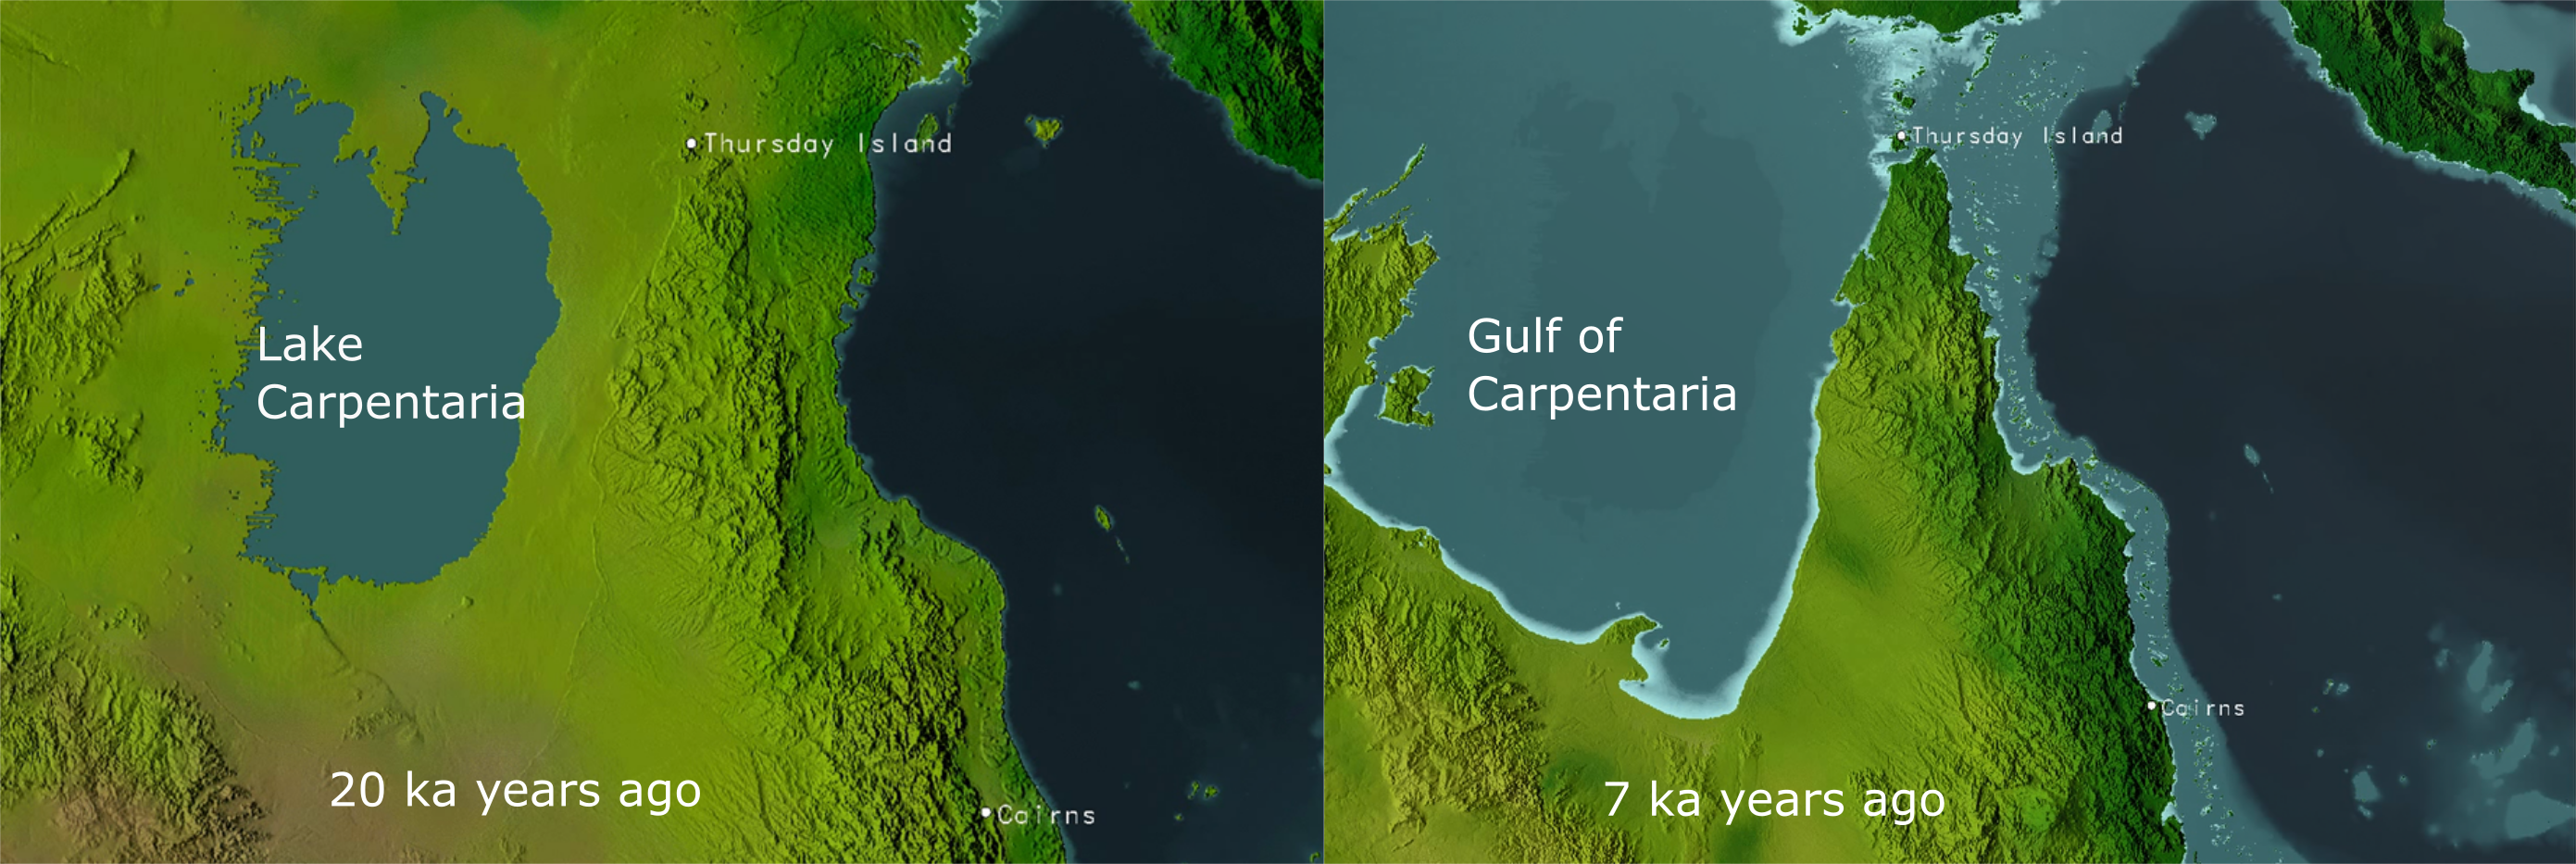
\includegraphics[width=1\linewidth,height=1\textheight]{C:/Users/Maria Jose Rivera/Documents/PhD/Figs/Background/sea_level_thesis_2} 

}

\caption{Changes in sea level in the Gulf of Carpentaria}\label{fig:fig-sea}
\end{figure}



\begin{table}

\caption{\label{tab:gc}Main sea level changes in the Gulf of Carpentaria}
\centering
\begin{tabular}[t]{lll}
\toprule
Date (ka) & Event & Reference\\
\midrule
57 - 23 & Low sea levels & Reeves, 2008\\
23 - 18 & Lowest sea levels & Devriendt,2011\\
18 - 14 & Increase in sea level & Devriendt 2011\\
14.1 & Sea level rise rapidly & Brooke, 2017\\
11.7 & Breaching of the Arafura Sill & Sloss 2018\\
\addlinespace
10.5 & Full marine conditions & Sloss 2018\\
7.7- 4 & High stand & Sloss 2018\\
4- Present & Present day sea level & Sloss 2018\\
\bottomrule
\end{tabular}
\end{table}



A drying trend is noted in several of the records during the mid Holocene (Ball Gown Cave, Black Springs) and speleothems of Flores, coincident with increased precipitation in Borneo. A contraction of the IPWP is also recorded in the corals of this region \citep{reevesPalaeoenvironmentalChangeTropical2013}.

The re-establishment of vegetation caused by rising sea levels during the mid Holocene also contributed to dune stabilisation. The impact of sea level regression during the late Holocene is also documented in Bentinck Island, where the mangrove community transitioned to woodland and wetland dominated vegetation over the last 850 years \citep{mackenzieLateHoloceneRecordCoastal2020}. These changes also determined the timing of wetland development on the site, transitioning from coastal environments to wetlands between 0.8 and 0.4 ka \citep{mackenzieGeochemicalInvestigationSouth2017}.

\begin{figure}

{\centering 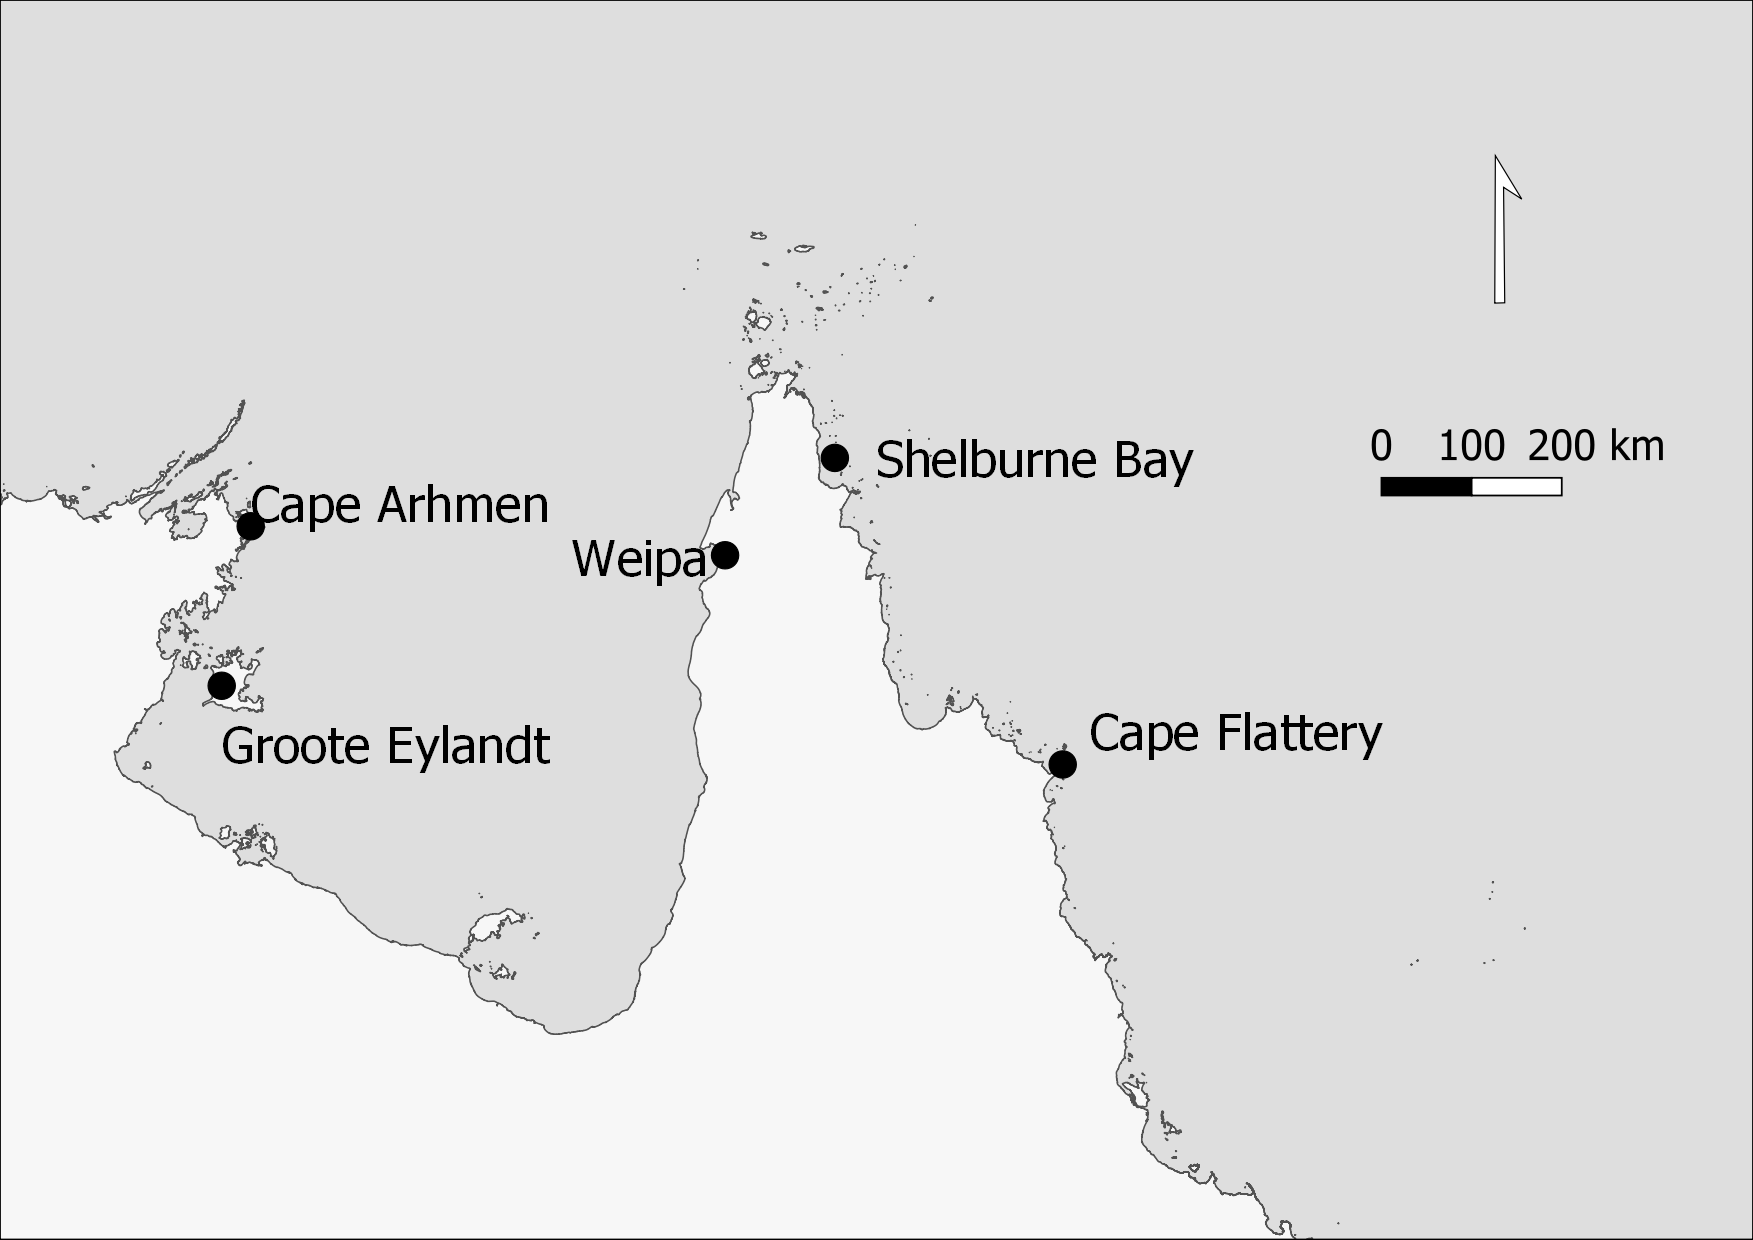
\includegraphics[width=1\linewidth,height=1\textheight]{C:/Users/Maria Jose Rivera/Documents/PhD/Figs/Background/paleo_geo} 

}

\caption{Sites with evidence of dune activity in Cape York Peninsula and surroundings}\label{fig:fig-geo}
\end{figure}



\hypertarget{background-to-the-methods-used-in-the-thesis}{%
\section{Background to the methods used in the thesis}\label{background-to-the-methods-used-in-the-thesis}}

The following sections develop the theoretical framework to interpret the results from chapters 3, 4, 5 and 6. Chapter 3 examines the sedimentology and stratigraphy of the Sanamere lake sediment core. Chapter 4 examines six carbon fractions in the sediment samples to determine which fraction and technique pre-treatment is most appropriate to obtain reliable radiocarbon dating results. Chapters 5 and 6 describe the palaeoenvironmental reconstruction for Sanamere Lagoon using multiple proxy records.

\hypertarget{geochronology-aim-i}{%
\subsection{Geochronology (Aim I)}\label{geochronology-aim-i}}

\hypertarget{hypy}{%
\subsubsection{Radiocarbon dating}\label{hypy}}

The ubiquitous presence of carbon in lacustrine environments makes radiocarbon dating one of the most commonly used and established techniques to date lake sediments. Carbon has three naturally occurring isotopes, two of which are stable (C-12 and C-13) and one (C-14) which is unstable or radioactive. The production of C-14 takes place as a result of several nuclear reactions of \textsuperscript{14}N with cosmic rays to form C-14 and a proton. Within hours, C-14 atoms undergo oxidation to form carbon dioxide (\textsuperscript{14}CO\textsubscript{2}). Once a \textsuperscript{14}C-tagged CO\textsubscript{2} molecule reaches the surface of the earth, it enters into the carbon cycle. About 85 \% of C-14 remains in ocean water and the rest stays in terrestrial environments, where plants fix it in their cellular structures by photosynthesis, while other organisms obtain it secondarily by ingestion. Metabolic processes maintain the C-14 content of living organisms in equilibrium with atmospheric C-14. These metabolic processes cease at the death of an animal or plant and the amount of C-14 will begin to decrease by decay at a rate determined by the C-14 half-life. The radiocarbon age of a given sample is based on measurement of residual C-14 content \citep{aitkenSciencebasedDatingArchaeology1990, woodRevolutionConventionPresent2015}.

Some of the challenges associated with working with radiocarbon dating include changes in the natural production rate of radiocarbon in the atmosphere and sample integrity. Regarding the first factor, the atmospheric production of radiocarbon has varied through time, and these changes cause systematic offsets between radiocarbon ages and calendrical ages. Calibration curves calculated by dating materials of precisely known age, such as tree rings have been used to overcome this discrepancy \citep{aitkenSciencebasedDatingArchaeology1990}. IntCal20, the most updated calibration curve includes a wealth of new data and was extended to 55,000 cal BP \citep{reimerIntCal20NorthernHemisphere2020}.

Regarding the second factor, the ability of a C-14 determination to accurately date an event depends on the integrity of the sample and the degree of association between the dated material and the event of interest. The integrity of the sample can be compromised by the incorporation of foreign carbonaceous materials into a sample matrix. For lake sediments, stratigraphic mixing, for example, by bioturbation is a common and serious problem, as it compromises the integrity of the sample. Bioturbation is one of the main causes of younger particles being reworked included in older deposits and viceversa. Erosion and floods can cause remobilized older carbon to be included in younger deposits. Samples that are in contact with groundwater could have absorbed inorganic carbonates that may alter the `true' date. The effect of contaminants can be mitigated if information about the age of the contaminant, and the percentage contribution of the contaminant is available, though this is rarely possible \citep{aitkenSciencebasedDatingArchaeology1990, woodRevolutionConventionPresent2015}.

\begin{itemize}
\tightlist
\item
  Selection of carbon fraction and pretreatment
\end{itemize}

Given the importance of the integrity of the sample to the reliability of radiocarbon dating, the selection of the carbon fraction to date and the pretreatment to apply is fundamentally important. There is general agreement about the suitability of some materials for dating, including very delicate materials, such as whole terrestrial leaves (which are unlikely to survive long periods of transport and reworking). There is more controversy around the general suitability of some macrofossils and charcoal, which have been reported to account for anomalous dates. Macrofossils can take up contamination from fungi \citep{wohlfarthPitfallsAMSRadiocarbondating1998} and have been shown to yield systematic differences between series of paired analyses on two types of macrofossils \citep{turneyImplicationsDatingWisconsinan2000}. Other materials, including bulk sediment and pollen, have been widely used, but previous studies have shown them to yield anomalous ages in at least some cases \citep{wangRadiocarbonDatingSoil1996}. Stable polycyclic aromatic carbon (SPAC) has been proposed as an alternative to the issues shown in other materials \citep{fieldUntanglingGeochronologicalComplexity2018, orrImprovedPretreatmentMethod2020}.

\emph{Hypy fraction}

Pyrogenic carbon (PyC) (hereafter Hypy fraction) with and aromatic ring size of \textgreater{} 7, is the solid carbonaceous residue remaining after hydrogen pyrolysis (hypy) and it is a demonstrably indigenous component of the original charcoal \citep{meredithAssessmentHydropyrolysisMethod2012}. As such, the hypy fraction is likely to produce a reliable radiocarbon date, as the processes remove labile carbon including contaminants (\textgreater{} 98 \%) \citep{orrImprovedPretreatmentMethod2020}. Although a relatively new technique, hypy has been successfully applied in a number of different studies \citep{birdEfficiencyCharcoalDecontamination2014, fieldCoherentPatternsEnvironmental2018}. Incomplete removal of modern contamination has been shown for charcoal formed at \textless{} 350 °C as a small fraction of the labile carbon component may also be pyrolysed during HyPy treatment \citep{birdEfficiencyCharcoalDecontamination2014}. During hypy, samples undergo pyrolysis aided by high hydrogen pressures in the presence of sulphided molybdenum catalyst \citep{ascoughHydropyrolysisNewTool2009, ascoughHydropyrolysisImplicationsRadiocarbon2010, wursterQuantifyingAbundanceStable2012}.

\emph{Bulk organics (bulk organic matter)}

When no macro-organic remains are visible in lake sediment matrices, dating bulk sediments is the one of the most commonly used options. The organic components of bulk sediments are divided in three main categories, according to their solubility in acid and base \citep{vanderplichtRadiocarbonDatingSoil2019, baylissRollingOutRevolution2009}.

\begin{itemize}
\tightlist
\item
  Humic acids: alkali soluble, acid insoluble and thought to derive from the decay of plant material that grew on the site as the sediment accumulated.
\item
  Humin: acid and alkali insoluble, thought to consist of the physical remains of the plant/algal material. Humins are generally considered to be the most stable C fraction within the sedimentary profile \citep{pessendaRadiocarbonDatingTotal2001}.
\item
  ``Total organic'' fraction: remains after the acid soluble fraction has been removed. ``Humic acid'' and ``humin'' fractions combined.
\end{itemize}

Given the multiple sources from which carbon could have derived \citep{bronkramseyRadiocarbonDatingRevolutions2008}, the contribution of contaminants increases considerably for any bulk organic matter fraction. Several studies have found this fraction to be consistently younger than other fractions \citep{wangRadiocarbonDatingSoil1996, pessendaRadiocarbonDatingTotal2001}.

\emph{Pollen concentrate}

Pollen concentrate is used as another alternative when macroscopic carbon fractions are not available. Several studies have found pollen concentrates to yield older \textsuperscript{14}C dates compared to other fractions \citep{neuliebPotentialPitfallsPollen2013, fletcherAMSRadiocarbonDating2017}, while others have found it to be younger \citep{mayEstablishingChronologicalFramework2018}, yielding significantly different chronologies compared to other fractions. In part this may be due to the greater mobility of pollen and pollen sized material in some environments \citep{clymoUpwashDownwashPollen1987} and therefore, the possibility of being reworked. In addition, the porous structure and high surface to volume ratio of the pollen grain walls make them prone to store exogenous carbon materials \citep{kilianProblematic14CAMSDates2002a}. These impurities can lead to unreliable dates \citep{fletcherAMSRadiocarbonDating2017}.

\emph{Cellulose}

Although cellulose is considered one of the fractions that yields reliable dates, the extraction of holocellulose is commonly complex and in some cases unreliable. For instance, during the early Holocene, differences of up to 1000 years are observed between lake sediment cellulose and terrestrial plant fossils. This disagreement is probably caused by the contribution of 14C-depleted cellulose synthesized by aquatic plants/algae in the lake \citep{kitagawaRadiocarbonConcentrationLake2007}.

Furthermore, the most commonly used procedures to extract cellulose are time-consuming and require excessive organic solvents \citep{wolfeProgressIsotopePaleohydrology2007}. Recently, \citet{gillespieNovelCellulosepreparationMethod2019} implemented a novel extraction protocol that includes the use of less toxic chemicals in quicker steps to overcome the disadvantages inherent in the previous procedures.

\emph{Macro/microcharcoal}

Macrocharcoal (\textgreater{} 250 \(\mu\)m) and microcharcoal (\textless{} 250 \(\mu\)m,\textgreater{} 63 \(\mu\)m) are very commonly dated when available, and considered to be inert. However, standard pretreatment can lead to unremoved contamination and samples can be destroyed after this procedure, with no remaining material to be dated \citep{birdIsotopesPyrogenicCarbon2012}. Additionally, \citet{birdCharcoal2007} showed that chemical modifications can occur on the surface of charcoal and that its porous nature makes it especially prone to absorb exogenous carbon and microbes. Iron carbonate (siderite) and oxides of different cations may also be formed during diagenesis. If this source of carbon is not removed, it can lead to anomalous dates \citep{birdCharcoal2007}.

Although they are usually not separated, some studies suggest that microcharcoal and macrocharcoal represent different sources, with microcharcoal coming from further way from the site deposition (as fine particles are more likely to be transported by wind or water over long distances before deposition in the location from which they are ultimately collected) compared to macrocharcoal, which is unlikely to move long distances. This difference could yield different radiocarbon dates for macro and microcharcoal from the same sample \citep{carcaillet2001comparison}.

\hypertarget{environmental-change-and-palaeohydrology-aims-ii-and-iii}{%
\subsection{Environmental change and palaeohydrology (Aims II and III)}\label{environmental-change-and-palaeohydrology-aims-ii-and-iii}}

Chapter 5 presents a multi-proxy record of geochemical (micro X-ray fluorescence {[}\(\mu\)XRF{]} scanning), carbon and nitrogen content and associated stable isotopes, physical (grain size) and biological (diatom) proxy data sets for Sanamere Lagoon. The Chapter aims to develop a record of hydroclimatic changes in an under-studied region of northeast Australia. Chapter 6 contributes to refining the vegetation and fire record using a phytolith, carbon isotope and pyrogenic carbon-based reconstruction of Sanamere Lagoon in northern Cape York, Australia. The following sections present the methodological foundation for these chapters.

\hypertarget{palaeohydrology}{%
\subsection{Palaeohydrology}\label{palaeohydrology}}

\begin{itemize}
\tightlist
\item
  Diatoms
\end{itemize}

Carbonates are one of the most commonly used materials in palaeohydrological studies, and they are used to infer the isotope composition of the lake water at its time of formation, and by inference the isotope composition of precipitation. Precipitation isotope ratios have been correlated with mean surface air temperature at mid-to high-latitudes, or with the amount of precipitation in tropical areas. However, in non-alkaline, dilute, open lakes, carbonates may be rare or absent. In lakes where carbonate is not preserved, silica bodies can be used as an alternative isotope proxy host to carbonates \citep{huBiogenicsilicaD18ORecord2003, lambComparisonPalaeoclimateSignals2005}. For example, diatoms are photosynthetic algae that secrete a shell composed of opaline silica (SiO\textsubscript{2}·nH\textsubscript{2}O) and are present in many lake sedimentary records. In very alkaline lakes (\textgreater{} pH 9) or lakes where silica is limited, diatoms are often preserved only in low concentration \citep{barkerExperimentalDissolutionDiatom1994}.

Diatom species inhabit specific environments based on their tolerance ranges and morphology \citep{battarbeeDiatoms2002}. For palaeoenvironmental purposes, classification systems use pH, habitat and salinity as determinant variables to understand changes in diatom abundance in the past. Habitat can be placed into two categories: benthic and planktonic species. Planktonic species live as free-floating cells in the plankton of ponds, lakes and oceans. Benthic species form attachments to surfaces and are further classified according to their attachment to the substratum. Epilithic species attach to rocks and geological surfaces, epipsammic species to sand grains, epizoic species to animals and epiphytic species are those that attach themselves to plants and other algae species. Finally, epipelic species are those that live on the benthos or sediment on the bottom of the aquatic environment while endopelic species live within sediment \citep{battarbeeDiatoms2002} (Table \ref{tab:tb-diat} and Table \ref{tab:tb-diat2}).

Diatoms are among the most common proxies that have been used for a long time in tropical areas to infer lake level, with the first studies pursued in Africa \citep{gasseLateQuaternaryLakelevel1978, gasseDiatomsReconstructingPalaeoenvironments1987}. Diatom composition and relative abundances potentially offer a more precise measure of palaeohydrological change than palynological data \citep{prebbleHolocenePollenDiatom2005, wolinDiatomsIndicatorsWaterlevel2010}. Other lake characteristics that are derived from these organisms include pH, sedimentary processes, changes in evaporation, salinity, turbidity and trophic status of a water body \citep{proskeHoloceneDiatomRecords2017a}. Diverse applications and research questions in arctic and subartic regions include peat water content, flood frequency, river discharge, effective moisture and ice cover \citep{moserPaleohydrologyInferredDiatoms2000}. The inclusion of oxygen stable isotope analysis on diatoms (\(\delta\)\textsuperscript{18}O\textsubscript{diatom}) has allowed the calculation of quantitative parameters including temperature and precipitation. \(\delta\)\textsuperscript{18}O\textsubscript{diatom} has been used as a proxy for climate and hydrological change in many studies across many geographical regions \citep{lengRecentAdvancesIsotopes2013, lengReviewOxygenIsotope2006}. The mineral-water isotope fractionation factor has been estimated previously from analyses of diatoms from freshwater (and marine) sediments. Several studies show that in lacustrine (and marine) systems no oxygen isotope vital effect exists in diatoms \citep{lengReviewOxygenIsotope2006}.

Diatoms have provided considerable information about the palaeohydrology and hydroclimate of many tropical regions, including Australia \citep{lulyHolocenePalaeoenvironmentsChange2006, prebbleHolocenePollenDiatom2005, proskeHoloceneDiatomRecords2017a, tibbyLateGlacialPresent2007}, with the majority of the studies pursued in the east portion of the continent. For example, autecological information from different species indicate changes in the water level of the lakes \citep{proskeHoloceneDiatomRecords2017a, tibbyLateGlacialPresent2007} or major shifts in local hydrology, e.g.~from a perennial swamp to open lake. Perennial lake conditions are identified by the overlap between planktonic/benthic and littoral/benthic diatom taxa \citep{prebbleHolocenePollenDiatom2005}.

The environmental inferences drawn from diatoms are based on the autecology of individual diatom species or the study of the interactions of each species with the living and nonliving factors of its environment. For example, inference models link diatom ecological tolerances with physico-chemical variables that can be used to and infer palaeoecological conditions \citep{battarbeeDiatoms2002}. On Cape York Peninsula, diatom composition is correlated with total alkalinity, bicarbonate concentration, pH, electrical conductivity (EC) and latitude \citep{negusSubtleVariabilityWater2019}. This correlation confrms the potential of using these organisms as palaeoclimate proxies in this area.

\begin{table}

\caption{\label{tab:tb-diat}Diatom classification according to salinity}
\centering
\begin{tabular}[t]{ll}
\toprule
Description & Salinity (\%)\\
\midrule
fresh & < 0.2\\
fresh brackish & < 0.9\\
brackish fresh & 0.8 - 1.8\\
brackish & 1.8 - 9.0\\
\bottomrule
\end{tabular}
\end{table}



\begin{table}

\caption{\label{tab:tb-diat2}Diatom classification according to pH}
\centering
\begin{tabular}[t]{ll}
\toprule
Classification & pH\\
\midrule
acidobiontic & optimal occurrence at pH < 5.5\\
acidophilous & mainly occurring at pH < 7\\
circumneutral & mainly occurring at pH-values about 7\\
alkaliphilous & mainly occurring at pH > 7\\
alkalbiontic & exclusively occurring at pH > 7\\
\addlinespace
indifferent & no apparent optimum\\
\bottomrule
\end{tabular}
\end{table}



\begin{itemize}
\tightlist
\item
  Sediment and isotope geochemistry
\end{itemize}

Titanium concentration and grain size analysis are commonly used to infer runoff and transportation of clastic materials into a lake \citep{vazquezHolocenePaleohydrologyEtzatlanMagdalena2017}. As with other proxies based on sediment physical properties, this depends on a clear understanding of climatic effects on sedimentology for a specific catchment \citep{douglasMethodsFutureDirections2016}. The presence of elements such as iron, titanium and aluminum in lake and marine sediments often indicate times of greater material transport under conditions of higher precipitation and consequent runoff. The drivers of bulk sediment elemental geochemistry vary widely, and often need to be determined for each catchment and sedimentary system.

The \(\delta\)\textsuperscript{13}C measurements of bulk sediments can be used to infer changes in the source of organic carbon in lake sediments. In some cases, such measures provide insights into vegetation change, and distinction between terrestrial and aquatic input, C\textsubscript{3} (trees and shrubs) and C\textsubscript{4} plants (tropical grasses), which can be related to climate \citep{maysStableCarbonIsotopes2017}.

\begin{itemize}
\tightlist
\item
  Grain size
\end{itemize}

Variability in clastic grain size can indicate changing lake levels, and the amount and energy of runoff into a sedimentary basin. Likewise, grain size analysis can be an indicator of the amount and intensity of flood events \citep{conroyHoloceneChangesEastern2008}. Some studies suggest that increased precipitation in closed-basin lake catchments transport larger grains from the catchment. Therefore, grain size in the sediment is seen as a function of the intensity and/or amount of rainfall \citep{chenEnvironmentalRecordsLacustrine2004}. Grain size measurements inform on the sources of detrital material and may help determine possible depositional processes (fluvial or aeolian) prevailing through different periods \citep{burrowsNewLateQuaternary2016a}. In Lake Barrine, in northeast Australia, grain size analysis, along with other proxies, was taken to indicate fluctuations in water level \citep{walkerHoloceneSedimentsLake2007}.

\hypertarget{fire-1}{%
\subsection{Fire}\label{fire-1}}

Optical charcoal analysis is commonly used as a proxy for fire activity in the past. Although the use of hypy fractions as a tracer of past fire activity is in its infancy, the study by Bird et al.~(2019) found that hypy fractions are able to reproduce similar fire activity signals when compared to charcoal counting records in northern Australia, with the advantage of removing the time-consuming particle counting step. Furthermore, the measurement of the carbon isotope composition of the pyrogenic carbon provides information on the proportions of C\textsubscript{3} and C\textsubscript{4} (grass) vegetation being burnt. In the study by Bird et al.~(2019), the recurrence of fire regimes (linked to changes in vegetation and climate) were derived using pyrogenic carbon abundance measured by hydrogen pyrolysis \citep{wursterQuantifyingAbundanceStable2012} (section \ref{hypy}). However, the results from optical charcoal analysis and the Hypy fraction are not directly comparable as the proportion of pyrogenic carbon (Hypy fraction) to charcoal increases with increasing fire intensity (therefore representing higher intensity fires compared to the macroscopic and microscopic charcoal particles) \citep{birdIsotopesPyrogenicCarbon2012}.

The study of fire regime in the past mostly relies on the measurement of charcoal abundance in sediments \citep{higueraPeakDetectionSediment2010}, and particle counting, either manually \citep{aliComparingFirehistoryInterpretations2009} or using computer-assisted tools \citep{conederaReconstructingFireRegimes2009a}. As an alternative, the abundance of pyrogenic carbon (measured by an incandescence‐based method) has been found to work as a moderate tracer of historical fire activity \citep{chellmanIncandescencebasedSingleparticleMethod2018}.

\hypertarget{backveg}{%
\subsection{Vegetation}\label{backveg}}

\begin{itemize}
\tightlist
\item
  Carbon isotopes \(\delta\)\textsuperscript{13}C
\end{itemize}

The source of organic matter input into a lake can be determined using bulk sedimentary organic carbon isotope values. The stable carbon isotope composition of forests varies with the type of forest present and end-members of corresponding biomes have different \(\delta\)\textsuperscript{13}C values. For instance, for tropical rainforest the carbon isotopic value is -27 ‰; for tropical seasonal forest -24.8 ‰ and for tropical deciduous forest -22 ‰ \citep{diefendorfGlobalPatternsLeaf2010}.Those \(\delta\)\textsuperscript{13}C values above baseline 𝛿13C values for tropical deciduous seasonal forests, unambiguously indicate that by implication, tropical grasses were a substantial part of the environments and that the hydroclimate was significantly drier and/or more seasonal than when 𝛿13C values are lower \citep{wursterSavannaEquatorialBorneo2019}. As an example, the \(\delta\)\textsuperscript{13}C values for forest end-members in tropical savannas are expected to be -25 ‰. Therefore ���\(\delta\)\textsuperscript{13}C values above \textasciitilde{} -24 to -25 ‰ unambiguously indicate the presence of tropical grasses and that the hydroclimate was significantly drier and/or more seasonal than when values are lower than this threshold \citep{diefendorfGlobalPatternsLeaf2010}.

In addition, understanding the variation in C\textsubscript{4} vs C\textsubscript{3} being burnt through analysis of pyrogenic carbon in a sedimentary record can provide insight into the balance of trees versus grass in the surrounding area and hence possible environmental conditions at the time of burning (Wurster et al.~2017). Thus, the \(\delta\)\textsuperscript{13}C of pyrogenic carbon (\(\delta\)\textsuperscript{13}PyC) can be used to make inferences about the vegetation being burnt, although the relationship is unlikely to be direct due to fractionation processes during initial pyrolysis and subsequent transport \citep{saizPyrogenicCarbonTropical2015}.

\begin{itemize}
\tightlist
\item
  Phytoliths
\end{itemize}

Phytoliths are silica bodies that form in living plants. Since different plant species produce different phytolith morphotypes, phytoliths can be used to identify plant assemblages and thereby to study palaeovegetation. Phytoliths have been increasingly used in plant palaeoecology studies because of their potential to elucidate changes in vegetation patterns, represent local vegetation growth because of their resistance to degradation under tropical environmental conditions that are not favorable for pollen preservation \citep{rashidPhytolithsProxies2019, testePhytolithsNaachtunPeten2020}. Phytolith analysis is therefore used to identify the past vegetation communities in a particular landscape. The analysis relies on morphotype counts and the delineation of classes of morphotypes that are indicative of plant groups.

Multiplicity and redundancy are two of the main limitations of phytolith analyses. Multiplicity refers to the production of range of different morphotypes by each plant, as deposition of silica often occurs at several sites in the plant tissue. Furthermore, redundancy refers to the overlap in the shapes of the silica bodies formed inside plants, even between taxa that are not closely related. Additionally, phytoliths are biased against non-grasses in many ecosystems.

Although multiplicity and redundancy in phytoliths can limit the vegetation inferences in detail, some morphotypes can be still ascribed to certain plant groups \citep{neumannInternationalCodePhytolith2019, daniauTerrestrialPlantMicrofossils2019}: Poaceae (saddle, bilobate, trapezoid oblong, elongate), Poaceae/Cyperaceae (bulliform, cuneiform bulliform, elongate entire cylindrical, elongate psilate, elongate blocky, elongate rugose, elogate facetated, blocky), woody dicotyledons (globular psilate) and non-diagnostic. According to \citet{strombergPhytolithsPaleoecologyAnalytical2018}, vegetation inferences are statistically robust for assemblages with a clearly skewed morphotype distribution. For example, 90\% woody dicotyledons phytoliths vs.~10\% Poaceae phytoliths.

While pioneer studies using phytoliths targeted the development of agriculture and dietary practices in archaeological contexts \citep[e.g.~][]{pipernoPaleoecologicalPerspectivesHuman1991, kealhoferOpalPhytolithsSoutheast1998}, phytolith analysis has been increasingly used in plant paleoecology studies because of its potential to identify past changes in vegetation patterns. In the tropics at least, this is because they represent local vegetation and are more resistant to degradation under environmental conditions that are not favorable for the preservation of other plant proxies such as pollen \citep{rashidPhytolithsProxies2019, testePhytolithsNaachtunPeten2020}. Despite their long history of use internationally, the application of phytoliths in Australian palaeoecology remains limited to a handful of studies in the Australian tropics \citep{wallisOverviewLeafPhytolith2003, wallisEnvironmentalHistoryNorthwest2001}, and their potential utility remains largely unexploited.

\hypertarget{chapter-2-summary}{%
\section{Chapter 2 summary}\label{chapter-2-summary}}

Sanamere Lagoon is located in the dry tropics of northern Australia, where monsoon dynamics, modulated by phenomena such as ENSO is currently the main determinant of climate. Previous studies report significant changes in geography (sea level, shoreline. dune activity) that influenced climate in the past. Although several studies have provided results on past environmental change in the tropics of Australia, no records older than 8 ka are available for Cape York Peninsula. This thesis uses a multiproxy approach to contribute to fill the gaps associated with the past hydrology, vegetation and fire at Sanamere Lagoon, including elemental, isotopic (\(\delta\)\textsuperscript{13}C and \(\delta\)\textsuperscript{15}N), diatom, phytolith and pyrogenic carbon (Hypy fraction) analyses. Additionally, this thesis builds a reliable chronology for the Sanamere Lagoon sediment core by analysing and comparing the radiocarbon results from six different carbon fractions.

\hypertarget{sedimentology-and-stratigraphy}{%
\chapter{Sedimentology and stratigraphy}\label{sedimentology-and-stratigraphy}}

This chapter describes the coring techniques used during fieldwork, along with the sedimentology and stratigraphy of the sediment core collected, and constitutes the basis for the interpretation of the following three chapters.

\hypertarget{fieldwork-and-coring-techniques}{%
\section{Fieldwork and coring techniques}\label{fieldwork-and-coring-techniques}}

Sanamere Lagoon was cored using a floating platform with hydraulic coring-rig, positioned at the approximate centre of the water body (11.123°S, 142.359°E) during fieldwork undertaken in July 2017. The coring location was chosen based on previous reconnaissance work carried out in May and April 2016. Although the coring technique allowed the preservation of the sediment-water interface, visual inspection of the core suggested the disturbance of this section. At the time of sampling, water depth was 1.2 m. A stainless steel tube of 100 mm diameter and 1.6 mm wall thickness was used when coring to provide a large volume of sample material. A single sediment core of 1.72 m was collected (to the point of bedrock), cut in four portions and frozen onsite immediately so it maintained stratigraphic integrity. This column represents the entire sediment sequence in the lagoon, as the corer bottomed on laterite bedrock. The four portions were stored frozen at James Cook University, Cairns until further analysis. A series of water depth measurements were taken across a transect to build a cross section of depths (Figure \ref{fig:depth}).

\begin{figure}

{\centering 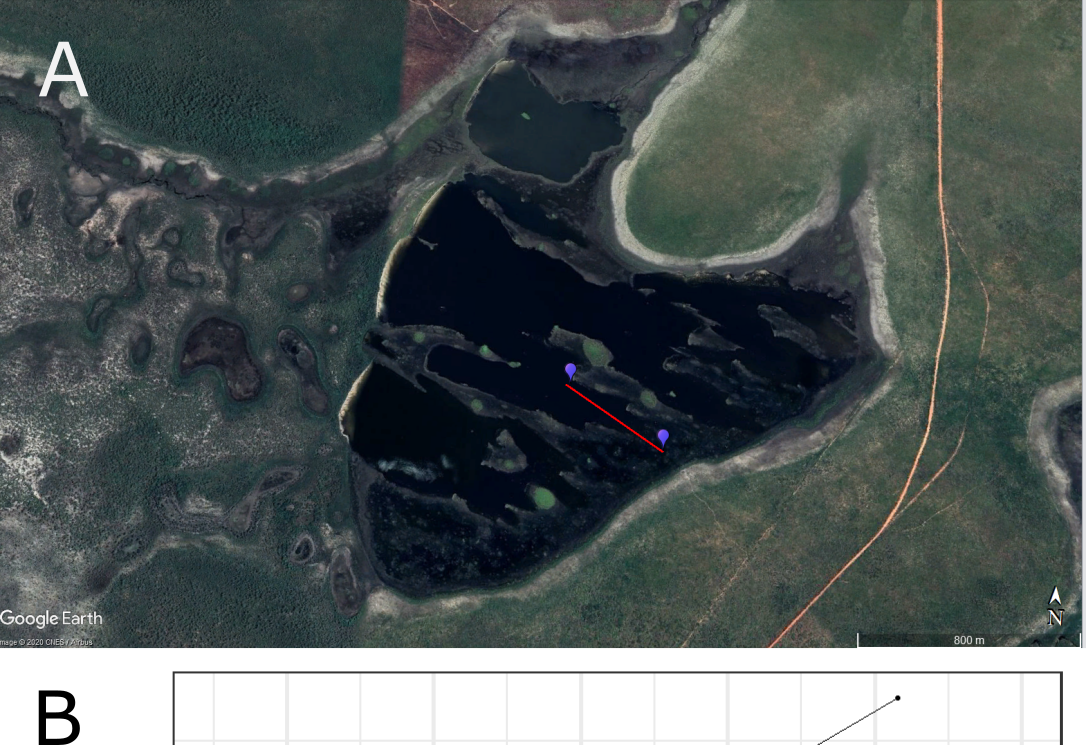
\includegraphics[width=0.8\linewidth]{C:/Users/Maria Jose Rivera/Documents/PhD/Figs/depth_transect_2} 

}

\caption{A) Satellite image of Sanamere showing the transect of surface sampling, B) Cross section of depths across Sanamere Lagoon}\label{fig:depth}
\end{figure}



\hypertarget{methods}{%
\section{Methods}\label{methods}}

\hypertarget{core-processing}{%
\subsection{Core processing}\label{core-processing}}

We returned the core sections to the cold room (4--5 °C) in the Advanced Analytical Centre at James Cook University, Cairns. We opened the core tubes longitudinally, photographed the core sections, and described sediment colors (Munsell) and textures using standard methods \citep{schnurrenbergerClassificationLacustrineSediments2003}. Subsequently, each core section was divided into three slices and each one was sub-sampled at 1 cm intervals. Two slices were stored frozen and intact for ITRAX analyses and archive purposes. The wet weight was recorded, samples were freeze-dried, and the `dry' weight was also recorded for use in calculation of bulk density. One section of each core was scanned using the ITRAX micro X-ray Fluorescence (𝜇XRF) core scanner at the Australian Nuclear Science and Technology Organisation (ANSTO). The scans included optical and X-ray photographs of all sections.

\hypertarget{basic-physical-parameters}{%
\subsection{Basic physical parameters}\label{basic-physical-parameters}}

The physical parameters were calculated following standard guidelines according to \citet{hakansonPrinciplesLakeSedimentology1983}.

\hypertarget{water-content}{%
\subsubsection{Water content}\label{water-content}}

The water content was calculated as the ratio of the weight of water (W), Ww in g, to the dry weight of solids, Ws in g:

\(W = \frac{Ww}{Ws} = \frac{Wt-Ws}{Ws}*100\)

where Wt = the total wet weight (in g)

\hypertarget{dry-bulk-density}{%
\subsubsection{Dry bulk density}\label{dry-bulk-density}}

Bulk density was determined by weighing the wet samples secured from known volumes, oven-drying the material, and re-weighing the sample, according to the following formulas \citep{taylorProceedingsOceanDrilling1992}:

\(p = \frac{Ms}{V}\)

\(p = \frac{M-Mw}{V}\)

where M= total mass of soil, Ms = the mass of the dry sample (weight of the solid portion of the sample), Mw = mass of water and V = the total volume

\hypertarget{grains}{%
\subsubsection{Grain size}\label{grains}}

Forty-two sediment samples, with a sample interval of 4 cm were dispersed with sodium hexametaphosphate and sieved at \textless{} 1000 \(\mu\)m. The \textless{} 1000 \(\mu\)m fraction was subsequently pretreated with 30 \% hydrogen peroxide to remove organics and finally with 1 M NaOH to dissolve biogenic silica, leaving a clastic particulate residue for particle size determination. All pretreated samples were analysed using a Malvern Mastersizer 2000 laser diffraction spectrophotometer. The median grain size and the percentages of clay (\textless{} 2 \(\mu\)m), silt (\textgreater{} 2 \(\mu\)m and \textless{} 63 \(\mu\)m) and sand (\textgreater{} 63 \(\mu\)m) were obtained for each sample \citep{geeParticlesizeAnalysis1986}. Additionally, the percentage of coarse sand (\textgreater{} 275 \(\mu\)m, \textless{} 1000 \(\mu\)m) was also calculated. A correlation matrix between grain size and elemental concentrations was calculated to explore the relationships between these variables. Variability in grain size can indicate changing transport energy, lake levels, and/or the amount and energy of runoff into a sedimentary basin. The presence of larger grains in the sediment record indicates either increased precipitation (especially in closed-basin lake catchments) \citep{chenEnvironmentalRecordsLacustrine2004, conroyHoloceneChangesEastern2008} or lower lake levels resulting from higher accumulation of the nearshore components and/or weaker monsoon circulation in tropical settings \citep{xiaoHoloceneWeakMonsoon2009}.

\hypertarget{basic-chemical-parameters}{%
\subsection{Basic chemical parameters}\label{basic-chemical-parameters}}

\hypertarget{carbon1}{%
\subsubsection{Carbon}\label{carbon1}}

A representative aliquot of each freeze-dried sample was homogenized using a mortar and pestle. An aliquot of each sample (1--10 mg) was weighed into a tin capsule and crimped. The presence of carbonates was checked by comparing the measurements of a batch of 30 samples where carbonates were removed by acid with the results from the untreated batch. No differences were found between the two batches. Total organic carbon and nitrogen abundance and isotope composition of an aliquot of each (1--10 mg) were determined using a Costech elemental analyser fitted with a zero-blank auto-sampler coupled via a ConFloIV to a ThermoFinnigan DeltaV PLUS using continuous-flow isotope ratio mass spectrometry (EA-CF-IRMS) at James Cook University's Cairns Analytical Unit. Stable isotope results are reported as per mil (‰) deviations from the VPDB and AIR reference standard scale for \(\delta\)\textsuperscript{13}C and \(\delta\)\textsuperscript{15}N values respectively. Uncertainty on internal standards (`Low Organic Carbon' \(\delta\)\textsuperscript{13}C −26.54 ‰, \(\delta\)\textsuperscript{15}N 7.46 ‰; `Taipan' \(\delta\)\textsuperscript{13}C -11.65 ‰, \(\delta\)\textsuperscript{15}N 11.64 ‰; and `Chitin' \(\delta\)\textsuperscript{13}C −19.16 ‰, \(\delta\)\textsuperscript{15}N 2.20 ‰) was better than ± 0.1 ‰. Repeated measurements on samples showed that C and N concentrations were generally reproducible to ± 1 \% (1\(\sigma\)).

\hypertarget{silicon-titanium-iron}{%
\subsubsection{Silicon, Titanium, Iron}\label{silicon-titanium-iron}}

XRF elemental profiles were completed for the four sections of the divided core (0-50, 50-100, 100-150, 150-172 cm), for a total of 172 cm, using the second-generation ITRAX core scanner located at the Australian Nuclear Science and Engineering Organisation. Operating conditions for XRF were 40 kV and 30 mA, step size 1000 μm and 10 seconds count time. The XRF scans produced data for a total of 25 elements and were performed using a chromium (to scan Al, Si, P, S, Cl, K, Ca, Sc, Ti, V, Cr) and molybdenum tube set (to scan Mn, Fe, Ni, Cu, Zn, Br, Rb, Sr, Y, Zr, Pd, Ba, La, Ce, Pb). Further information and statistical analyses are included in chapter 5. Optical and radiographic images were also taken of each core using the ITRAX scanner, during XRF scanning. Processing of ITRAX data was completed by ANSTO Facility Officer Dr.~Patricia Gadd. ITRAX elemental counts were normalized using the procedure outlined by \citet{rothwellNewTechniquesSediment2006} and \citet{weltjePredictionGeochemicalComposition2015}. In brief, elements of interest were selected their counts were divided by the total number of counts for that depth. More details about the methodology are available in chapter 5.

In this chapter the results of only three elements (Ti, Fe, Si) are shown, for the purposes of introducing the core stratigraphy.

\hypertarget{results}{%
\section{Results}\label{results}}

\hypertarget{core}{%
\subsection{Core description}\label{core}}

The sedimentary sequence for the Sanamere Lagoon is shown in Figure \ref{fig:fig1} and Table \ref{tab:tb-sed}. Four initial stratigraphic zones were identified based on variations in the basic physical and chemical parameters along the core. The core description will follow a sequence starting at the bottom of the core, with the last section referring to the top of the core. The first layer (172 cm - 140 cm) consists of a dark brown colour (5 YR 5/8), with carbon content below 0.5 \%. Over the interval from 140 to 65 cm mineral content gradually decreases and the colour is light brown (7.5 YR 4/3). A series of three orange (7.5 YR 6/8) 1-cm thick bands are evident over 71 cm - 65 cm (Figure \ref{fig:bands}). Beginning at 65 cm, there is a marked decrease in organic content to values of 0.5 and 1 \% over 43 cm and the sediment colour changes to reddish brown (5 YR 4/4). The upper 43 cm of the core consists of black (10YR 2/1), organic (5 \% - 40 \% carbon) sediments, including the presence of decomposed organic debris.

\begin{figure}

{\centering \includegraphics[width=1\linewidth]{C:/Users/Maria Jose Rivera/Documents/PhD/other/Depth_str_chap_5} 

}

\caption{Stratigraphy of the Sanamere sediment core}\label{fig:fig1}
\end{figure}



\begin{figure}

{\centering 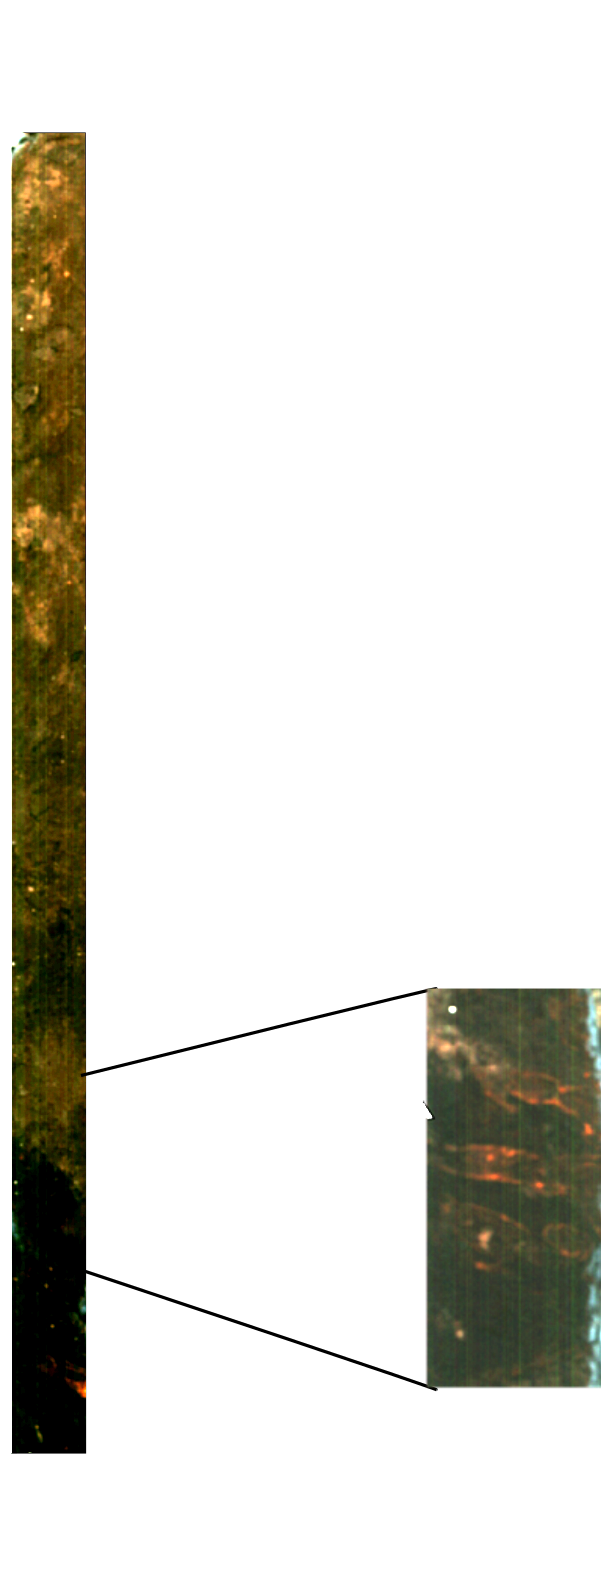
\includegraphics[width=0.8\linewidth]{C:/Users/Maria Jose Rivera/Documents/PhD/Figs/Background/orange_bands_4} 

}

\caption{Orange bands in the Sanamere core}\label{fig:bands}
\end{figure}



\hypertarget{physical-parameters}{%
\subsection{Physical parameters}\label{physical-parameters}}

\hypertarget{water-content-1}{%
\subsubsection{Water content}\label{water-content-1}}

The water content in the sediment column varies between 70.5 \% and 24.4 \%. For the first three stratigraphic units (172 - 43 cm) the percentage stays between 24.4 \% and 36 \%. Starting at 43 cm (46 \%) and until 26 cm, (63 \%) there is a steep increase in water content, from which point it starts to drop to reach 36 \% at 11.5 cm (Figure \ref{fig:fig1}).

\hypertarget{dry-bulk-density-1}{%
\subsubsection{Dry bulk density}\label{dry-bulk-density-1}}

Dry bulk density varies between 0.02 and 1.1 g cm\textsuperscript{-3}. Between 172 cm and 43 cm values remained between 1.1 and 0.71 g cm\textsuperscript{-3}, starting to drop abruptly at 43 cm decreasing to the surface (Figure \ref{fig:fig1}).

\hypertarget{grain-size}{%
\subsubsection{Grain size}\label{grain-size}}

Clastic material of less than 35 \(\mu\)m dominates most of the Sanamere sequence. Between 172 cm and 140 cm, very fine silt (6 - 10 \(\mu\)m) dominates the sequence. An abrupt increment in clay occurs at 136 cm, where clay (\textless{} 2 \(\mu\)m) increases to 45 \%, while silt drops to 55 \%. Between 140 cm and 43 cm, the sand percentage fluctuates between 2 \% and 18 \%, with the only exception at 65 cm, where it increases to 32 \%. At 43 cm, the median grain size, sand and silt percentages increase and the clay percentage decreases. Sand surpasses clay at 38 cm and keeps increasing to the top of the core (Figure \ref{fig:fig1}).

\hypertarget{chemical-parameters}{%
\subsection{Chemical parameters}\label{chemical-parameters}}

\hypertarget{carbon-and-nitrogen}{%
\subsubsection{Carbon and Nitrogen}\label{carbon-and-nitrogen}}

The abundance of carbon percentage varies between 0.3 \% and 41 \% along the entire core. Values fluctuate between 0.32 \% and 1.10 \% between 172 cm and 43 cm, from where they start to increase until they reach 41 \% at 26 cm. From 26 cm, they decrease gradually until the top of the core. The nitrogen percentage values range between 0.03 \% and 1.5 \%. Between 172 cm and 44 cm, they fluctuate between 0.03 \% and 0.2 \%, to then increase gradually to 1.1 \% at 37 cm, where they gradually decrease to 0.3 \% at 5.5 cm, with the exceptions of two high values (1.5 \%) at 4 cm and 4.5 cm (Figure \ref{fig:fig1}). Nitrogen and isotope (carbon and nitrogen) abundances will be discussed in chapters 5 and 6.

\hypertarget{silicon-titanium-iron-1}{%
\subsubsection{Silicon, Titanium, Iron}\label{silicon-titanium-iron-1}}

Complete analysis and interpretation of the ITRAX record is performed in Chapter 5. High water content and low elemental counts prevented the use of the XRF scanning results from 7 cm to the top of the core. The description of Si, Ti and Fe is included in this section to support interpretation in chapter 4. Between 172 cm - 71 cm, the Ti counts stayed relatively constant with minor fluctuations (0.68 - 0.80). After 65 cm, the Ti counts fluctuate and decrease abruptly to 0.01 at 31 cm. From 31 cm, counts increase steadily again to the top of core (Figure \ref{fig:fig-ele}).

Between 172 cm and 140 cm there is minor fluctuations in the Si counts, with low values (0 - 0.07) dominating until 43 cm. Si values start to fluctuate between 0 and 0.32 until the end of the core. They increase rapidly to reach 0.32 at 26 cm (the highest value), to then decrease gradually to reach 0 counts at 18 cm. Finally, counts increase to 0.1 at 8 cm.

The Fe counts are highly consistent (0.95) until 43 cm from where they drop abruptly. Between 43 cm and 22 cm, they fluctuate (0.76 - 0.95). After this period, they increase and keep fluctuating between 0.41 and 1 between 18 cm and 9 cm.

\hypertarget{chapter-3-summary}{%
\section{Chapter 3 summary}\label{chapter-3-summary}}

The Sanamere core consists of a 1.72 m continuous sediment sequence with no evidence that the sedimentary sequence has dried out. The first layer (172 cm - 140 cm), is organic poor and very fined grained with moderate bulk density transitioning to an interval from 140 cm to 65 cm that is similar to the previous one unit, with lighter-coloured sediment and slightly coarser grains. This layer contains three orange bands between 71 and 65 cm. The unit between 65 - 43 cm changes to a reddish-brown color, with increased organic content. The unit between 43 - 0 cm is organic rich, with low bulk density as well as increased grain size and higher water content. High counts of Ti and Fe and low counts of Si dominated the core between 172 - 43 cm and a reverse trend is apparent for the top 43 cm. The following chapter deals with the dating of the sediment core.

\begin{table}

\caption{\label{tab:tb-sed}Layers and units for the Sanamere core}
\centering
\begin{tabular}[t]{ccc}
\toprule
Depth (cm) & Description & Layer\\
\midrule
0-43 & 2.5 YR 4/6 Dark silty peat & 4\\
43-65 & 5 YR 4/4 Silty clay & 3\\
65-140 & 7.5 YR 4/3 Silty clay & 2\\
140-172 & 5YR 5/8 Silty clay with gravel & 1\\
\bottomrule
\end{tabular}
\end{table}



\begin{figure}

{\centering 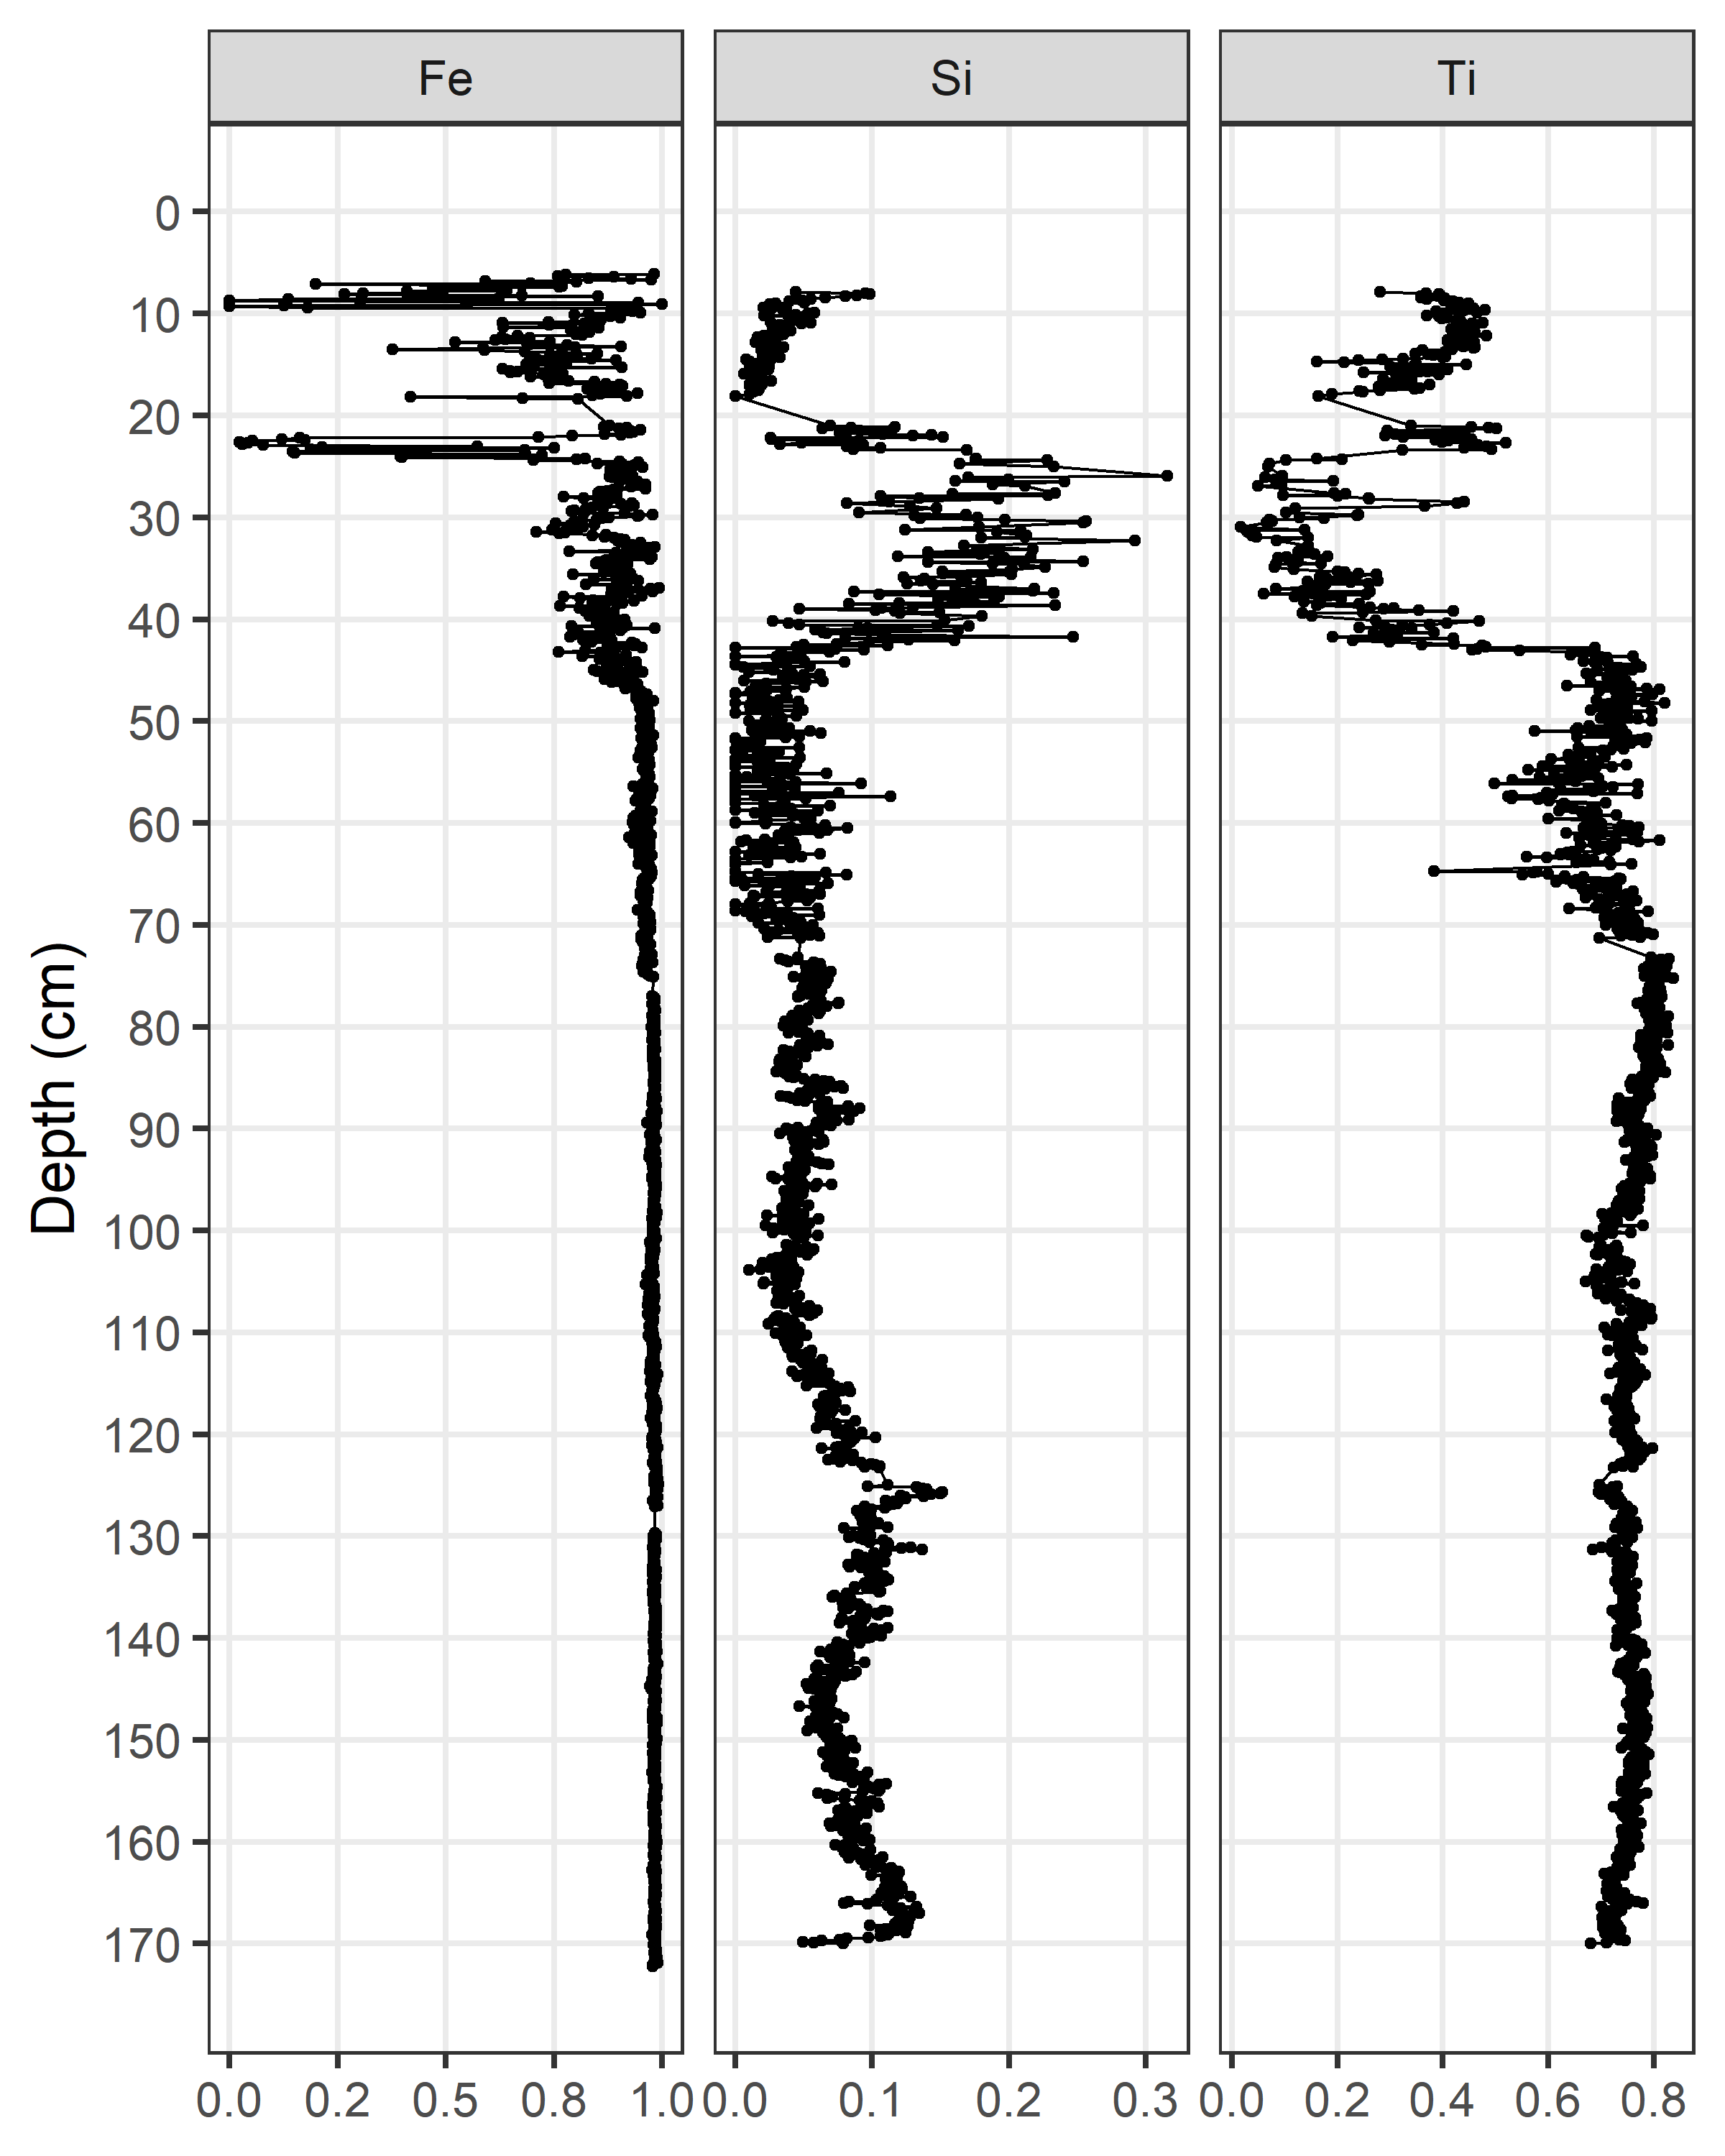
\includegraphics[width=0.8\linewidth]{C:/Users/Maria Jose Rivera/Documents/PhD/Figs/ele_fig} 

}

\caption{Elemental counts in the Sanamere sequence}\label{fig:fig-ele}
\end{figure}



\hypertarget{ch:radiocarbon}{%
\chapter{Developing a radiocarbon chronology for the Sanamere Lagoon sediment core}\label{ch:radiocarbon}}

\hypertarget{introduction-1}{%
\section{Introduction}\label{introduction-1}}

Obtaining an accurate chronology is fundamental to placing any reconstruction of past environmental change within a robust temporal framework. Selecting a reliable carbon fraction and a pre-treatment that removes all or most of the contaminants are key to obtaining reliable radiocarbon dates \citep{pettittPalaeolithicRadiocarbonChronology2003, bronkramseyRadiocarbonDatingRevolutions2008}. This selection becomes particularly challenging in the tropics where high annual temperatures negatively and differentially influence the preservation of different organic fractions. Furthermore, the seasonal nature of the tropical hydrological cycle in northern Australia results in high rates of weathering and variable pH and redox conditions, in turn altering carbon cycling and preservation in lake sediment columns \citep{birdRadiocarbonAnalysisEarly2002, highamRadiocarbonDatingCharcoal2009}. Collectively, these conditions limit the availability of those organic components considered more reliable and the dating of other fractions can result in aberrant radiocarbon results that are linked to, for example, poorly preserved or degraded charcoal, identifiable when the combustion yields are lower than usually expected (50--60 \% carbon by weight) \citep{highamRadiocarbonDatingCharcoal2009}. Although there is currently no agreement about which is the most reliable fraction to avoid these issues, short-lived plant macrofossils and charcoal \citep{cohenPaleolimnologyHistoryEvolution2003, martinRadiocarbonAgesDifferent2019} tend to be among the most favoured materials for dating.

Despite the importance of choosing a reliable carbon fraction that represents the age of contemporaneous sediment deposition, few studies have focused on sediments in the tropics. Comparative studies based on multiple organic fractions in the tropics have focused on swamps \citep{mayEstablishingChronologicalFramework2018}, peats \citep{wustComparisonRadiocarbonAges2008} and organic springs \citep{fieldUntanglingGeochronologicalComplexity2018}, with no studies having been undertaken using lake sediments and no studies in any tropical environment compare more than four fractions. Results from the available studies (as mentioned above) are contradictory regarding the reliability of macro-charcoal and pollen concentrates (yielding anomalously older or younger ages compared to other fractions). Studies in temperate areas have also reported significant discrepancies between radiocarbon dates for different, supposedly contemporaneous carbon fractions in lake sediments from the same depth. For example, in boreal and arctic lake sediments wood and charcoal were found to be older than other organic materials such as conifer and deciduous periderms, usually by several hundred years \citep{oswaldEffectsSampleMass2005}.

Discrepancies have likewise been found within different types of macrofossils, with some more prone to an apparent `reservoir effect' \citep{turneyImplicationsDatingWisconsinan2000}. For instance, pollen, charcoal and bulk sediment are recognized to be highly mobile, porous and heterogeneously sourced, all of which complicates their reliability for radiocarbon dating. Additionally, several studies have demonstrated that there are significant uncertainties associated with simply dating bulk sediment, regardless of the geographical location from where the sample was collected \citep{bjorckHighresolution14CDated1998, wustComparisonRadiocarbonAges2008, xuVariationsRadiocarbonAges2003}. Extensive research has shown how the effect of contamination depends on the age of the sample \citep{pettittPalaeolithicRadiocarbonChronology2003, highamRadiocarbonDatesOxford2011, woodRevolutionConventionPresent2015}. Dating beyond 10 thousand calibrated years before present (ka) becomes considerably more problematic as even minimal percentages of contamination can cause hundreds to thousands of years of offset \citep{aitkenSciencebasedDatingArchaeology1990, woodRevolutionConventionPresent2015}. In fact, offsets of up to 16,000 years between radiocarbon ages from bark and pollen from a tropical peat were obtained in a previous study, with pollen extracts resulting in older dates \citep{wustComparisonRadiocarbonAges2008}.

Pre-treatment procedures are also fundamental to the generation of accurate radiocarbon dates. While acid-base-acid (ABA treatment) is routinely employed to remove contaminants, it is not always effective \citep{chappellRadiocarbonLimitAustralian1996, gillespieAMSDatingLate1992}. Notably, the determination of when decontamination is complete is technically challenging. The base treatment during ABA can further remove charcoal by solubilizing it to `humic acid', resulting in considerable sample loss. As an alternative to ABA, acid-base-wet oxidation (ABOX) has been found to be more appropriate and an effective method to remove contamination, especially for old samples \citep{birdRadiocarbonDatingOld1999, birdEfficiencyCharcoalDecontamination2014}. However, the harshness of the technique can remove excessive carbon and this may limit the application of the technique in the tropics where macroremains are scarce \citep{birdRadiocarbonDatingOld1999}. Recent studies have shown that ABA and hypy-treated pairs can produce comparable results to each other in some contexts \citep{birdEfficiencyCharcoalDecontamination2014, alexRadiocarbonChronologyManot2017, david45610522019}. Hydropyrolysis (hypy) (to isolate stable polycyclic aromatic carbon: SPAC) has shown promising results in mound spring deposits, where the technique appeared to remove the effects of post-depositional modification to the ages obtained from different organic fractions from the sediment \citep{fieldUntanglingGeochronologicalComplexity2018}. Given this promising result, hypy pretreatment might be expected to be similarly effective in lake sediments.

Given the fact that most studies rely on the dates from one organic fraction over the entire sequence, it is imperative to test whether alternative protocols using different carbon fractions, pre-treatments would yield more accurate results across a range of depositional ages. This chapter examines six carbon fractions in samples from a Sanamere Lagoon sediment core to determine which fraction and technique pre-treatment is most appropriate to obtain reliable radiocarbon dating results.

\hypertarget{methodology}{%
\section{Methodology}\label{methodology}}

Details about the site, field work and core processing can be found in chapter \ref{ch:sed}. Samples for \textsuperscript{14}C AMS dating were obtained for six different carbon fractions (hypy, microcharcoal, macrocharcoal, pollen concentrate, `cellulose' and bulk organics) for six depths spread along the core (Table \ref{tab:tb-one}, Figure \ref{fig:radiocarbonmet} and Figure \ref{fig:fractions}). These depths were chosen by consideration of the stratigraphic changes (see chapter \ref{ch:sed}) observed along the sequence (texture, color, elemental abundance). Although attempts to extract all fractions from the same depth were made, this was not achieved as samples from some depths yielded insufficient amounts of carbon after pretreatment to be processed for radiocarbon dating (Appendix 1). In order to address this issue, samples from additional depths were analysed to complete the age-depth model.

\hypertarget{pre-treatment}{%
\subsection{Pre-treatment}\label{pre-treatment}}

Pre-treatment of radiocarbon samples for pollen, cellulose, macrocharcoal, microcharcoal and bulk organics (standard method) followed the ANSTO protocols detailed below.

\hypertarget{pollen}{%
\subsubsection{Pollen}\label{pollen}}

Extraction of pollen was adapted from \citet{bennettPollen2002}. Three sediment samples were washed with 10 \% HCl and then passed through a 150 \(\mu\)m sieve. The smaller fraction was retained and then washed with 10 \% NaOH several times until the supernatant was clear. Subsequently, 20 mL of 40 \% HF was added and the sample left overnight. Subsequently, the samples were first washed two times with 2 M HCl and finally with Milli-Q water. Lithium heteropolytungstate (LST) with a specific gravity of 1.8 was used for density separation, with the floating fraction retained for examination under the microscope. The resultant pollen concentrate was dried overnight at 60°C.

\hypertarget{bulk-organics-standard-method}{%
\subsubsection{Bulk organics (standard method)}\label{bulk-organics-standard-method}}

Five sediment samples were processed at ANSTO following the ABA pre-treatment detailed in \citet{hatteClassicalAcidAlkaliAcidTreatment2001}. First, visible contaminants (roots, rocks) were removed and then a wash with 2 M HCl was performed (to remove carbonates), followed by sequential washes of 0.5 \%, 1 \%, 2 \% and 4 \% NaOH, until the supernatant liquid was clear (to remove fulvic and humic acids). A wash with 2 M HCl to remove any atmospheric carbon dioxide (CO\textsubscript{2}) absorbed during alkali treatment was performed, followed by three washes with Milli-Q water, and the samples were finally oven-dried at 60 °C overnight.

\hypertarget{bulk-organics-modified-method}{%
\subsubsection{Bulk organics (modified method)}\label{bulk-organics-modified-method}}

The pretreatment with hydrogen peroxide has proven to be effective in removing contaminant organic matter in radiocarbon dating samples \citep{chiuExtendingRadiocarbonCalibration2005}. In order to further test the success in removing exogenous organic matter, two additional sediment samples were first pretreated with 30 \% hydrogen peroxide overnight at the Advanced Analytical Centre at James Cook University Cairns, freeze dried and then sent for standard ABA pre-treatment at the Waikato Radiocarbon Dating Laboratory. This procedure involved the removal of visible contaminants, following with the samples washed with hot HCl, then rinsed and treated with multiple hot NaOH washes. The NaOH insoluble fraction was treated with hot HCl, filtered, rinsed and dried.

\hypertarget{macro-and-microcharcoal}{%
\subsubsection{Macro and microcharcoal}\label{macro-and-microcharcoal}}

Charcoal samples at 6 cm were pre-treated with 30 \% hydrogen peroxide for 2 h and then passed through 250 \(\mu\)m and 63 \(\mu\)m sieves. These two fractions were then examined under the microscope, and pieces of charcoal were recovered using tweezers (in the case of the \textgreater250 \(\mu\)m fraction) and an Eppendorf InjectMan® 4 micromanipulator (for the 63 - 250 \(\mu\)m fraction). Samples were then washed with 0.5 \% NaOH and 2 M HCl. Samples at 3 and 82 cm were pre-treated with 10 \% hydrogen peroxide and the pre-treatment followed as above.

\hypertarget{cellulose}{%
\subsubsection{Cellulose}\label{cellulose}}

Extraction of cellulose was adapted from \citet{gillespieNovelCellulosepreparationMethod2019}. Three sediment samples were pre-treated with 1 M NaOCl/NaOH for 2 hours and washed with 1 M HCl. The samples were then reacted with 1 M NaClO\textsubscript{2}/HCl for another 2 hours and then washed with 1 M HCl. This procedure was then repeated and the samples were washed with water three times. Finally, samples were oven-dried at 60°C overnight.

\hypertarget{hypy-fraction}{%
\subsubsection{Hypy fraction}\label{hypy-fraction}}

Fourteen sediment samples were pretreated using hypy to isolate the pyrogenic carbon (PyC) \citep{ascoughHydropyrolysisNewTool2009, meredithAssessmentHydropyrolysisMethod2012}. First, 30 \% hydrogen peroxide was added to the samples. The samples were left overnight then washed with 2 M HCl, and freeze dried. Aliquots of each sample were then loaded with a catalyst and 20 \% MeOH/H\textsubscript{2}O solution, sonicated for 15 min and dried over a hotplate at 60 °C. These samples were placed in the HyPy reactor, pressurized with hydrogen (H\textsubscript{2}) to 150 bar with a gas flow of 4 L/minute over 40 minutes. Finally, samples were washed for 2 hours with 6 M HCl at 60 °C.

\hypertarget{graphitization-and-measurement}{%
\subsection{Graphitization and measurement}\label{graphitization-and-measurement}}

Samples were combusted at 900 °C to convert them to CO\textsubscript{2}, followed by graphitisation using the H\textsubscript{2}/Fe method \citep{huaProgressRadiocarbonTarget2001}. Carbon-14 measurement of all samples was undertaken by Accelerator Mass Spectrometry (AMS) on the VEGA and ANTARES accelerators at ANSTO \citep{finkANTARESAMSFacility2004} except for samples Wk50327 and Wk50328, which were measured at the Waikato Radiocarbon Dating Laboratory.

\hypertarget{calibration}{%
\subsection{Calibration}\label{calibration}}

All samples were calibrated using the rbacon R package \citep{blaauwRbaconAgedepthModelling2019} and the IntCal13 calibration curve \citep{reimerIntCal13Marine13Radiocarbon2013} with 0 calibrated years before present representing 1950 AD. IntCal13 was used rather than SHCal13. IntCal13 was used due to the influence of Northern Hemisphere air masses on the Tropical North of Australia, when the Inter Tropical Convergence Zone moves southwards during the Australian-Indonesian summer monsoons \citep{hoggSHCal13SouthernHemisphere2013}.

\begin{figure}

{\centering \includegraphics[width=1\linewidth]{C:/Users/Maria Jose Rivera/Documents/PhD/Figs/SAN_final} 

}

\caption{Sanamere Lagoon on Cape York Peninsula}\label{fig:radiocarbon1}
\end{figure}



\begin{figure}

{\centering 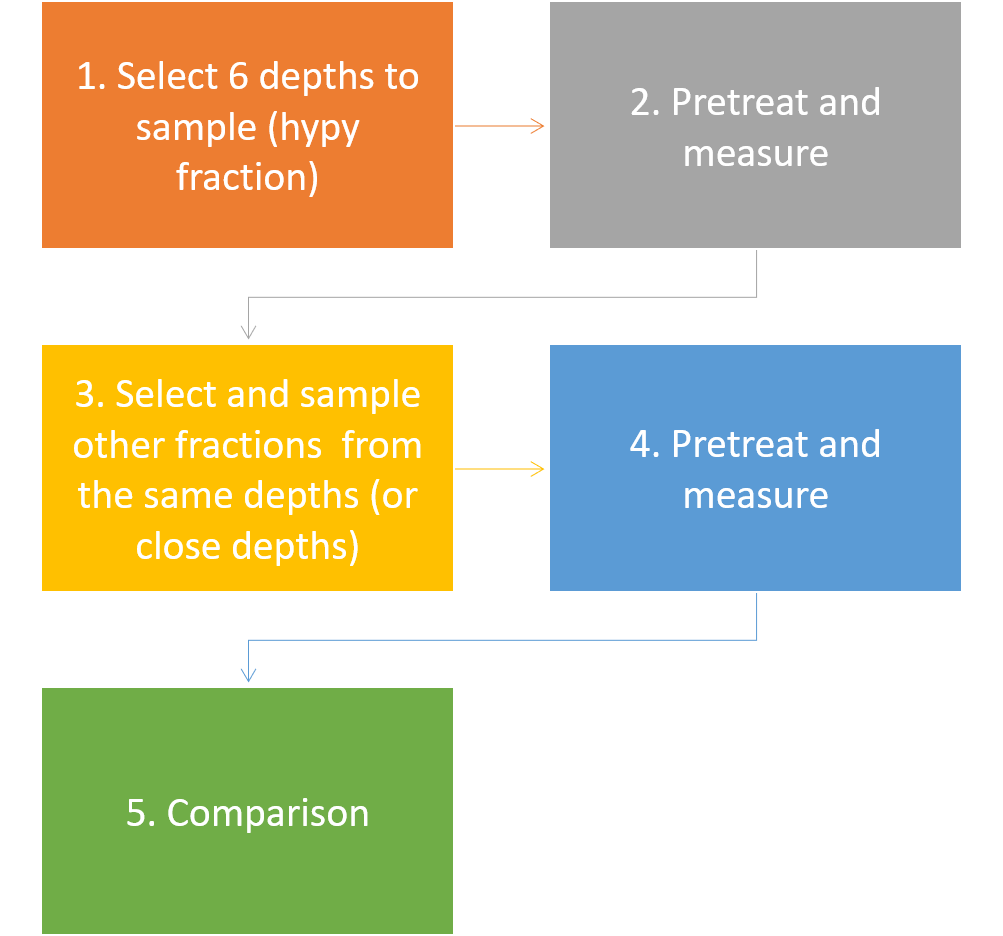
\includegraphics[width=1\linewidth]{C:/Users/Maria Jose Rivera/Documents/PhD/other/RC cha/rad_met} 

}

\caption{Summary of methods}\label{fig:radiocarbonmet}
\end{figure}



\begin{figure}

{\centering 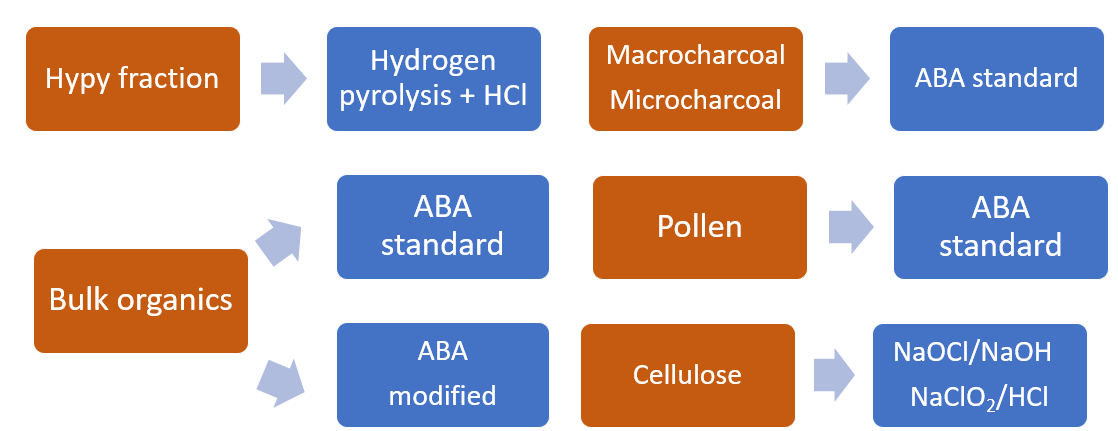
\includegraphics[width=1\linewidth]{C:/Users/Maria Jose Rivera/Documents/PhD/other/RC cha/fractions} 

}

\caption{Carbon fractions and corresponding pretreatment techniques}\label{fig:fractions}
\end{figure}



\hypertarget{results-1}{%
\section{Results}\label{results-1}}



A total of 27 radiocarbon dates were obtained for 17 different depths along the core. Overall, the ages ranged from 2.067 - 2.466 ka (2 \(\sigma\)) at 3 cm (hypy fraction) to 30.889 - 31.304 ka (2 \(\sigma\)) at 162 cm (hypy fraction), spanning 29237 years in total. As discussed above, ages were obtained for more than one fraction from six depths. Table \ref{tab:tb-one} shows the results from the radiocarbon dating measurements and the calibrated results. Below 82 cm, the availability of fractions to compare was reduced to bulk organics, the hypy fraction and pollen concentrates, as these were the only fractions to yield sufficient carbon to be analysed by AMS. Therefore, charcoal fractions \textgreater{} 63 \(\mu\)m and cellulose could not be compared after this depth. From the three depths originally processed with the cellulose pre-treatment method only one sample retained enough carbon to be measured, given the aggressiveness of the pretreatment.

The micro-charcoal result at 3 cm showed the largest age reversal overall, 8,990 years older than the hypy date at the same depth. Two pairs of hypy ages also showed age reversals, with the smallest (a difference of 840 years) between the dates at 23 and 32 cm and the largest between the dates 90 and 105 cm (a difference of 1970 years). The only cellulose sample yielded a younger date in comparison to what was expected for that depth based on the other results (Table \ref{tab:tb-one}, Figure \ref{fig:radiocarbon-gr2}).

The difference between the ages from different fractions generally increased with depth (Table \ref{tab:tb-four}). The only section of the core where all dating results overlap (except for the pollen concentrate) is at 6 cm, while the other five depths showed large differences between the results from different fractions, with the largest offset at 146 cm (a difference of 16,527 years), between hypy and pollen. The bulk organic fractions pretreated with standard ABA procedures also differed significantly from the hypy fraction (being up to 9,516 years younger than the former). Although not from the same depths (but within 10 cm), the modified ABA pretreatment yielded results that aligned closely with the hypy results at the two depths they were compared.

In four out of six cases (the deepest samples), hypy yielded the oldest date from those available at that depth, and in two cases (the shallowest samples), hypy yielded the youngest results. Bulk organics (standard ABA) yielded the youngest result for four depths (43, 67, 137 and 146 cm). The pollen results were inconsistent, yielding the oldest and youngest dates at 6 cm and 146 cm, respectively (Table \ref{tab:tb-four}).

\begin{table}

\caption{\label{tab:tb-one}Conventional and calibrated dates from all samples tested in the study}
\centering
\resizebox{\linewidth}{!}{
\begin{tabular}[t]{lrllll}
\toprule
Laboratory Code & Depth & Conventional radiocarbon dates & Calibrated age range (95 \%) & Carbon fraction & Pretreatment\\
\midrule
OZY416 & 3.0 & 2,270 ± 70 & 2067 - 2466 & SPAC & Hypy\\
OZY423 & 3.0 & 11,260 ± 160 & 12742 - 13368.5 & Charcoal >63 um & ABA\\
OZX672 & 6.0 & 3,840 ± 45 & 4099.5 - 4412 & SPAC & Hypy\\
OZY131 & 6.0 & 4,450 ± 30 & 4894 - 5284.5 & Pollen & ABA\\
OZX765U2 & 6.0 & 4,180 ± 140 & 4243 - 5040 & Charcoal >63 um & ABA\\
OZX765U1 & 6.0 & 4,120 ± 100 & 4296.5 - 4845 & Charcoal >250 um & ABA\\
OZX765 & 6.0 & 4,165 ± 35 & 4580 - 4830.5 & Bulk organics & ABA\\
OZY417 & 12.5 & 4,230 ± 70 & 4535 - 4960 & SPAC & Hypy\\
OZY418 & 23.0 & 7,140 ± 80 & 7798 - 8162 & SPAC & Hypy\\
OZY333 & 32.0 & 6,435 ± 30 & 7292.5 - 7425 & SPAC & Hypy\\
OZY419 & 42.0 & 6,150 ± 80 & 6754.5 - 7239.5 & Cellulose & Gillespie\\
OZX673 & 43.0 & 8,660 ± 40 & 9774 - 10164.5 & SPAC & Hypy\\
OZX766 & 43.0 & 7,750 ± 35 & 8435 - 8594.5 & Bulk organics & ABA\\
OZX674 & 67.0 & 15,240 ± 60 & 18344 - 18670.5 & SPAC & Hypy\\
OZX767 & 67.0 & 9,900 ± 50 & 11208 - 11599.5 & Bulk organics & ABA\\
OZY420 & 76.0 & 17,670 ± 160 & 20929 - 21825.5 & SPAC & Hypy\\
OZY758 & 82.0 & 10,940 ± 110 & 12665.5 - 13036 & Charcoal >63 um & ABA\\
OZY421 & 90.0 & 19,450 ± 80 & 23101.5 - 23685 & SPAC & Hypy\\
OZY422 & 105.0 & 18,350 ± 170 & 21815 - 22540 & SPAC & Hypy\\
Wk50327 & 114.0 & 23,549 ± 126 & 27470 - 27889.5 & Bulk organics & H2O2 + ABA\\
OZX675 & 137.0 & 24,340 ± 190 & 27932.5 - 28765 & SPAC & Hypy\\
OZX768 & 137.0 & 15,560 ± 90 & 18620.5 - 18996 & Bulk organics & ABA\\
OZX676 & 146.0 & 26,290 ± 260 & 29870 - 31010 & SPAC & Hypy\\
OZY132 & 146.0 & 11,920 ± 40 & 13567 - 13944 & Pollen & ABA\\
OZX769 & 146.0 & 16,270 ± 70 & 19449 - 19905 & Bulk organics & ABA\\
Wk50328 & 150.0 & 25,931 ± 167 & 29655 - 30683 & Bulk organics & H2O2 + ABA\\
OZX677 & 162.0 & 27,100 ± 140 & 30889.5 - 31304 & SPAC & Hypy\\
\bottomrule
\end{tabular}}
\end{table}



\begin{table}

\caption{\label{tab:tb-four}Offset, minimum and maximum calibrated ages by depth}
\centering
\resizebox{\linewidth}{!}{
\begin{tabular}[t]{rrlrlrr}
\toprule
Depth (cm) & Minimum age & Carbon fraction (min) & Maximum age & Carbon fraction (max) & Offset & Number of dates\\
\midrule
55 & 18620.5 & Bulk organics & 28765.0 & Hypy & 9540.50 & 2\\
64 & 13567.0 & Pollen & 31010.0 & Hypy & 16684.50 & 3\\
101 & 2067.0 & Hypy & 13368.5 & Charcoal >63 um & 10788.75 & 2\\
104 & 4099.5 & Hypy & 5284.5 & Pollen & 833.50 & 5\\
143 & 8435.0 & Bulk organics & 10164.5 & Hypy & 1454.50 & 2\\
166 & 11208.0 & Bulk organics & 18670.5 & Hypy & 7103.50 & 2\\
NA & 4535.0 & Hypy & 31304.0 & Hypy & 26349.25 & 2\\
\bottomrule
\end{tabular}}
\end{table}



\begin{figure}

{\centering 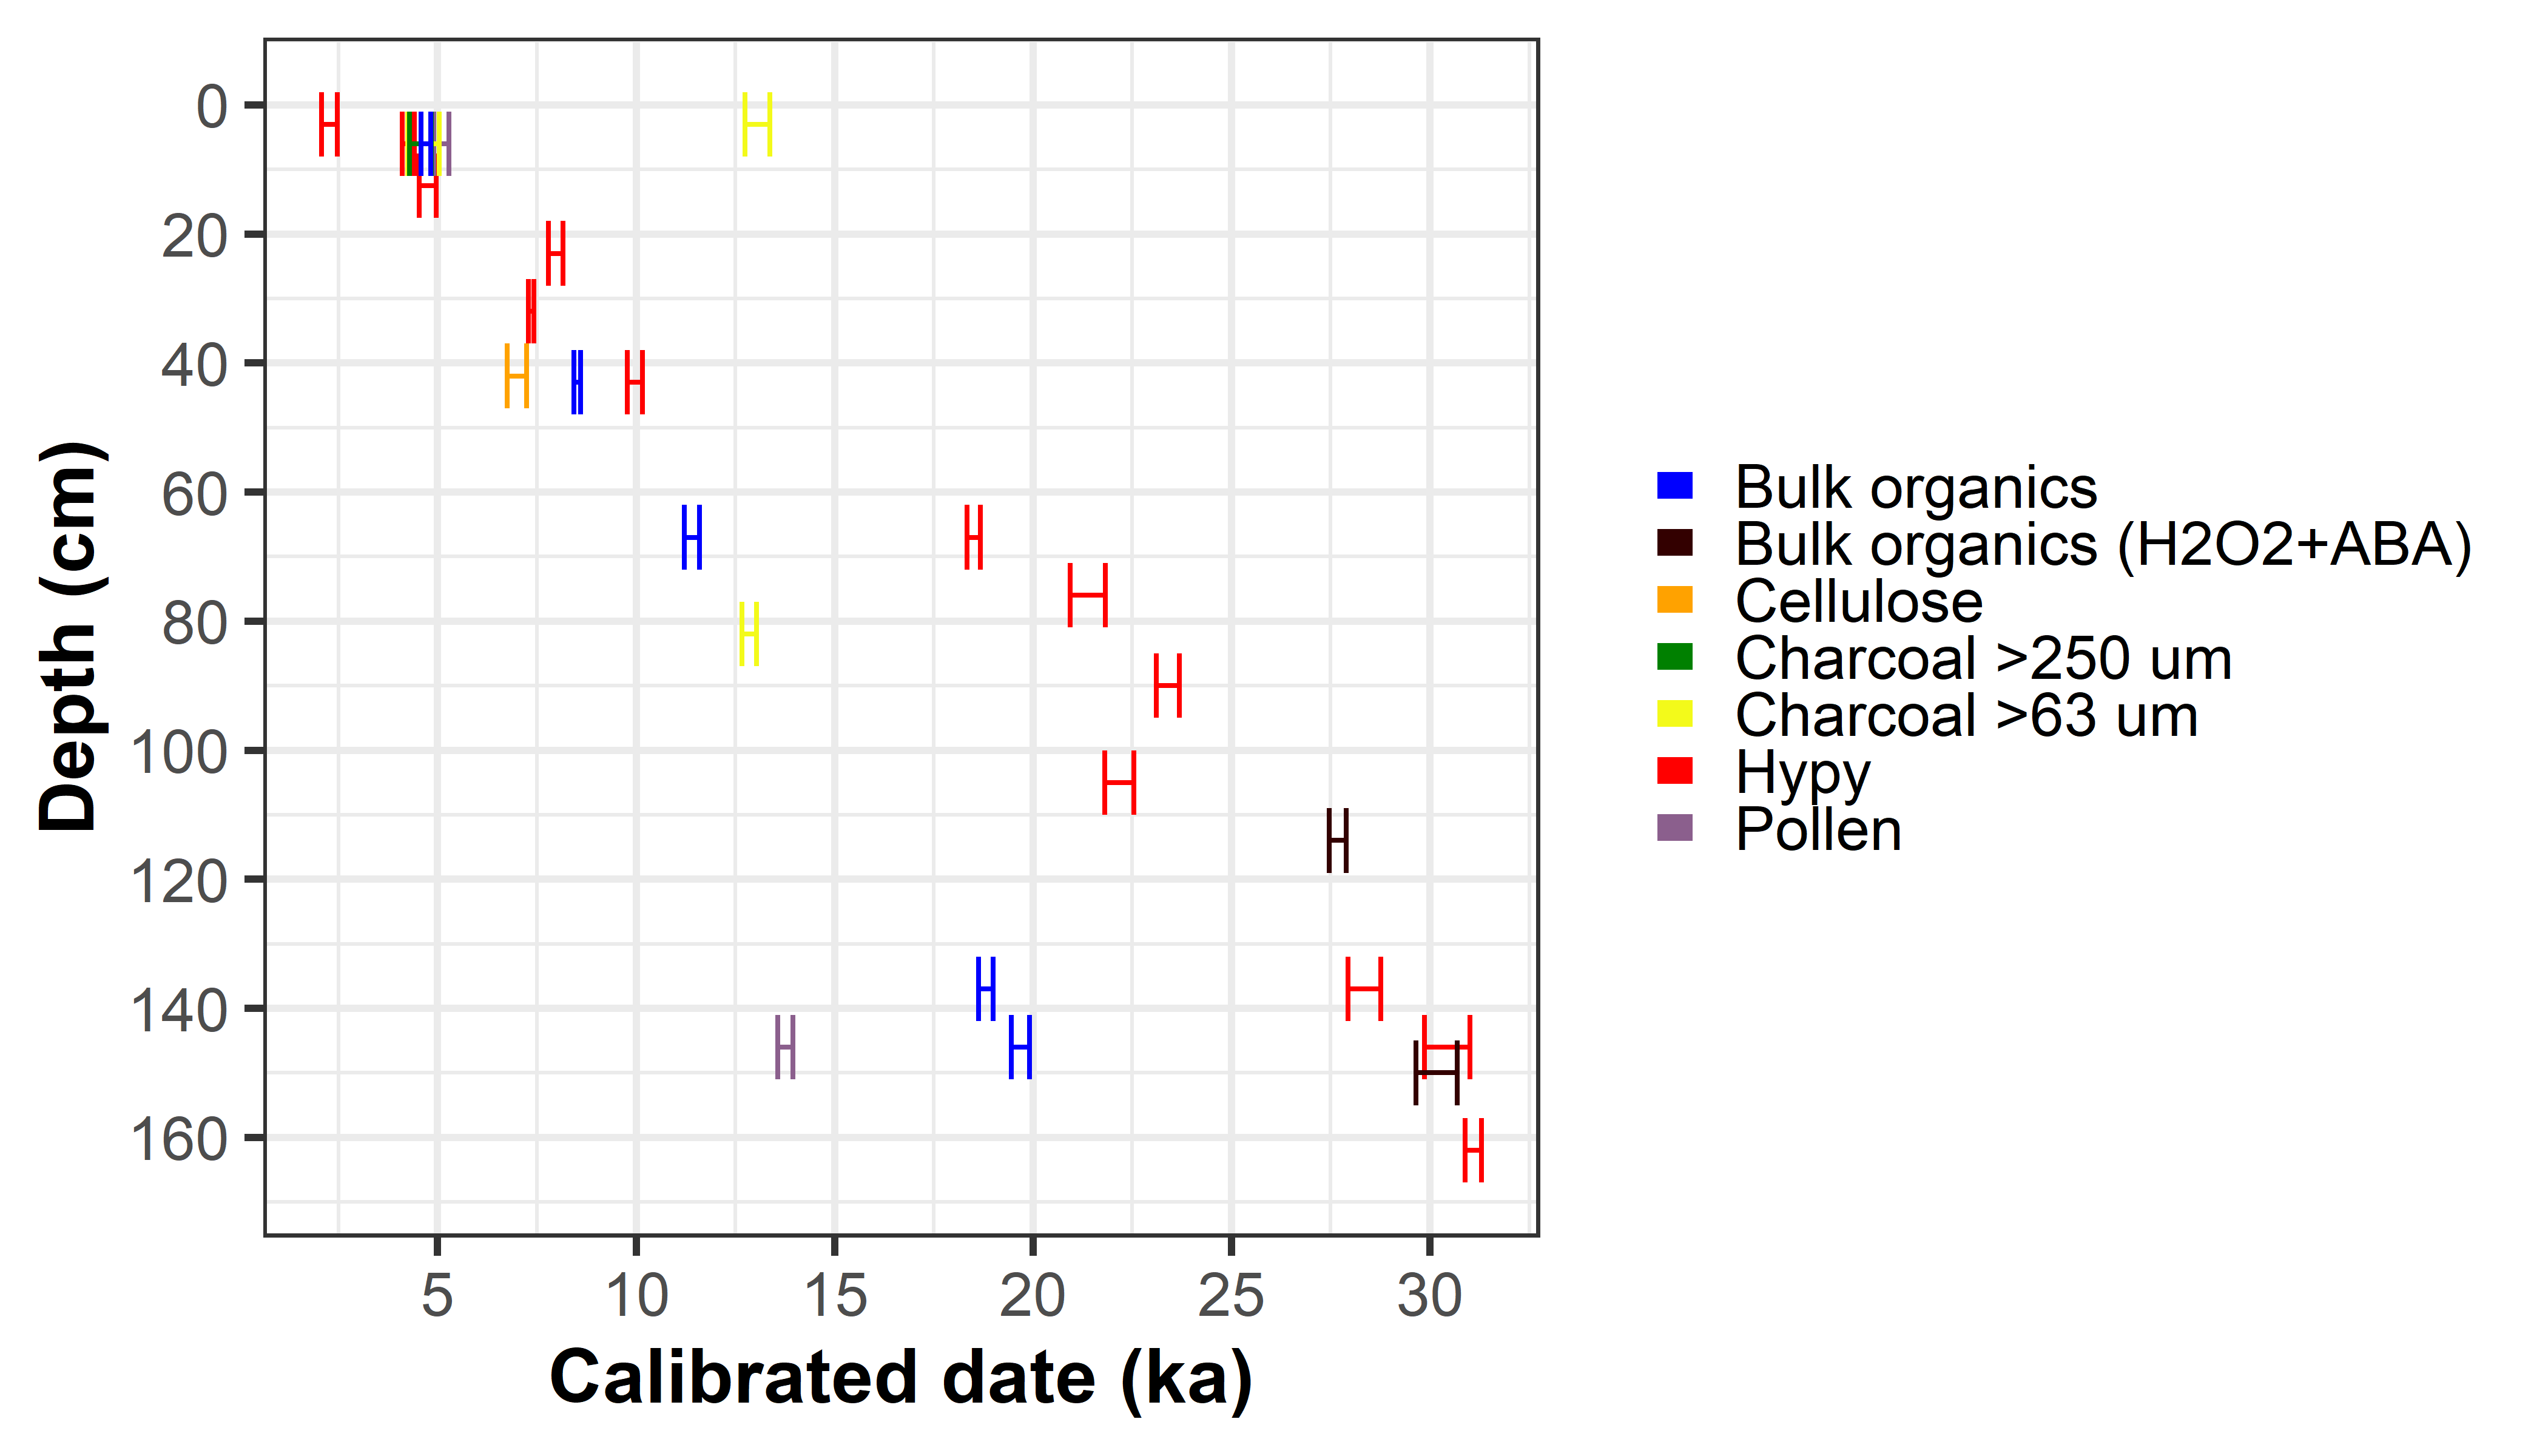
\includegraphics[width=1\linewidth]{C:/Users/Maria Jose Rivera/Documents/PhD/Figs/dates_RC_2} 

}

\caption{Calibrated ages by depth and carbon fraction along the Sanamere sediment core}\label{fig:radiocarbon-gr2}
\end{figure}



\hypertarget{discussion}{%
\section{Discussion}\label{discussion}}

\hypertarget{assessment-of-reliability}{%
\subsection{Assessment of reliability}\label{assessment-of-reliability}}

The hypy dates yielded the oldest dates and the most consistent internal chronology with only two minor age reversals (at 23 and 90 cm). Although previous studies suggest that hypy dates could be biased to older ages due to potential for reservoir effects \citep{fieldUntanglingGeochronologicalComplexity2018}, this study found this pre-treatment and its resulting carbon fraction (SPAC) to be the most reliable.

All ages returned (except at 6 cm) following hypy pre-treatment are considerably older than dates from comparable levels for other carbon fractions. This finding is consistent with the results obtained from the radiocarbon dates from organic spring deposits in northwest Australia, where hypy ages were found to be older than other fractions, but also considered more reliable based on their more consistent age-depth relationship within each core \citep{fieldUntanglingGeochronologicalComplexity2018}. Hypy reduces labile organic matter to volatile products \citep{ascoughHydropyrolysisNewTool2009} and potentially removes \textgreater{} 92 \% of all labile carbon \citep{birdEfficiencyCharcoalDecontamination2014}. Hypy represents the carbon fixed by pyrolysis at the time of a burning event, therefore the `indigenous' or core component of the original charcoal \citep{ascoughHydropyrolysisNewTool2009, ascoughHydropyrolysisImplicationsRadiocarbon2010}.

The hypy dates at 23 cm (7.798 - 8.162 ka) and 32 cm (7.292 - 7.425 ka) show an age reversal of 506 - 870 years (Figure \ref{fig:radiocarbon-gr2}). These dates are from the section of the core that has high organic content, high pyrogenic carbon mass accumulation rates and large fluctuations in the normalized titanium counts (range 0.02 - 0.45). Both changes in erosion (as evidenced by clastic input) and high organic input at this time suggest that some reworking could have happened during this period, which coincides in timing with the flooding of the adjacent continental shelf in response to an increase in sea level during the early Holocene in north Australia \citep{slossHoloceneSealevelChange2018a, chivasSealevelEnvironmentalChanges2001, yokoyamaShorelineReconstructionAustralia2001, reevesPalaeoenvironmentalChangeTropical2013}, and therefore to a period of wetter climate, with potentially more intense seasonal rainfall events. More overland transport of soil material from the catchment, may well have transported `old' charcoal into the lake at this time. A second age reversal is present between results at 90 cm and 105 cm (1,100 years) in the hypy results, with the only apparent sedimentological indication of change being a slight decrease in the titanium counts down-core between these two depths. It is possible that the date at 105 cm exhibits an incomplete removal of exogenous carbon, the main issue identified when applying hypy pre-treatment to charcoal formed at 400°C or below \citep{birdEfficiencyCharcoalDecontamination2014}.

The results from fractions other than hypy at the same or comparable depths (except at 6 cm) were uniformly younger than the hypy results. Besides the possibility of the physical mobility of material in the sediment columns, it is likely that the differences between the ages of fractions at 43, 67, 137 and 146 cm are the result of unremoved contamination by carbon of a different, generally younger age in the bulk organics (standard treatment) and pollen fractions. The mobilization of materials and therefore, the contamination of samples with exogenous carbon is made more likely in the Sanamere sequence because the entire 31,000 years of accumulation is represented in only 172 cm of sediment. The top 43 cm contains high proportions of water, which also facilitates the mixing of materials by physical translocation and/or solubilization.

The results suggest that, for the majority of samples in this study, the standard ABA pretreatment was ineffective in removing modern contamination from the bulk organic fraction. An inbuilt `reservoir' age associated with a period of storage in the lake catchment may have biased the hypy results to older ages by an unknown amount. However, it is unlikely that this could cause such large offsets between the hypy dates and dates from the other fractions. If there was a reservoir offset relating to a period of storage of up to 9,540 years in the catchment, this would manifest itself in the hypy dates throughout the sequence, whereas what is observed is a generally smaller offset up the core. Indeed, the uppermost hypy date the hypy date is younger than that of the other fractions, implying the circulation of carbon of an apparent age representative of all carbon in the sediment through the relatively thin sediment pile, such that dates high in the sequence are biased old and dates deeper in the sequence are biased young.

Further evidence that there is no substantial reservoir effect on the hypy dates is provided by the observation that the two samples subject to the modified bulk organic pretreatment, where peroxide was used before standard ABA yielded results close to those obtained from the hypy fraction. Except for the anomalous charcoal result at 3 cm, and the slightly old pollen date at 6 cm, all dates from all fractions and pretreatments before 23 cm overlapped (when they belonged to the same depth), and did not show any age reversals. Below 23 cm, large offsets between samples from the same depth and age reversals were observed.

The increasing magnitude of the difference between hypy and the other fractions ages with depth/age is consistent with what would be expected for the younger samples having between 2 and 5 \% unremoved modern contamination \citep{woodRevolutionConventionPresent2015}, or more contamination of an older aggregate apparent age.

The results strongly indicate the presence of unremoved exogenous carbon contamination in some of the fractions. For example, the largest offset between two fractions was found at 146 cm (16,685 years) between pollen and hypy, which suggests that pollen from higher depths mobilized down the core and/or the concentrate contained exogenous younger materials. The two pollen concentrate samples available show inconsistent results, as has been found in previous studies (younger \citep{fieldUntanglingGeochronologicalComplexity2018, mayEstablishingChronologicalFramework2018} or older \citep{neuliebPotentialPitfallsPollen2013, fletcherAMSRadiocarbonDating2017}), with the sample at 6 cm having the oldest date compared with the other fractions at the same depth, while the sample at 146 cm is the youngest compared to the bulk organics and hypy results. When inspected under the microscope, these samples appeared to be composed by around 50 \% pollen, with the rest of material being plant material and charcoal. This addition of heterogeneously sourced materials could have added exogenous carbon contamination resulting in the aberrant results. Other studies also have identified anomalous, generally younger ages derived from pollen concentrates \citep{mayEstablishingChronologicalFramework2018, clymoUpwashDownwashPollen1987} due to the high physical mobility of small particles but also the high porosity of the pollen walls, which can sorb and accumulate exogenous carbon \citep{kilianProblematic14CAMSDates2002a}. The existence of clearly anomalously young pollen dates strongly suggests that there is potential for contamination by young carbon in all the organic fractions.

Large offsets (up to 9,504 years) were also found between bulk organics and hypy, with the former showing younger ages. This finding is consistent with previous studies which found that bulk organics pretreated with standard ABA can yield anomalously young dates \citep{wangRadiocarbonDatingSoil1996, wustComparisonRadiocarbonAges2008, pessendaRadiocarbonDatingTotal2001}. Although measured at 42 cm (not 43 cm as the other two fractions), the cellulose extraction yielded an age younger compared to what was expected from the bulk organics and hypy age-depth relationship.

While the results from micro and macro charcoal were expected to be tested along the entire core to better understand differences in their sources, their availability was limited below 82 cm. As the age ranges obtained for both overlapped at 6 cm, the possibility that they represent different sources is low. The charcoal samples (\textgreater63 \(\mu\)m fraction) at 3 cm and 82 cm showed older and younger dates (respectively), compared to the age/depth relationships expected from the relationship determined by samples treated by hypy or modified ABA. It is possible that the incomplete removal of organic contaminants by the standard ABA method caused this offset. Given its large surface area and porosity, charcoal is known for absorbing exogenous carbon, which can undergo irreversible reactions with the charcoal surface. Charcoal is also suitable for microbial colonization, and microbial carbon cycling could also lead to the incorporation of exogenous carbon.

\hypertarget{developing-a-robust-chronology}{%
\subsection{Developing a robust chronology}\label{developing-a-robust-chronology}}

While two age-depth models were built with the results from bulk organics (ABA) and hypy dates (Figure \ref{fig:modelsb}), the model including only the hypy dates was the most consistent with the stratigraphic and sedimentologic changes identified in the Sanamere sequence (chapter \ref{ch:sed}), and is preferred over what also appears to be a reliable chronology based on the bulk organic dates based on the discussion above. This model included 13 hypy samples (Table \ref{tab:tb-one}), with all but two dates (23 cm and 105 cm) fitting within the 95 \% confidence interval. The modelled ages ranged between 0.4 (3 cm) and 33 ka (162 cm). The peroxide+ABA pretreated bulk organics samples also agree reasonably well with the hypy-only model, including one of the dates fitting within the error range, and the other yielding a slightly older date (by 314 years). This further supports the reliability of the hypy results and bolsters the conclusion that old contamination has not affected the hypy results to any significant degree.

The timing of changes in sedimentation rate inferred using the hypy model is consistent with the observed changes in sedimentology observed at 43 cm and 71 cm, which are the upper and lower bounds of two of the stratigraphic units observed in the Sanamere sequence (chapter \ref{ch:sed}, Figure \ref{fig:modelsb}). Between 71 and 172 cm, there are no major sedimentological changes, (other than the inclusion of more coarse clastic fragments at 140 cm down-core). The charcoal samples (both particle sizes) were consistent with hypy dates at 6 cm, but not down-core. This inconsistency suggests that dates from unique pieces of charcoal pre-treated only by ABA could lead to biased results. Again, the hypy samples appear more reliable, as total pyrogenic carbon content measured using the hypy technique is less likely to be biased by individual charcoal fragments, each of which may have some (unknown) residence time prior to deposition in the lake sediment and/or degree of unremoved contamination.

Although the age-depth model built with the standard ABA-pretreated bulk organics samples had no age-reversals, and a range between 4.1 to 22.3 ka, the modelled ages were not consistent with the stratigraphic changes in the Sanamere sequence (in contrast with the hypy model). Additionally, none of the pollen and cellulose samples fit within the age-model derived from the organics or bore any relationship to the observed stratigraphic units in the sequence, regardless of depth. These inconsistencies between pollen, cellulose and bulk organics dates suggest that results from any of these fractions are likely biased by unremoved contamination or physical translocation to a variable degree.

Additional evidence to support the choice of the hypy model is its consistency with the timing of environmental events. For instance, the layer between 65 - 71 cm matches the time period between 18 - 20 ka, identified as a period of environmental change in regional studies. Strong evidence from paleoenvironmental studies has been found to support the dominance of cooler and drier conditions during this period in tropical Australasia \citep{reevesPalaeoenvironmentalChangeTropical2013, turneyGeochemicalChangesRecorded2006a, burrowsNewLateQuaternary2016a}. In contrast, this layer was modelled as 11 - 11.6 ka based on the age model derived from the bulk organics (ABA) curve. Moreover, the hypy chronology is consistent with the most likely timing for the formation of the lake \textasciitilde{} 33 ka. In this instance, a collapse in laterite karst formed a depression, as a result of lowered water tables that would accompany the rapid drop in sea level and drier conditions moving from MIS3 into MIS2 \citep{xuSealevelChangeDriver2019}.

\begin{figure}

{\centering 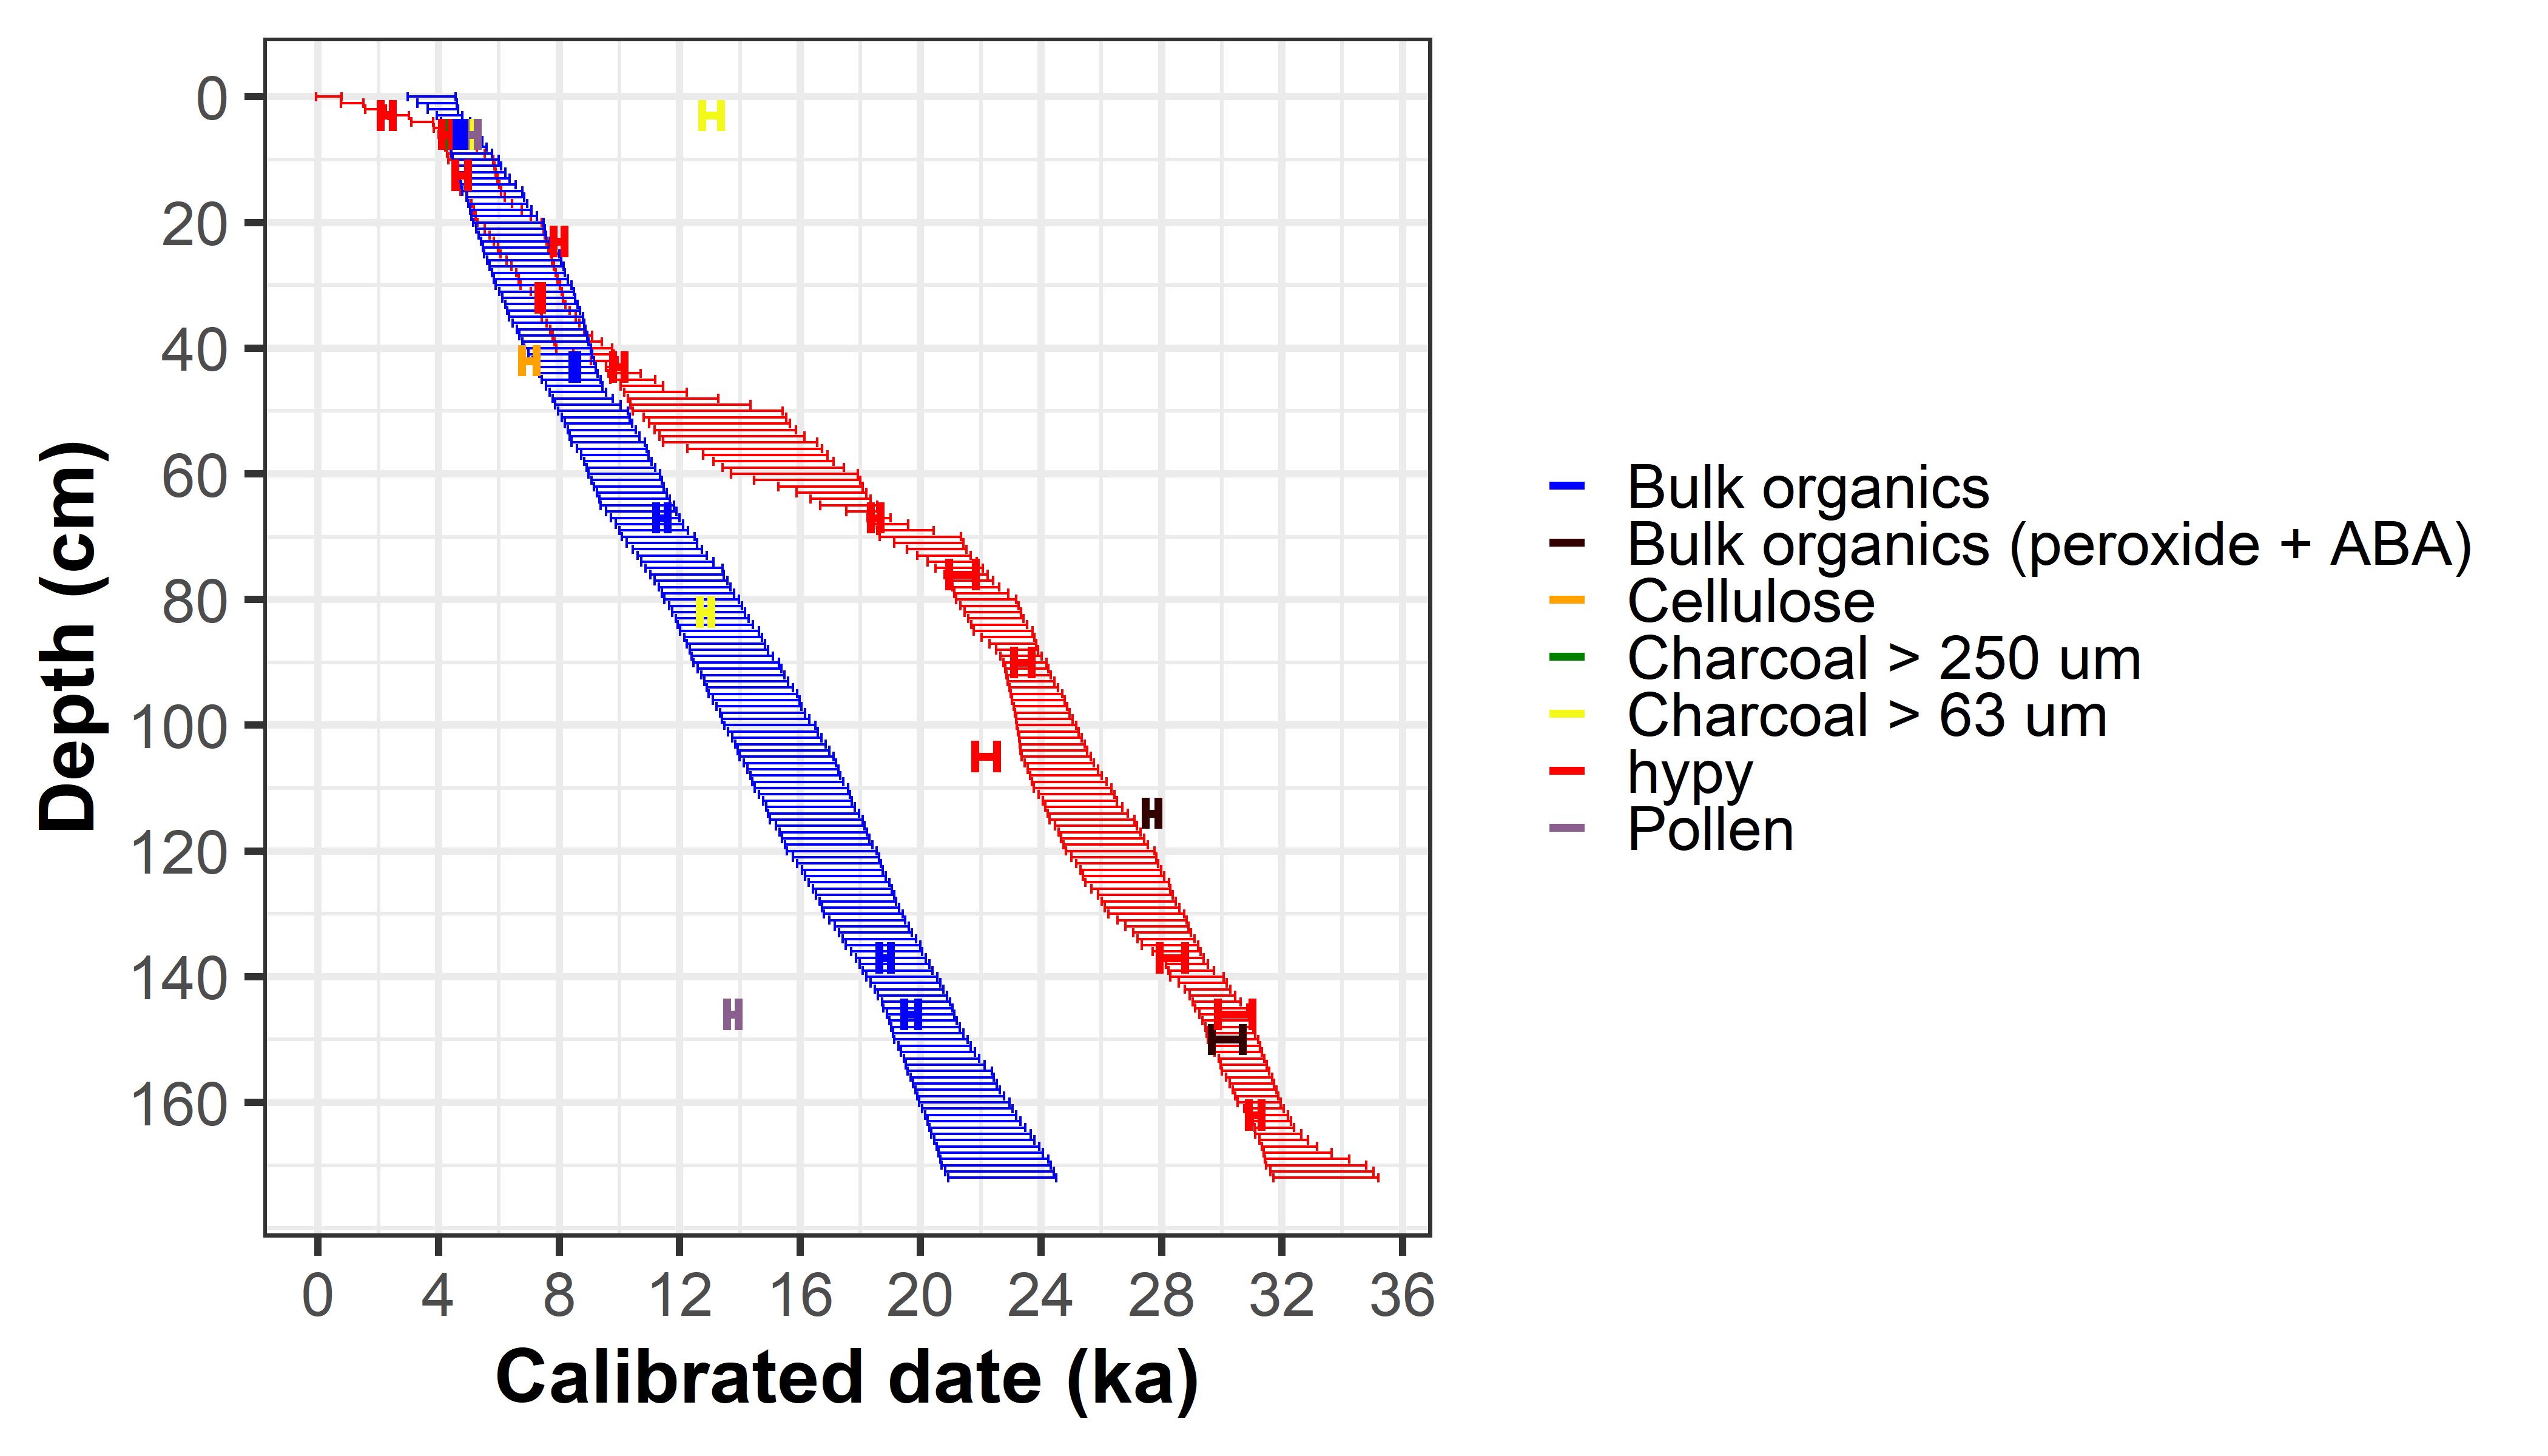
\includegraphics[width=0.8\linewidth]{C:/Users/Maria Jose Rivera/Documents/PhD/Figs/models_RC_2} 

}

\caption{Age-depth models (95 \% confidence error bars) constructed using Bayesian age modelling with rbacon package in R. Chronology based on Hypy is represented in turquoise and chronology based on bulk organics in blue, along with the calibrated dates from additional carbon fractions, none used in the construction of either chronology.}\label{fig:modelsb}
\end{figure}



Finally, the results from this study highlight the importance of comparing the results from different fractions (when using radiocarbon dating) or contrasting the dates from multiple dating methods when building to support the construction of palaeoenvironmental proxy records and comparing results those derived from other dating methods. Caution should be exercised when interpreting chronologies derived from bulk organics carbon fractions. Although the chronology obtained using bulk organics with the standard ABA-pretreatment method appeared to be consistent and with no age reversals, hypy provides the most robust chronology for the Sanamere Lagoon sequence and indicate the bulk organics chronology to be incorrect.

\hypertarget{chapter-summary}{%
\section{Chapter summary}\label{chapter-summary}}

The selection and pre-treatment of a reliable organic fraction from which to acquire radiocarbon dates is fundamental to the development of accurate and precise chronologies. Sampling from tropical lakes is particularly challenging given the adverse preservation conditions and diagenesis in these environments. This chapter examines and quantifies the differences between the radiocarbon date results and reliability from different carbon fractions and pretreatments from the same depths from Sanamere Lagoon, a tropical lake sediment core (1.72 m long)

located in north Australia. Six different organic fractions (bulk organics, pollen concentrate, cellulose, stable polycyclic aromatic carbon (SPAC), charcoal \textgreater250 um and charcoal \textgreater63 um), for a total of 27 radiocarbon dates, were compared in six different depths along the core. Acid-base-acid (ABA), modified ABA (30 \% hydrogen peroxide + ABA), 2chlorOx (a novel cellulose pre-treatment method) and hydrogen pyrolysis (hypy) were used to pre-treat the correspondent organic fractions.
The oldest date is 31.3 ka and the youngest is 2.5 ka, spanning 29,247 years. The smallest offset between the minimum and the maximum age in a given depth was found to be 975 years (between SPAC and charcoal \textgreater63 um) and the largest 16,527 years (between pollen concentrate and SPAC). The SPAC fractions pre-treated with hypy yielded older ages compared to all other fraction in most cases, while bulk organics consistently yielded younger ages. The magnitude and consistency of the offsets and the physical and chemical properties of the tested organic fractions suggest that SPAC is the most reliable fraction to date in tropical lake sediments and that hypy successfully removes contamination sourced from exogenous carbon.
The Sanamere Lagoon chronology was built exclusively using samples pretreated with hypy. Hypy outperforms the other procedures to pretreat samples for radiocarbon dating, and it was the most consistent with the stratigraphical changes found in the core.







  \bibliography{final\_ref\_2.bib}

\end{document}
